%This template was prepared by Dorothea F. Brosius of the 
%Institute for Electronics and Applied Physics, University of Maryland, College Park, MD
%The template was last updated in March 2013
%Thesis Main Page used with thesis.sty based on the
%University of Maryland Electronic Thesis and Dissertation (ETD) Style Guide

\documentclass[12pt]{report}

% Control chapter headings -- this is REQUIRED for compliance with UMD style requirements.
\usepackage{titlesec}
\titleformat{\chapter}[block]{\LARGE\bfseries}{\chaptertitlename\ \thechapter:}{20pt}{}
\titlespacing*{\chapter}{0pt}{0.5in}{1in}

\usepackage{hyperref} % Create hyperlinks.
\usepackage{cite} % When multiple citations are listed together, automatically convert to a reference range.
\usepackage{color} % Enable colors (useful to make sure I notice things I want to return to).
\usepackage{amsmath} % For producing high-quality multi-line math displays.
\usepackage{IEEEtrantools} % Alternative for complicated math -- allows specifying column alignment.
\usepackage{verbatim} % For producing blocks of comments.
\usepackage{setspace} % Permit us to single-space sections like tables, as permitted by UMD guidelines.
\usepackage{algorithmic} % For producing algorithms.
\usepackage{algorithm} % For producing floating figures which hold an algorithmic environment.
\usepackage{multirow} % For merging table entries vertically.
\usepackage{graphicx} % To include graphics.
\usepackage{notoccite} % Prevent citations in figure captions from affecting numbering.

\newcommand{\tbsp}{\rule{0pt}{18pt}} %used to get a vertical distance after \hline
\renewcommand{\baselinestretch}{2}
\setlength{\textwidth}{5.9in}
\setlength{\textheight}{9in}
\setlength{\topmargin}{-.50in}
%\setlength{\topmargin}{0in}    %use this setting if the printer makes the the top margin 1/2 inch instead of 1 inch
\setlength{\oddsidemargin}{.55in}
\setlength{\parindent}{.4in}
\pagestyle{empty}

\begin{document}

%Abstract Page 

\hbox{\ }

\renewcommand{\baselinestretch}{1}
\small \normalsize

\begin{center}
\large{{ABSTRACT}} 

\vspace{3em} 

\end{center}
\hspace{-.15in}
\begin{tabular}{ll}
Title of dissertation:    & {\large A Search for the Neutrinoless Double Beta Decay}\\
&                           {\large of Xenon-136 with Improved} \\
&                           {\large Sensitivity from Waveform Denoising} \\
\ \\
&                          {\large  Clayton G. Davis, Doctor of Philosophy, 2014} \\
\ \\
Dissertation directed by: & {\large  Professor Carter Hall} \\
&  				{\large	 Department of Physics } \\
\end{tabular}

\vspace{3em}

\renewcommand{\baselinestretch}{2}
\large \normalsize

\singlespace{
The EXO-200 detector is designed to search for a theorized decay process of xenon-136 called neutrinoless double-beta ($\beta\beta 0\nu$) decay.  $\beta\beta 0\nu$ decay, if it occurs, would have important consequences for our understanding of the neutrino sector of the standard model.  It would demonstrate the type of the neutrino mass term; set the mass scale of the neutrino sector; and demonstrate the first direct observation of lepton number non-conservation.  The $\beta\beta 0\nu$ decay produces a monoenergetic peak, so one important approach to reducing backgrounds for this search is by improving the energy resolution of the detector.

The present work describes a new analysis technique which improves resolution in the scintillation channel by a combination of waveform denoising and weighting of waveform components based on their expected signal-to-noise ratio; the overall resolution of the detector is improved by better than $20\%$.  Application of this method results in a halflife limit on $\beta\beta 0\nu$ decay in xenon-136 of $T_{1/2} > 1.1 \cdot 10^{25}$ years at $90\%$ confidence.  Further improvements which could impact the energy resolution of EXO-200 are also described, and implications for the planned nEXO experiment are considered.
}
 %(must be first, required, non-numbered)
%Titlepage

\thispagestyle{empty}
\hbox{\ }
\vspace{1in}
\renewcommand{\baselinestretch}{1}
\small\normalsize
\begin{center}

\large{{SIGNAL DENOISING FOR EXO-200 AND AN IMPROVED LIMIT ON NEUTRINOLESS DOUBLE-BETA DECAY}}\\
\ \\
\ \\
\large{by} \\
\ \\
\large{Clayton G. Davis}%Your full name as it appears in University records.
\ \\
\ \\
\ \\
\ \\
\normalsize
Dissertation submitted to the Faculty of the Graduate School of the \\
University of Maryland, College Park in partial fulfillment \\
of the requirements for the degree of \\
Doctor of Philosophy \\
2014
\end{center}

\vspace{7.5em}

\noindent Advisory Committee: \\
Professor Carter Hall, Chair/Advisor \\
Professor Radu Balan \\
Professor Betsy Beise \\
Professor Rabindra Mohapatra \\
Professor Peter Shawhan
 %(must follow Abstract, required, non-numbered)
%Copyright

\thispagestyle{empty}
\hbox{\ }

\vfill
\renewcommand{\baselinestretch}{1}
\small\normalsize

\vspace{-.65in}

\begin{center}
\large{\copyright \hbox{ }Copyright by\\
Clayton Davis  %Type your name as it appears in University records
\\
2014}
\end{center}

\vfill
 %(highly recommended, non-numbered)

%Pages from this point start at lower-case Roman number ii)
\pagestyle{plain}
\pagenumbering{roman}
\setcounter{page}{2}

%Dedication

\renewcommand{\baselinestretch}{2}
\small\normalsize
\hbox{\ }
 
\vspace{-.65in}

\begin{center}
\large{Dedication}
\end{center} 

If needed.
 %(if present, lower-case Roman)
%Acknowledgments

\renewcommand{\baselinestretch}{2}
\small\normalsize
\hbox{\ }
 
\vspace{-.65in}

\begin{center}
\large{Acknowledgments} 
\end{center} 

\vspace{1ex}

Without the help of my colleagues, advisor, friends, family, and my wife, this thesis and the work it embodies would never have happened.  I would like to give thanks to the EXO-200 collaboration, which has provided a supportive and stimulating environment for my work and learning over the past four years.

Particular thanks must go to: David Auty, Phil Barbeau, Giorgio Gratta, Steve Herrin, Sam Homiller, Mike Jewell, Tessa Johnson, Tony Johnson, Caio Licciardi, Mike Marino, Dave Moore, Russell Neilson, Igor Ostrovskiy, J.J. Russell, Kevin O'Sullivan, Tony Waite, Josiah Walton, Liangjian Wen, Liang Yang, and of course my advisor Carter Hall.  I can honestly say that each one of you directly made the following work possible with your contribution of insight, data, plots, and analysis.  Denoising has been a tremendously collaborative effort, and I am grateful that my last project with this group has provided the chance to work with all of you so closely.
 %(if present, lower-case Roman)

\renewcommand{\baselinestretch}{1}
\small\normalsize
\tableofcontents %(required, lower-case Roman)
\newpage
%\listoftables %(if present, lower-case Roman)
%\newpage
\phantomsection % Needed to make hyperlinks point to the right page.
\addcontentsline{toc}{chapter}{List of Figures} % Adds section to table of contents.
\listoffigures %(if present, lower-case Roman)
\newpage
% LIST OF ABBREVIATIONS
\phantomsection % Needed to make hyperlinks point to the right page.
\addcontentsline{toc}{chapter}{List of Abbreviations} % Adds section to table of contents.
%List of Abbreviations

\renewcommand{\baselinestretch}{1}
\small\normalsize
\hbox{\ }

\vspace{-4em}

\begin{center}
\large{List of Abbreviations}
\end{center} 

\vspace{3pt}

\begin{tabular}{ll}
EXO & Enriched Xenon Observatory \\
APD & Avalanche Photo-diode \\
\end{tabular}


\newpage
\setlength{\parskip}{0em}
\renewcommand{\baselinestretch}{2}
\small\normalsize

%Pages from this point start at Arabic numeral 1
\setcounter{page}{1}
\pagenumbering{arabic}
\renewcommand{\thechapter}{1}
\chapter{Introduction}
\label{ch:Introduction}

The EXO-200 detector is designed to search for a theorized decay mode of xenon-136 by emission of two electrons and no neutrinos.  Neutrinoless double-beta ($\beta\beta 0\nu$) decay, if it occurs, would have far-reaching implications: it would set the absolute mass scale of the neutrino sector, provide clues to the mechanism which generates mass in the neutrino sector, and give the first direct observation of non-conservation of lepton number.

EXO-200 contains roughly 110 kg of liquid xenon in its active volume.  The xenon used by EXO has been enriched to $80.6\%$ in xenon-136, resulting in approximately $3.9 \times 10^{26}$ atoms of $^{136}$Xe which can be observed in the EXO-200 detector.  The observation of $\beta\beta 0\nu$ decay would present itself as a peak in the energy spectrum at a Q-value of $2458$ keV, so EXO-200 is designed to produce a peak at this energy which is subject to as little background as possible.

Background is controlled primarily by reducing the level of radioactivity of materials in and around the liquid xenon.  All materials used in the construction of the EXO-200 detector were carefully screened for low concentration of radioactive backgrounds, making the EXO-200 detector one of the lowest-background detectors in the world.

After construction, background reduction must be performed by discrimination between $\beta\beta 0\nu$ and other processes.  This can be performed primarily by exploiting the event topology and by refining the energy measurements.  The event topology of $\beta\beta 0\nu$ consists of a highly localized energy deposit due to the short interaction length of $\beta$ particles; by contrast, backgrounds will often produce diffuse energy deposits which can be rejected as candidate $\beta\beta 0\nu$ events.

Perhaps the most straightforward method of background reduction, however, is by energy.  An improved energy resolution assures us that $\beta\beta 0\nu$ candidate events must come from a narrower region of the energy spectrum and lets us reject events outside of that region of interest (ROI).  The EXO-200 detector observes energy in two forms, ionization (charge) and scintillation (light), and both are necessary to achieve excellent energy resolution.  The scintillation measurement has a lower accuracy, so it is the limiting factor to the energy resolution of EXO-200.

In this work, we describe a new technique for improving the accuracy of the scintillation measurements of the EXO-200 detector through a detailed offline waveform analysis.  This technique, identified throughout this work as ``denoising'', consists of understanding the signal-to-noise ratio of the different components of our scintillation measurement.  The signal-to-noise content of our scintillation measurements depends on both the proximity of a light sensor to the energy deposit and on the spectral shape of light pulses compared to waveform noise.  An active noise reduction program is included in this effort, which in turn improves the signal-to-noise content of the scintillation measurements.  An overall improvement in the EXO-200 energy resolution of more that $20\%$ is achieved at the Q-value.

We provide an overview of the theoretical motivations for the search for $\beta\beta 0\nu$ decay in chapter~\ref{ch:BB0NTheory}.  Chapter~\ref{ch:EXO200Detector} describes the design of the EXO-200 detector, the backgrounds it expects, and some of the techniques it is capable of using to reduce those backgrounds.  Chapter~\ref{ch:DenoisingTheory} derives the mathematical framework of denoising and some practical considerations of its application; chapters~\ref{ch:NoiseMeasurements} and \ref{ch:Lightmap} describe the measurements of electronic noise and light yield which are critical inputs to denoising.  In chapter~\ref{ch:DenoisingResults} we describe the components and results of the EXO-200 analysis, including comparisons between results with and without denoising in sections~\ref{sec:RotatedEnergyCalibration} and \ref{sec:ResultComparison}.  Conclusions and future outlook are contained in chapter~\ref{ch:Conclusions}.

\renewcommand{\thechapter}{2}
\chapter{Theory of Neutrinoless Double-Beta Decay}
\label{ch:BB0NTheory}

Toward the end of the 1990s neutrinos were conclusively proven to possess a non-zero mass.  Subsequent effort has been directed toward understanding the absolute scale of neutrino mass spectrum and the nature of the interaction which causes it.  Neutrinoless double-beta ($\beta\beta 0\nu$) decay, would provide a window onto both questions.  This chapter presents the theoretical motivations for searching for $\beta\beta 0\nu$ decay.  Section~\ref{sec:TheoryStandardDoubleBeta} describes the closely-related two-neutrino double-beta ($\beta\beta 2\nu$) decay which is allowed in the standard model.  Section~\ref{sec:TheoryNeutrinolessDoubleBeta} defines $\beta\beta 0\nu$ decay and reasons for hypothesizing its occurrence.  Considerations and challenges in nuclear physics are described in section~\ref{sec:NuclearMatrixCalculations}.  The parametrization of the neutrino sector is provided in section~\ref{sec:NeutrinoFlavorPhysics}.  Section \ref{sec:ParticlePhysicsConstraints} summarizes constraints on neutrino masses which can be obtained from observations of single-$\beta$ decay and cosmology, and section \ref{sec:NucPhysConstraintsFromBB0N} describes in detail the considerations and challenges involved in searching for $\beta\beta 0\nu$ decay.  The reader will obtain a general understanding of the state of the field before continuing on to the details of the EXO-200 detector in chapter~\ref{ch:EXO200Detector}.

\begin{figure}
\begin{center}
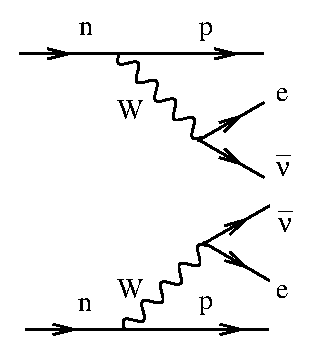
\includegraphics[keepaspectratio=true,width=2in]{Avignone_fig02a.eps}
\end{center}
\renewcommand{\baselinestretch}{1}
\small\normalsize
\begin{quote}
\caption{Feynman diagram for $\beta\beta 2 \nu$ decay.  The reaction products are equivalent to two $\beta$ decays in succession, but this reaction can sometimes occur even if a single $\beta$ decay would be energetically forbidden.  Figure from~\cite{RMPbb0n}.}
\label{fig:FeynmanBetaBeta2Nu}
\end{quote}
\end{figure}
\renewcommand{\baselinestretch}{2}
\small\normalsize

\section{Two-Neutrino Double-Beta Decay}\label{sec:TheoryStandardDoubleBeta}

Standard-model two-neutrino double beta ($\beta\beta 2\nu$) decay is the result of the particle interaction
\begin{equation}\label{eqn:bb2n_decay_reaction}
2d \rightarrow 2u + 2e^- + 2\bar{\nu}_e
\end{equation}
mediated by $W^-$-exchange, as depicted in Figure~\ref{fig:FeynmanBetaBeta2Nu}.  It is effectively the simultaneous occurrence of two beta ($\beta$) decays from the same nucleus.

Because $\beta\beta 2\nu$ decay is a second-order weak interaction, it has a remarkably slow rate compared to most $\beta$ decay processes.  Although many nuclei are expected to decay by $\beta\beta 2\nu$, the process is thoroughly masked by conventional $\beta$ decay in most of them.  In most cases, we can only hope to detect $\beta\beta 2\nu$ decay in isotopes where $\beta$ decay is forbidden or highly suppressed.

An example of an isotope for which $\beta$ decay is highly suppressed is $^{48}_{20}$Ca.  The ground state of $^{48}_{20}$Ca has zero units of angular momentum, whereas its single-$\beta$ decay daughter product $^{48}_{21}$Sc has six units of total angular momentum in its ground state, and is thus highly suppressed by angular momentum conservation.  In contrast, $^{48}_{22}$Ti has zero units of total angular momentum, making $\beta\beta 2\nu$ decay of $^{48}_{20}$Ca permitted by angular momentum and energy considerations, and as a result the $\beta\beta 2\nu$ decay mode of $^{48}_{20}$Ca dominates~\cite{MyNuclearPhysicsBook}.

In the most promising $\beta\beta 2\nu$ candidates, single $\beta$ decay is forbidden by energy conservation.  It is well-known that nuclei minimize their energy by arranging similar nucleons to have overlapping wavefunctions~\cite{MyNuclearPhysicsBook}.  Thus, isotopes with an even number of protons and an even number of neutrons will have less nucleon-pairing potential energy than an isotope with either an odd number of protons or an odd number of neutrons, which in turn will have less nucleon-pairing potential energy than an isotope with an odd number of protons and an odd number of neutrons.

\begin{figure}
\begin{center}
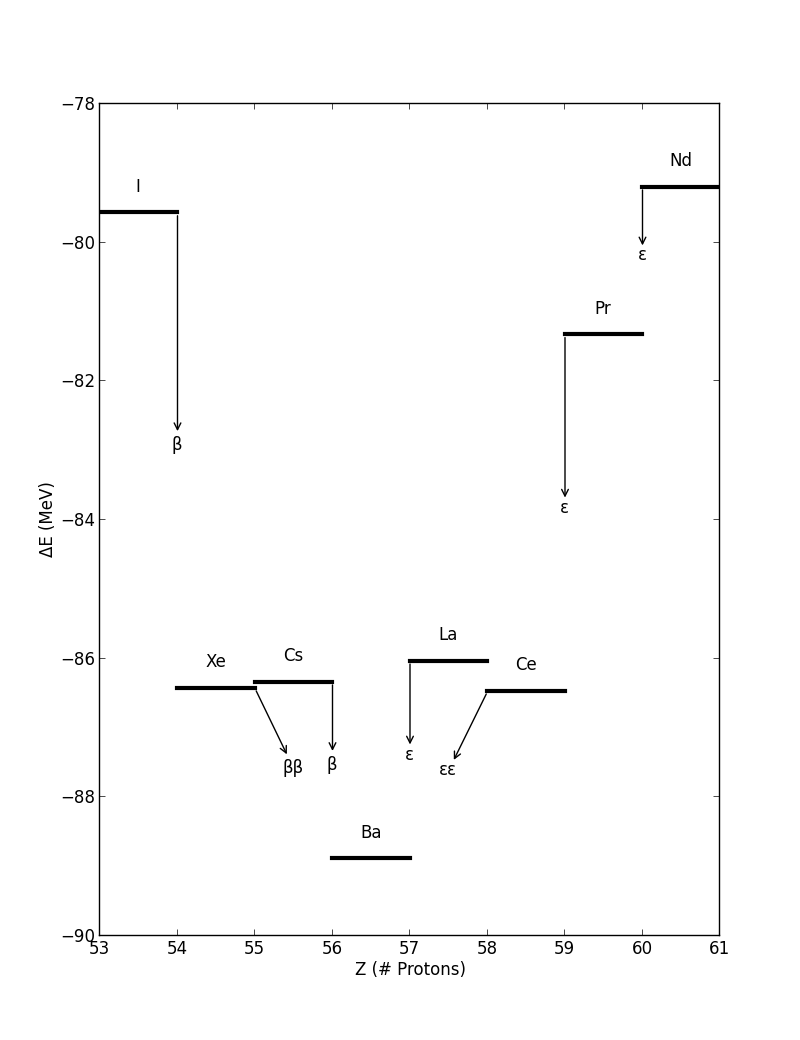
\includegraphics[keepaspectratio=true,width=\textwidth]{scripts/LevelDiagram.png}
\end{center}
\renewcommand{\baselinestretch}{1}
\small\normalsize
\begin{quote}
\caption{Energy diagram of isotopes with atomic mass $A=136$.  The energies $\Delta E$ are the binding energies of the atom, compared to the bare masses of the same nuclei.  Values are from~\cite{AtomicMassEvaluation}.}
\label{fig:LevelDiagram}
\end{quote}
\end{figure}
\renewcommand{\baselinestretch}{2}
\small\normalsize

The effect is illustrated by the nuclear energy level diagram shown in figure~\ref{fig:LevelDiagram} for the $A=136$ isobar. Xenon, barium, cerium, and neodymium are even-even isotopes, and have systematically lower energies than the odd-odd isotopes iodine, cesium, lanthanum, and praseodymium.  For this particular isobar, we can see that xenon is energetically forbidden from single-$\beta$ decaying to cesium because the odd-odd isotope of cesium has slightly more potential energy than the even-even isotope of xenon. As a result, the primary mode of decay of xenon-136 will be $\beta\beta 2\nu$ decay to barium-136.  Similarly, cerium-136 can undergo double-electron capture, electron capture with positron emission, or double-positron emission; however, in practice the expected rates for these decays will be lower than the rates for $\beta\beta 2\nu$ decay, so we will not consider them further in this work.

\section{Neutrinoless Double-Beta Decay}\label{sec:TheoryNeutrinolessDoubleBeta}

The detection and study of $\beta\beta 2\nu$ decay provides an opportunity to test a class of nuclear matrix element computations; however, the decay does not violate any fundamental symmetries and its existence is, in this sense, a mundane prediction of the Standard Model.  The primary appeal of isotopes which undergo $\beta\beta 2\nu$ decay is the opportunity these isotopes provide to probe the nature of neutrinos through the related neutrinoless decay.

It had been suggested as early as 1937 that neutrinos could possess mass through a neutrino-antineutrino interaction, provided that the neutrino is its own antiparticle~\cite{Majorana}.  The theorized Majorana interaction comes from Lagrangian terms of the form (for each of three neutrino eigenstates)
\begin{align}
\mathcal{L}_{Maj}&= \begin{aligned}[t]
 & -\frac{m_{L}}{2} \left( \overline{\Psi_L^c} \Psi_L^{} + \overline{\Psi_L^{}} \Psi_L^c \right)\\
 & -\frac{m_{R}}{2} \left( \overline{\Psi_R^c} \Psi_R^{} + \overline{\Psi_R^{}} \Psi_R^c \right),
\end{aligned}\label{eqn:MajoranaLagrangianTerms}
\end{align}
where the superscript-$c$ represents charge conjugation.  (This is the reason that Majorana mass terms are only possible for a chargeless lepton.)  The masses $m_L$ and $m_R$ may be chosen independently; since there has never been an observation of right-handed neutrinos or left-handed anti-neutrinos, it is possible that $m_R = 0$ and that the fields $\Psi_R^{}$ and $\Psi_R^c$ do not exist in nature~\cite{RMPbb0n}.

\begin{figure}
\begin{center}
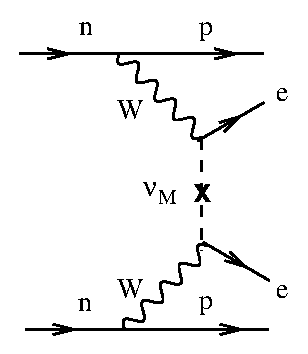
\includegraphics[keepaspectratio=true,width=2in]{Avignone_fig02b.eps}
\end{center}
\renewcommand{\baselinestretch}{1}
\small\normalsize
\begin{quote}
\caption{Feynman diagram for $\beta\beta 0 \nu$ decay.  A virtual neutrino mediates the exchange.  This is only possible if $\overline{\nu}_R$ can flip its handedness to $\nu_L$, and the interaction that induces this parity change also generates neutrino mass.  Figure from~\cite{RMPbb0n}.}
\label{fig:FeynmanBetaBeta0Nu}
\end{quote}
\end{figure}
\renewcommand{\baselinestretch}{2}
\small\normalsize

If neutrinos do have Majorana mass interactions, then any isotope that undergoes $\beta\beta 2\nu$ decay can also undergo the related process $2d \rightarrow 2u + 2e^-$, depicted in Figure~\ref{fig:FeynmanBetaBeta0Nu}, in which the two outgoing neutrinos in $\beta\beta 2\nu$ decay are replaced by one virtual neutrino.  This process is called neutrinoless double-beta ($\beta\beta 0\nu$) decay.  We can interpret this as a mixing interaction between a left-handed neutrino and a right-handed antineutrino; this is only possible if neutrinos are Majorana particles.

The tree-level diagram for $\beta\beta 0\nu$ has one additional interaction vertex compared to $\beta\beta 2\nu$ decay, and as a result we would expect it to occur at an even slower rate.  However, the more immediate consequence of $\beta\beta 0\nu$ decay is that lepton number conservation is violated.  The lepton number changes by two units corresponding to the creation of two leptons with no balancing anti-leptons.  Numerous theories have suggested other plausible modes of lepton number non-conservation~\cite{ProtonDecay,MuonToPositron}, but none have yet reported a positive result.  In the conventional Standard Model with massless neutrinos, lepton number conservation is an accidental symmetry~\cite{LeptonConservation}, but in a model with massive neutrinos there may no longer be any reason \textit{a priori} to expect conservation of lepton number.

\begin{figure}
\begin{center}
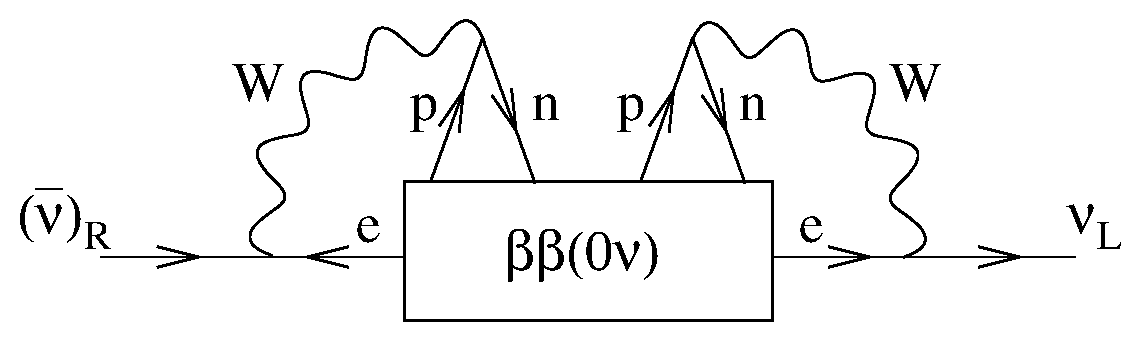
\includegraphics[keepaspectratio=true,width=\textwidth]{Avignone_fig03.eps}
\end{center}
\renewcommand{\baselinestretch}{1}
\small\normalsize
\begin{quote}
\caption{Even without any assumptions about the mechanism which leads to $\beta\beta 0\nu$ decay, we can use that process to generate an effective neutrino mass as a higher-order process.  Figure from~\cite{RMPbb0n}.}
\label{fig:FeynmanBetaBeta0NuImplication}
\end{quote}
\end{figure}
\renewcommand{\baselinestretch}{2}
\small\normalsize

It is worth noting that the interaction term above assumes no mediating particles in the mass mechanism, whereas it is possible that $\beta\beta 0\nu$ could be mediated by some higher-order interaction terms.  However, if $\beta\beta 0\nu$ decay is observed, it leads very generally to a conclusion that neutrinos have an \emph{effective} Majorana mass interaction~\cite{BlackBoxTheorem}.  We can see this by embedding the $\beta\beta 0\nu$ process into a higher-order one, as shown in figure~\ref{fig:FeynmanBetaBeta0NuImplication}.  Regardless of the details of how $\beta\beta 0\nu$ occurs, its existence would necessarily generate an effective neutrino mass as a higher-order process.

We have described so far only the theorized Majorana interaction of equation~\ref{eqn:MajoranaLagrangianTerms}.  However, it is also possible that neutrinos could have a Dirac mass term analogous to the other fermions.  The full set of neutrino mass terms in the Lagrangian would then be:
\begin{align}
\mathcal{L}_{Maj+Dirac}&= \begin{aligned}[t]
 & -\frac{m_{L}}{2} \left( \overline{\Psi_L^c} \Psi_L^{} + \overline{\Psi_L^{}} \Psi_L^c \right)\\
 & -\frac{m_{R}}{2} \left( \overline{\Psi_R^c} \Psi_R^{} + \overline{\Psi_R^{}} \Psi_R^c \right)\\
 & -m_D \left(\overline{\Psi_L}\Psi_R + \overline{\Psi_R}\Psi_L\right),
\end{aligned}
\end{align}
where $m_D$ is the new Dirac mass term.  The three flavors observed in nature would result in three sets of these terms, one for each flavor, and nine possible mass terms in total~\cite{RMPbb0n}.

For simplicity, we consider now the mass terms for a one-flavor system.   We can rearrange the Lagrangian terms as:
\begin{subequations}\begin{align}
\mathcal{L}_{Maj+Dirac}&= -\frac{1}{2} \left(\overline{\left(n_L\right)^c} \mathcal{M} n_L + \overline{\left(n_L\right)^{}} \mathcal{M} n_L^c\right), \text{where}\\
\mathcal{M}&= \begin{pmatrix}m_L & m_D \\ m_D & m_R \end{pmatrix}\\
n_L &= \begin{pmatrix} \Psi_L \\ \left(\Psi_R\right)^c \end{pmatrix}.
\end{align}\end{subequations}
The matrix $\mathcal{M}$ can, in all cases, be diagonalized by some unitary matrix, which means that there is always a basis in which two interaction terms are sufficient.  In nearly all cases the eigenvalues will be distinct values, so the two eigenstates are non-degenerate.  Both eigenstates in this case are their own antiparticles, so they are Majorana.  The only exceptions to this are when $m_L = m_R$ and $m_D = 0$, or when $m_L = m_R = 0$.  Both of those special cases lead to degenerate eigenspaces; in the former, the system is clearly purely Majorana from the beginning, and in the latter the system is purely Dirac.  Thus we can see that even though it is possible to include a Dirac neutrino mass term, neutrinos will be Majorana particles unless $m_L = m_R = 0$.  Similar results hold in the three-flavor case~\cite{RMPbb0n}.

We have spoken of the possibility that the Majorana mass term comes from a tree-level Lagrangian term.  However, this would be a surprising result.  The Majorana fields would not have the same quantum number under the $SU(2)_L\times SU(2)_R$ symmetry, meaning that either neutrinos would need to choose between the Majorana and Dirac terms or some larger symmetry would need to take the place of $SU(2)_L\times SU(2)_R$.  It is viewed as more likely that neutrino mass is generated through an effective interaction.  A natural mechanism to generate neutrino mass called the see-saw mechanism was developed around 1980~\cite{PhysRevLett.44.912,GellMann:1980vs}.  In this scheme we presume that $m_R \gg m_D \gg m_L$.  The Dirac term could come from the Higgs mechanism, so we expect $m_D$ to occupy the 1 MeV energy range typical of other leptons and quarks.  The large mass $m_R$ of the right-handed neutrino $\nu_R$ is meant to explain the absence of $\nu_R$ and $\overline{\nu_R^c}$ from all observations.  When we take $m_L = 0$ and diagonalize the single-flavor neutrino mass matrix $\mathcal{M}$ we obtain:
\begin{align}
\mathcal{M} &= \begin{pmatrix}0 & m_D \\ m_D & m_R \end{pmatrix}\\
&\propto \begin{pmatrix} \mathrm{i} & m_D/m_R \\ -\mathrm{i}m_D/m_R & 1 \end{pmatrix}
\begin{pmatrix} -m_D^2/m_R & 0 \\ 0 & m_R\end{pmatrix}
\begin{pmatrix}-\mathrm{i} & \mathrm{i}m_D/m_R \\ m_D/m_R & 1 \end{pmatrix}.
\end{align}
In other words, if we presume that there is a Dirac neutrino mass similar to the masses of other leptons and a right-handed Majorana neutrino mass $m_R \gg m_D$, then in another basis a small left-handed Majorana neutrino mass $m_D^2/m_R$ is generated.  This is widely considered to be the most natural mechanism for explaining the lightness of the neutrinos observed in nature~\cite{RMPbb0n,mohapatra1998massive}.

\begin{figure}
\begin{center}
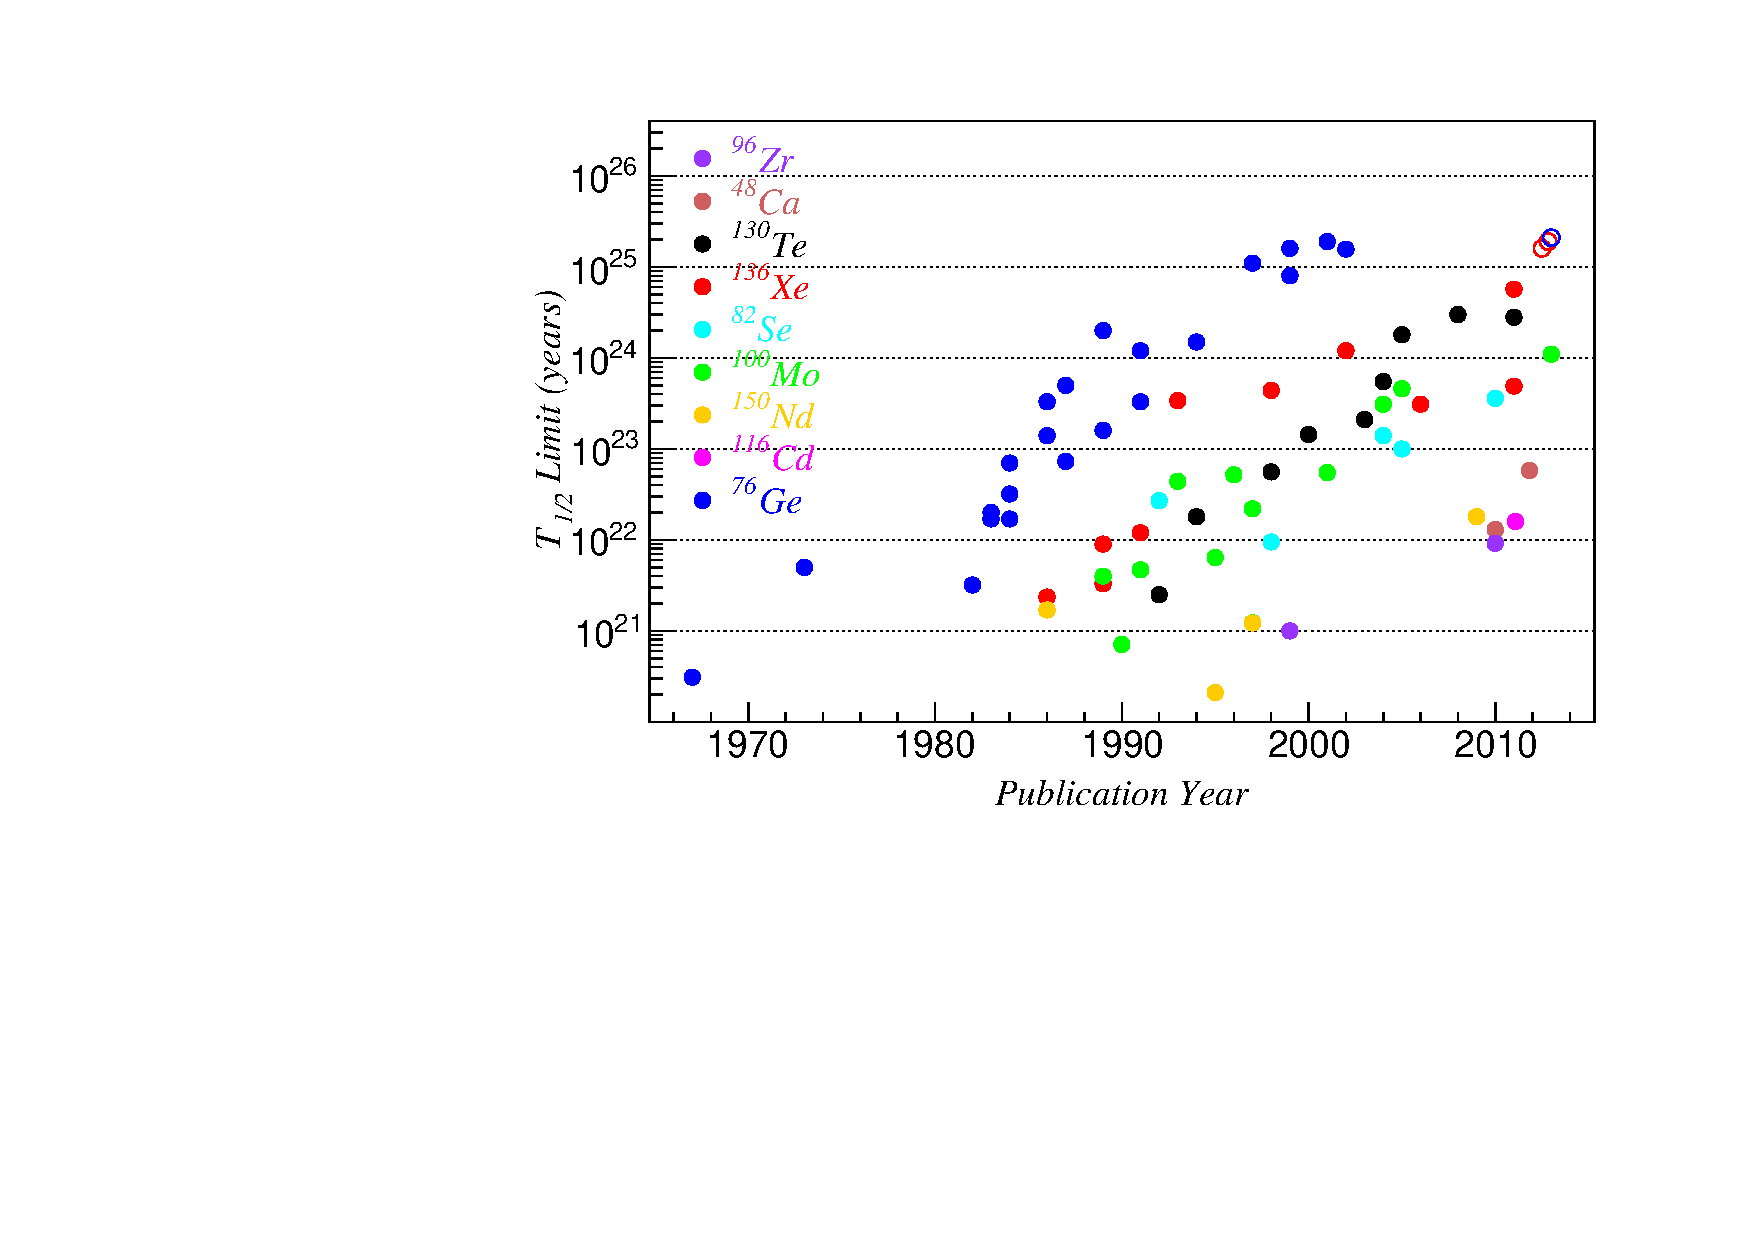
\includegraphics[keepaspectratio=true,width=\textwidth]{halflife_vs_year.pdf}
\end{center}
\renewcommand{\baselinestretch}{1}
\small\normalsize
\begin{quote}
\caption{A selection of $\beta\beta 0\nu$ half-life limits versus the publication year of the limit.  Colors indicate which isotope is under study.  Open circles indicate experiments which have not yet concluded data-taking.  Data is from ~\cite{
PhysRevC.85.045504,PhysRevLett.110.062502,bb0nSearch2012,PhysRevLett.111.122503,
KlapdorDissent,PhysRevLett.83.41,PhysRevC.59.2108,PhysRevD.65.092007,Andreotti2011822,PhysRevC.78.035502,
PhysRevLett.95.142501,Arnaboldi2004260,Baudis1997219,PhysRevLett.95.182302,NEMO2004,NEMO3-2013-100Mo,
doi:10.1142/S0217732390001475,Bernabei200223,Balysh1994176,0954-3899-17-S-014,Arnaboldi2003167,
1112.0859,Baksan2006Gavriljuk,Luescher1998407,Alessandrello1992176,Alessandrello1994519,Alessandrello1998156,
Alessandrello200013,PhysRevD.48.1009,PhysRevLett.59.419,Bellotti1991193,Bellotti1989209,BellottiMilano1986,
Bellotti1984450,Bellotti198372,BellottiMilano1982,PhysRevD.45.2548,PhysRevC.63.065501,0305-4616-13-6-012,
Ejiri199685,Ejiri199117,PhysRevC.55.474,PhysRevLett.71.831,PhysRevLett.63.1671,Fisher1989257,
PhysRevLett.50.721,PhysRevC.34.666,PhysRevLett.53.141,PhysRevD.51.2090,Forster1984301,PhysRevC.56.2451,
Barabash1989273,Fiorini1967602,Fiorini1973,Barabanov:1986iz,Vasilev:1990gi,PhysRevC.38.895}.}
\label{fig:Halflife_vs_year}
\end{quote}
\end{figure}
\renewcommand{\baselinestretch}{2}
\small\normalsize

A selection of $\beta\beta 0\nu$ half-life limits are shown in figure~\ref{fig:Halflife_vs_year} for the $^{76}$Ge, $^{100}$Mo, $^{130}$Te, and $^{136}$Xe isotopes with the publication year of the result.  Although some results did exist before 1980, after the publication of the see-saw mechanism in~\cite{PhysRevLett.44.912,GellMann:1980vs} experimental interest in neutrinoless double-beta decay flourished, and we can see that for the last thirty years there has been steady progress in improving experimental sensitivity for many isotopes.  The discovery by \cite{SuperK} in 1998 of oscillation of atmospheric neutrinos verified that neutrinos do have finite mass of some sort, adding to the motivation to search for the $\beta\beta 0\nu$ process.  The following sections describe computational and experimental considerations associated with searches for $\beta\beta 0\nu$ decay.

\section{Double-beta Decay Nuclear Matrix Calculations}\label{sec:NuclearMatrixCalculations}

If the dominant mechanism of $\beta\beta 0\nu$ decay is a tree level neutrino mass term as shown in figure~\ref{fig:FeynmanBetaBeta0Nu}, then the rate of $\beta\beta 0\nu$ decay will also reflect the magnitude of the neutrino mass parameters.  To specify this relation precisely we need an understanding of the nuclear physics of the decaying isotope.  This section will identify the relevant quantities which must be computed and provide a survey of the computational approaches to estimating them.

For a tree-level Majorana interaction we can write the partial half-life $T^{0\nu}_{1/2}$ of an isotope which undergoes $\beta\beta 0\nu$ decay as
\begin{equation}\label{eqn:HalfLifeMatrixElementEqn}
\left[T^{0\nu}_{1/2}\right]^{-1} = G_{0\nu}(Q_{\beta\beta}, Z) \left| M_{0\nu}\right|^2 \left< m_{\beta\beta} \right>^2,
\end{equation}
where $G_{0\nu}(Q_{\beta\beta}, Z)$ is a phase-space factor coming from the range of possible output states, $M_{0\nu}$ is a nuclear matrix element, and $\left< m_{\beta\beta} \right>$ is the effective $\beta\beta 0\nu$ neutrino mass which will be defined in section~\ref{sec:NucPhysConstraintsFromBB0N}.

The two factors $G_{0\nu}(Q_{\beta\beta}, Z)$ and $M_{0\nu}$ may be computed by a variety of methods, and it is tempting to draw nuclear matrix elements and phase factors from different publications.  However, this must be done carefully: scaling factors can be absorbed from one into the other, and if nuclear matrix elements and phase space factors are calculated using different conventions, the result of combining them will not be correct.

For example, in early calculations, the nuclear matrix element and phase-space factor were generally computed in units of $\mathrm{fm}^{-1}$ and $\mathrm{yrs}^{-1} \mathrm{fm}^2$, respectively.  Starting in the mid-1980s common practice shifted to multiply the nuclear matrix element by the nuclear radius $R_0 \propto A^3$, where $A$ is the number of nucleons, and divide the phase-space factor by $R_0^2$, making the nuclear matrix element unitless and the phase-space factor have units of $\mathrm{yrs}^{-1}$. With this convention care must be taken that the nuclear radius used in both calculations is the same, whereas for many years different authors might choose $R_0 = 1.1 A^3$ fm or $R_0 = 1.2 A^3$ fm without specifying that choice~\cite{PhysRevC.73.028501}.  Modern practice is now that the value of $R_0$ is explicitly specified in any matrix element or phase-space factor calculations. Another convention is whether the fourth power of the axial vector current $g_A^4$ should be included with the phase space factor, nuclear matrix element, or separately as its own factor of equation~\ref{eqn:HalfLifeMatrixElementEqn}, and again one must be careful to understand the chosen conventions before combining results from different sources~\cite{PhysRevC.87.014315}.

The phase-space factor $G_{0\nu}(Q_{\beta\beta}, Z)$ accounts for the phase space of the final state of $\beta\beta 0\nu$ decay.  This includes two outgoing electrons and the final state nucleus.  The mass of the outgoing nucleus is always much larger than the masses of the neutrinos, so nearly all momentum will be carried by the two electrons.  Each contributes a phase space integral of the form $\int_0^{p_{max}} \mathrm{d}\cdot p pE$, which individually contribute a factor proportional to $p_{max}^3$.  Considering the system in the rest frame of the initial state nucleus, the sum of the two electron momenta are constrained to be equal to zero, so the combined phase space integral for both electrons is proportional to
\begin{equation}
\int_0^{p_{max}} \mathrm{d}p_1 p_1E_1 \int_0^{p_{max}} \mathrm{d}p_2 p_2E_2 \delta(p_2-p_1) \propto p_{max}^5.
\end{equation}
As a result, the phase space factor $G_{0\nu}(Q_\beta\beta, Z)$ of $\beta\beta 0\nu$ decay will be proportional to $Q^5$, where $Q$ is the total energy of the decay~\cite{mohapatra1998massive}.  The strong dependence of $G_{0\nu}(Q_\beta\beta, Z)$ on $Q$ means that isotopes which have high $Q$-values will be expected to have shorter $\beta\beta 0\nu$ half-lives than isotopes with low $Q$-values, which is one reason that most $\beta\beta 0\nu$ searches focus on high-$Q$ isotopes.

Another important contribution to the phase space factor come from the electric potential of the atomic nucleus and its atomic electrons.  The potential $V(r)$ experienced by the escaping electron as a function radius is approximated by:~\cite{PhysRevC.87.014315}
\begin{equation}
V(r) = -Z \alpha \hbar c \cdot \begin{cases}
1/r & r \ge R_0 \\
\left(3-(r/R_0)^2\right)/2R_0 & r < R_0,
\end{cases}
\end{equation}
where $Z$ is the nuclear charge, $\alpha$ is the fine structure constant, $\hbar$ is Planck's constant, $c$ is the speed of light, and $R_0$ is the radius of the nucleus.  Higher-order corrections include the change in nuclear charge due to the decay and the density of the electron cloud (which includes angular asymmetries).  A modern treatment can be found in~\cite{PhysRevC.87.014315}.

\begin{figure}
\begin{center}
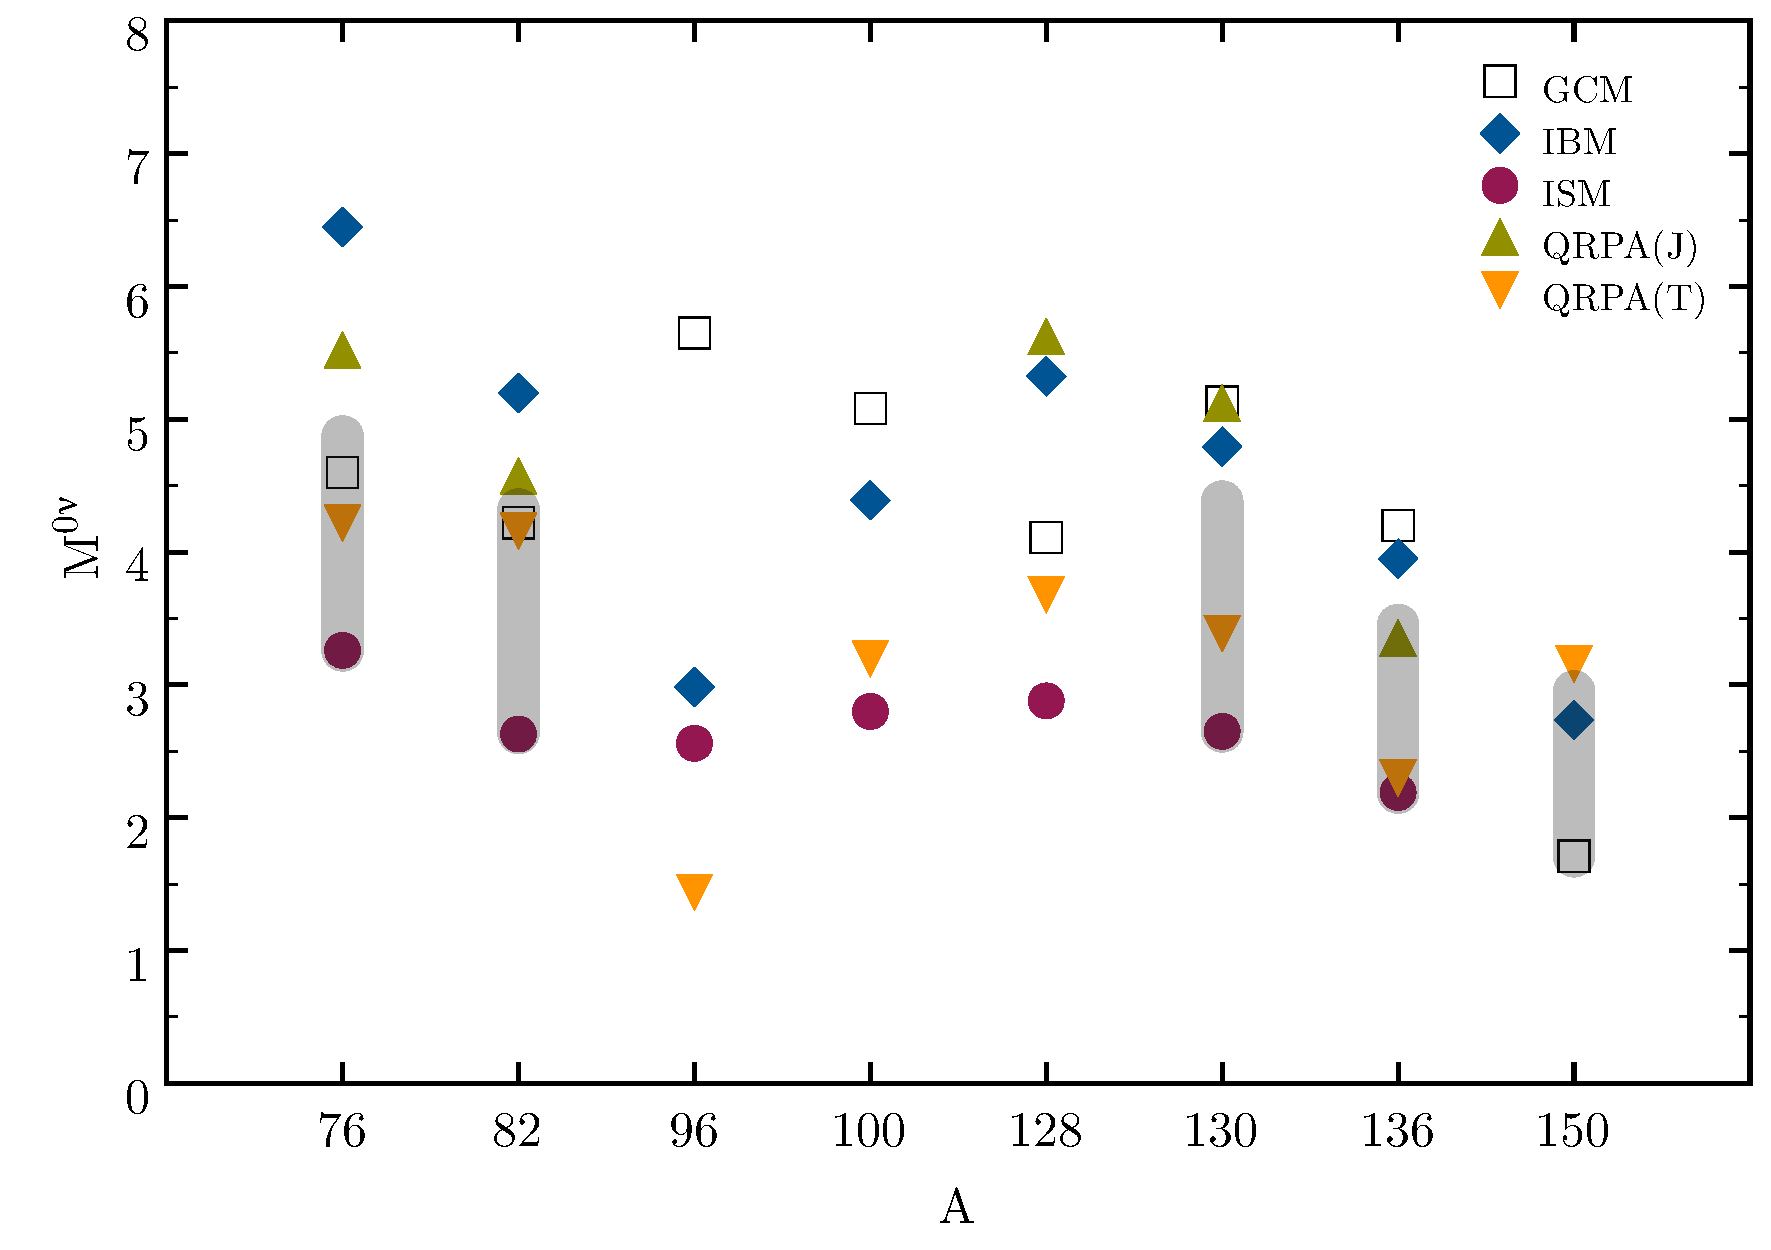
\includegraphics[keepaspectratio=true,width=\textwidth]{SenseAndSensitivityNME.pdf}
\end{center}
\renewcommand{\baselinestretch}{1}
\small\normalsize
\begin{quote}
\caption{Nuclear matrix element calculations for a variety of isotopes.  The behavior is relatively stable from isotope to isotope due to the short-range interaction for $\beta\beta 0\nu$ decay.  Figure from~\cite{1475-7516-2011-06-007}.}
\label{fig:MatrixElementComparisonVsAtom}
\end{quote}
\end{figure}
\renewcommand{\baselinestretch}{2}
\small\normalsize

The nuclear matrix element $M_{0\nu}$ describes the transition rate from the initial to the final nuclear state of the decay process.  The transition may be treated as a two-step process:
\begin{align}
(Z,A) &\rightarrow (Z+1,A) + e^{-} + \bar{\nu}_e \notag \\
\nu_e + (Z+1,A) &\rightarrow (Z+2,A) + e^{-},
\end{align}
where the intermediate state is a virtual state because it does not conserve energy.  Because the two converted protons must be near each other within the nucleus for the neutrino interaction to occur, the $M_{0\nu}$ is not very sensitive to the variations in nuclear structure between elements; this is in contrast to the transition probability for $\beta\beta 2\nu$, $M_{2\nu}$, for which the neutrons may be well-separated within the nucleus~\cite{PetrVogel0nuAnd2nuMatrixElements}.  This similarity can be observed in figure~\ref{fig:MatrixElementComparisonVsAtom}.

%The three components to a nuclear matrix calculation are:
%\begin{itemize}
%\item Computation of the ground-state nuclear structure of the initial nucleus.
%\item Computation of the ground-state nuclear structure of the final nucleus.
%\item Evaluation of the $\beta\beta 0\nu$ transition operator.
%\end{itemize}
%All three of these components can only be performed approximately, and the choice of approximations accounts for differences up to a factor of 2-3 between matrix element calculations~\cite{RMPbb0n}.  Some of the available choices are outlined here.

To compute the nuclear matrix elements $M_{0\nu}$, two main approaches exist: the quasi-random phase approximation (QRPA) and the nuclear shell model.  In the simpler random phase approximation (RPA), the transition from initial to virtual intermediate state and from intermediate to final state are produced by operators of the form $p^+ n$, where $p^+$ represents the proton creation operator and $n$ represents the neutron annihilation operator.  The goal is to make these operators more bosonic (and hence more amenable to treatment in a statistical fashion), and so these operators are diagonalized in a new basis which acts on pairs of nuclei and obeys bosonic commutation rules.  QRPA is similar to RPA, but additionally takes into account the preference of like nuclei to pair together.  This is accomplished at the cost of breaking nucleon number conservation in the operator, but nucleon number is still preserved on average, and the modification can have a significant impact on the result~\cite{RMPbb0n}.

The other common approach to nuclear matrix calculations, the nuclear shell model, attempts to capture more fully the dynamics of a nuclear system by including the full nucleon state space and using nucleon-pair (or higher-order) interactions which can be measured empirically from small nuclei.  The disadvantage compared to QRPA is its enormous computational demands which make a full shell model treatment of relevant $\beta\beta 0\nu$ nuclei impossible at this point.  However, it is possible to perform nuclear shell model calculations with a severely truncated state space, and for nuclei whose shape is close to spherical the results can be reasonable.  As computational power increases it is likely that the shell model will overtake QRPA methods, but for now only a few large-scale shell model calculations of $\beta\beta 0\nu$ matrix elements have been undertaken~\cite{RMPbb0n}.

One important component of both the shell model and QRPA techniques is feedback from experimental data.  This can serve two purposes.  The first is validation: because both approaches make significant approximations, the results of those approximations must generally be tested empirically to ensure they do not have adverse consequences for the accuracy of the result.  Observables such as nuclear energy levels and emission spectra are commonplace; only recently, however, have precision decay rates for $\beta\beta 2\nu$ decay begun to appear in the literature~\cite{bb2nEXO2014}.  Although there are many differences between the calculations of $M_{2\nu}$ and $M_{0\nu}$, still it is currently the best source of validation for $M_{0\nu}$ calculations available, so this can help researchers to improve their understanding of the appropriate approximations for double-beta decay matrix elements.

The other benefit of experimental data is that it can help to constrain input parameters to the calculations.  In QRPA, a parameter called $g_{pp}$ controls the strength of phonon-phonon interactions and needs to be fixed from experimental data; the double-beta matrix elements depend strongly on the value of this parameter, and precision observations of $\beta\beta 2\nu$ can be used to constrain its value~\cite{RMPbb0n,PetrVogel0nuAnd2nuMatrixElements}.  In the shell model, the extreme truncation of the single-particle state space results in a need to renormalize the axial vector current $g_A$, which requires a related observable to control that renormalization; precision observations of $\beta\beta 2\nu$ can be an appropriate method to constrain that value as well.  One disadvantage to the use of $\beta\beta 2\nu$ decay rates to constrain parameters which are input to calculations is that the same observations can no longer be used to validate the approximations for double-beta decays~\cite{PetrVogel0nuAnd2nuMatrixElements}.  A description of efforts to obtain new experimental data useful for nuclear theory can be found in \cite{ZuberWorkshop}.

When the results from modern shell model and QRPA calculations are compared, it is found that the results can differ by as much as a factor of 2-3~\cite{RMPbb0n}.  Provided that there is no systematic effect which impacts both methods similarly, this permits us to understand in a rough way the level of accuracy provided by these calculations.  Progress in reducing these differences continues primarily by increasing the number of single-particle states that can be included, but it is clear that for the near term the search for $\beta\beta 0\nu$ will only be able to set rough limits on Majorana neutrino mass.

\section{Neutrino Flavor Physics}\label{sec:NeutrinoFlavorPhysics}

Neutrinos are known to exist in three flavors, or eigenstates which are diagonal with respect to the lepton interaction terms of the Standard Model.  These flavors are $\nu_e$, $\nu_\mu$, and $\nu_\tau$; they interact, respectively, with $e$, $\mu$, and $\tau$ leptons.  We also expect there to be a basis in which the neutrino mass matrix is diagonalized, and these two bases are not the same.  We call the mass eigenstates $\nu_1$, $\nu_2$, and $\nu_3$ with respective masses $m_1$, $m_2$, and $m_3$.  The unitary operator which translates between the two bases is specified by:
\begin{equation} \label{eqn:ShortDefinitionOfU}
\begin{pmatrix} \nu_e \\ \nu_\mu \\ \nu_\tau \end{pmatrix}
=
\mathbf{U}
\begin{pmatrix} \nu_1 \\ \nu_2 \\ \nu_3 \end{pmatrix}
=
\begin{pmatrix}
U_{e1} & U_{e2} & U_{e3} \\
U_{\mu1} & U_{\mu2} & U_{\mu3} \\
U_{\tau1} & U_{\tau2} & U_{\tau3}
\end{pmatrix}
\begin{pmatrix} \nu_1 \\ \nu_2 \\ \nu_3 \end{pmatrix}.
\end{equation}

These formalities are uninteresting if the neutrino sector is massless, since the mass eigenstates are degenerate.  However, in the case where neutrinos are massive, we can see that neutrinos which are created in one flavor eigenstate will oscillate between the flavor eigenstates with a period which depends on the differences between masses, as is typical in an N-state quantum system.  In the neutrino sector, we can more specifically state that the probability for a transition from flavor $\alpha$ to flavor $\beta$ will be:~\cite{RevModPhys.75.345}
\begin{equation}
P_{\alpha \beta} = \delta_{\alpha \beta} - 4 \sum_{i=1}^2 \sum_{j=i+1}^3 Re \left[ U_{\alpha i} U^{*}_{\beta i} U^{*}_{\alpha j} U_{\beta j} \right] sin^2 \left( \frac{ \left[m_i^2 - m_j^2\right]L}{4E} \right)
\end{equation}
where $L$ is the distance (or time, in $c=1$ units) between neutrino source and destination, and $E$ is the relativistic energy of the emitted neutrinos.

The transition probability is sensitive to the masses of the neutrinos, but only in the form $\left| m_i^2 - m_j^2\right|$.  These measurements have now been performed in a variety of neutrino oscillation experiments, and the best current constraints are $\left| m_1^2 - m_2^2 \right| = (7.50 \pm 0.20) \cdot 10^{-5} \text{eV}^2$~\cite{PhysRevD.83.052002} and $\left| m_2^2 - m_3^2 \right| = 2.32^{+0.12}_{-0.08} \cdot 10^{-3} \text{eV}^2$~\cite{PhysRevLett.106.181801}.

However, oscillation experiments cannot constrain the overall mass scale of neutrinos; they can only set a conservative lower limit that $max(m_2, m_3) \ge 0.048$ eV if we assume one of $m_2$ or $m_3$ is zero.  Furthermore, they do not establish the sign of the difference.  We can see that $m_1$ and $m_2$ are fairly close together, and $m_3$ is significantly different; but we cannot see whether $m_3$ is larger or smaller than the other two masses.  We refer to the situation with $m_1 \simeq m_2 \ll m_3$ as the normal hierarchy, and $m_3 \ll m_1 \simeq m_2$ as the inverted hierarchy; the regime where $m_1 \simeq m_2 \simeq m_3 \gg \left| m_2^2 - m_3^2 \right|$ is called the degenerate region.  Distinguishing between these three situations is one of the significant open questions in neutrino physics because of its impact on observable quantities.

\section{Particle Physics Constraints}\label{sec:ParticlePhysicsConstraints}

To produce more detailed constraints on neutrino physics, it is generally useful to provide a parametrization of the mixing matrix $\mathbf{U}$ from equation~\ref{eqn:ShortDefinitionOfU}.  The standard parametrization is:
\begin{align} \label{eqn:LongDefinitionOfU}
  \mathbf{U} &=
    \begin{pmatrix}
    U_{e1} & U_{e2} & U_{e3} \\
    U_{\mu1} & U_{\mu2} & U_{\mu3} \\
    U_{\tau1} & U_{\tau2} & U_{\tau3}
    \end{pmatrix} \notag \\
  &= \begin{aligned}[t]
      \begin{pmatrix}
      1 & 0 & 0 \\
      0 & cos(\theta_{23}) & sin(\theta_{23}) \\
      0 & -sin(\theta_{23}) & cos(\theta_{23})
      \end{pmatrix}
      \begin{pmatrix}
      cos(\theta_{13}) & 0 & sin(\theta_{13})e^{-i\delta} \\
      0 & 1 & 0 \\
      -sin(\theta_{13})e^{i\delta} & 0 & cos(\theta_{13})
      \end{pmatrix} \times \\
      \begin{pmatrix}
      cos(\theta_{12}) & sin(\theta_{12}) & 0 \\
      -sin(\theta_{12}) & cos(\theta_{12}) & 0 \\
      0 & 0 & 1
      \end{pmatrix}
      \begin{pmatrix}
      e^{i\alpha_1/2} & 0 & 0 \\
      0 & e^{i\alpha_2/2} & 0 \\
      0 & 0 & 1
      \end{pmatrix}.
    \end{aligned}
\end{align}
Out of the six parameters used in defining this matrix, the only ones which have been measured are the three mixing angles $sin^2(2\theta_{12}) = 0.857^{+0.023}_{-0.025}$~\cite{PhysRevD.83.052002}, $sin^2(2\theta_{13}) = 0.089 \pm 0.010 \text{(stat)} \pm 0.005\text{(sys)}$~\cite{1674-1137-37-1-011001}, and $sin^2(2\theta_{23}) > 0.95$~\cite{PhysRevLett.107.241801}.  The Dirac phase $\delta$ is in principle observable from oscillation experiments, but no current experiments have achieved the sensitivity necessary to accomplish this.  The Majorana phases $\alpha_1$ and $\alpha_2$ cannot be extracted from neutrino oscillations~\cite{RMPbb0n}.

The sum of the three mass eigenstates, $M = \sum m_i$, can be constrained by cosmological observations.  This constraint, like all cosmologically-based constraints, is model-dependent; it relies on the expectation that low-mass, hot forms of dark matter similar to neutrinos promote the formation of large-scale structures in the early universe by allowing extremely remote regions of matter to remain in thermal equilibrium.  Recent results from Planck combined with WMAP and baryon acoustic oscillations have restricted $M < 0.230$ eV with $95\%$ confidence~\cite{CosmologicalLimits}.  Considering the assertion in section~\ref{sec:NeutrinoFlavorPhysics} that the heaviest neutrino must have a mass no less than $0.048$ eV, we can see that this cosmological constraint pushes $M$ to within a factor of five of its lower limit. Taken at face value, the Planck measurement is the strongest existing constraint on the absolute mass scale of neutrinos.

Closer to home, the mass of neutrinos is also reflected in $\beta$ decay, $d \rightarrow u + e^- + \bar{\nu}_e$.  The total energy of the daughter products is known, and is shared between the electron and antineutrino; the minimum energy of the antineutrino is its rest mass, so by searching for the maximum energy of the electron we can simultaneously measure the rest mass of the neutrino.  The electron anti-neutrino emitted from beta decay is a mixture of all three mass eigenstates; since no current or planned experiment has sufficiently good energy resolution to resolve the separate endpoints from the three neutrino masses, we can instead write an effective rest mass of an electron antineutrino as:~\cite{RMPbb0n}
\begin{equation} \label{eqn:DefinitionOfMBeta}
\left< m_\beta \right>^2 = \sum_i m_i^2 \left| U_{ei} \right|^2.
\end{equation}

\begin{figure}
\begin{center}
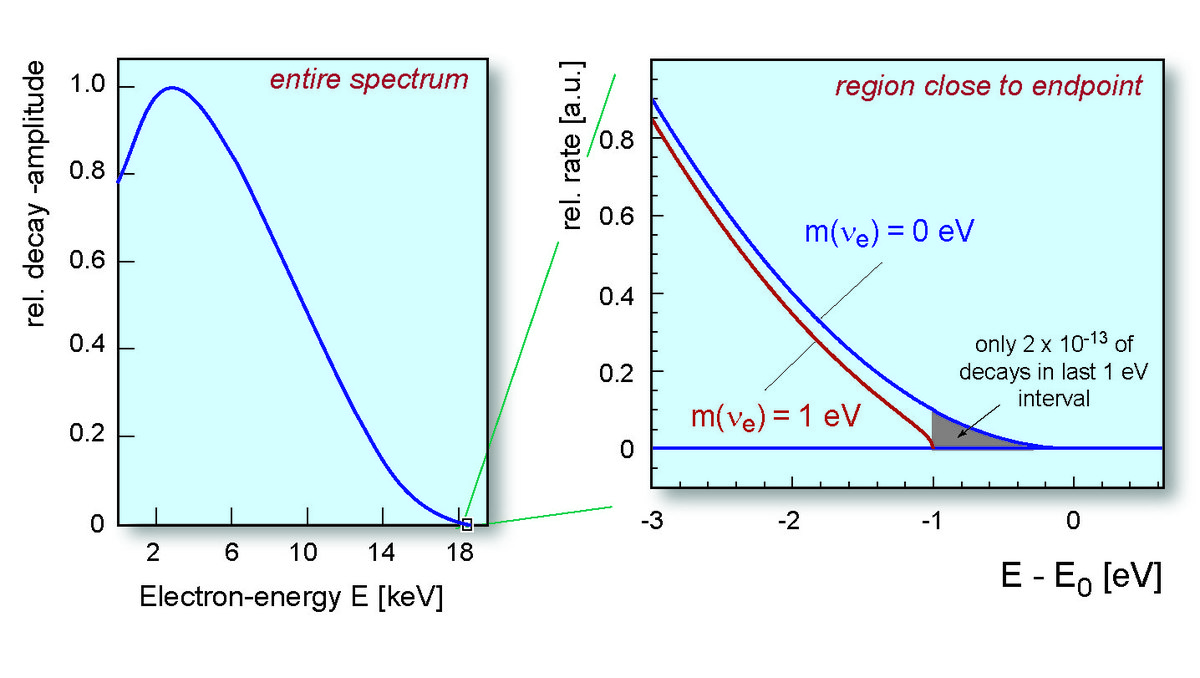
\includegraphics[keepaspectratio=true,width=\textwidth]{TritiumSpectrum.jpg}
\end{center}
\renewcommand{\baselinestretch}{1}
\small\normalsize
\begin{quote}
\caption{The electron spectrum of Tritium ($^3H$) $\beta$ decay.  The endpoint contains only a small fraction of the total statistics.  Figure from~\cite{Angrik:2005ep}.}
\label{fig:TritiumSpectrum}
\end{quote}
\end{figure}
\renewcommand{\baselinestretch}{2}
\small\normalsize

To measure $\left< m_\beta \right>$ we must observe the electron energy spectrum of beta decays at the endpoint, which is complicated by the fact that this portion of the electron spectrum contains only a small fraction of the total electron statistics.  Tritium ($^3H$) is commonly used for these experiments because it has a medium-length halflife of $12.3$ years and an extremely low $\beta$ decay endpoint energy of $18.6$ keV, which maximizes the relative shift in endpoint energy due to $\left< m_\beta \right>$.  Figure~\ref{fig:TritiumSpectrum} shows that for $\left< m_\beta \right> = 1$ eV in Tritium, experiments must observe a shift in the spectrum which affects only about one decay in $5 \cdot 10^{12}$, making this level of sensitivity extremely difficult to achieve.  The best existing limit from $\beta$ decay is $\left<m_\beta\right> < 2.05$ eV, with $95\%$ confidence, from the Troitsk experiment which ran from 1994 to 2004~\cite{OldTritium}.  The KATRIN experiment hopes to achieve a sensitivity of $0.2$ eV, and is expected to begin taking data in 2015~\cite{NewTritium,NewTritiumTimeline}.

\section{Nuclear Physics Constraints from \texorpdfstring{$\beta\beta 0\nu$}{Neutrinoless Double-Beta}}\label{sec:NucPhysConstraintsFromBB0N}

As stated in equation~\ref{eqn:HalfLifeMatrixElementEqn}, it is possible to relate the rate of $\beta\beta 0\nu$ decay to the effective Majorana neutrino mass $\left< m_{\beta\beta} \right>$ by:
\begin{equation}\label{eqn:HalfLifeMatrixElementEqn_thelatter}
\left[T^{0\nu}_{1/2}\right]^{-1} = G_{0\nu}(Q_{\beta\beta}, Z) \left| M_{0\nu}\right|^2 \left< m_{\beta\beta} \right>^2,
\end{equation}
where the phase-space factor $G_{0\nu}(Q_{\beta\beta}, Z)$ and nuclear matrix element $M_{0\nu}$ have been described in section~\ref{sec:NuclearMatrixCalculations}.  We can now proceed to relate the effective Majorana neutrino mass to the parametrization of section~\ref{sec:NeutrinoFlavorPhysics}.  We follow this relation with a discussion of the considerations which affect a $\beta\beta 0\nu$ decay search and a summary of the current state of the field.

The effective Majorana neutrino mass $\left< m_{\beta\beta} \right>$ comes from a combination of the three mass eigenvalues described in section~\ref{sec:NeutrinoFlavorPhysics}.  It takes the form:
\begin{equation} \label{eq:DestructiveMassInteraction}
\left< m_{\beta\beta} \right> = \left|\sum_k m_k U_{ek}^2\right|.
\end{equation}
Unlike $\left< m_\beta \right>$, which is an incoherent sum of strictly positive terms in equation~\ref{eqn:DefinitionOfMBeta}, we can see that $\left< m_{\beta\beta} \right>$ is a coherent sum of terms, each of which may have arbitrary complex phase which may increase or decrease the result of equation~\ref{eq:DestructiveMassInteraction}.  In other words it is possible, even if neutrinos do have Majorana mass, for $\left< m_{\beta\beta} \right>$ to be arbitrarily small if $\mathbf{U}$ is tuned to produce cancellations between terms, specifically by tuning the Majorana phases and selecting the normal rather than inverted mass hierarchy~\cite{PDG}.

\begin{figure}
\begin{center}
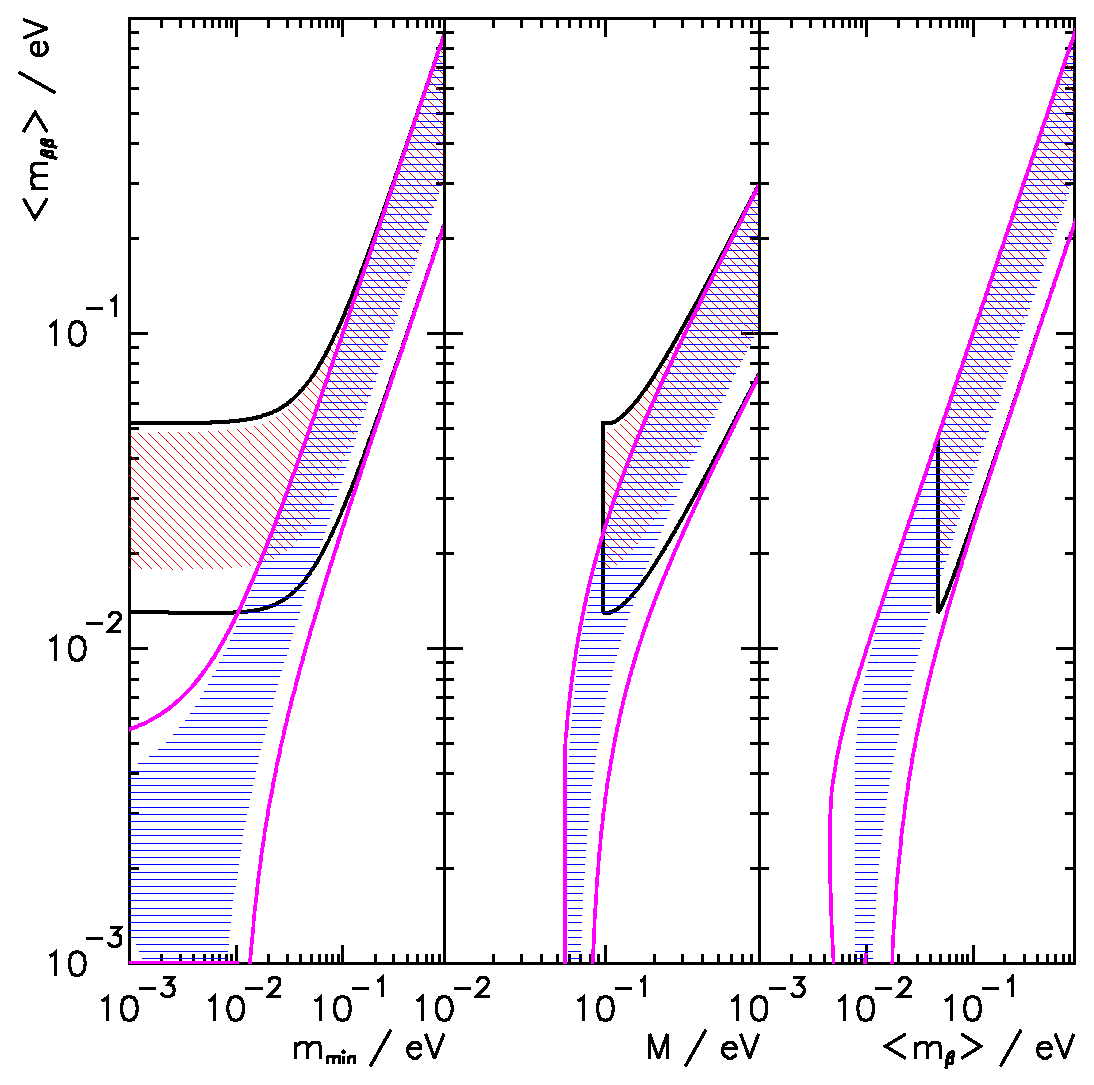
\includegraphics[keepaspectratio=true,width=\textwidth]{PDGNeutrinoMassBounds.eps}
\end{center}
\caption{The relationship between the effective Majorana mass $\left<m_{\beta\beta}\right>$ and other fundamental neutrino quantities: the lightest neutrino mass eigenstate $m_{min}$, the sum of mass eigenstates $M = \sum m_i$, and the effective single-beta-decay neutrino mass $\left<m_{\beta}\right>$.  Black (magenta) lines indicate the allowed region for the inverted (normal) hierarchy; red (blue) hatches indicate uncertainty for the inverted (normal) hierarchy due to the unknown CP-violating and Majorana phases $\delta$, $\alpha_1$, and $\alpha_2$~\cite{PDG}.}
\label{fig:NeutrinoMassBounds}
\end{figure}

It is possible to relate the observables $\left< m_{\beta\beta} \right>$, $\left< m_\beta \right>$, and $M$ within the model for $\mathbf{U}$ of equation~\ref{eqn:LongDefinitionOfU}.  These relations are shown in figure~\ref{fig:NeutrinoMassBounds}; we recall from section~\ref{sec:ParticlePhysicsConstraints} that beta spectrum measurements constrain $\left<m_\beta\right> < 2.05$ eV and cosmological observations constrain $M < 0.230$ eV, both with $90\%$ confidence.  The strongest constraints on $\left<m_{\beta\beta}\right>$ from $\beta\beta 0\nu$ searches place $\left<m_{\beta\beta}\right> < 0.15-0.4$ eV, depending on the choice of matrix element calculations.  We can see that if the cosmological limits are to be trusted, they provide the strongest constraints on the neutrino mass parameters; however, all three observables are complementary, and the wide range of experimental approaches means that systematic effects are unlikely to be shared by all three methods.  The figure shows the relation between these parameters in blue for the normal hierarchy and red for the inverted hierarchy; we note that it is only for the normal hierarchy at equation~\ref{eq:DestructiveMassInteraction} can lead to an extremely small $\left< m_{\beta\beta} \right>$.  In the case of the inverted hierarchy we can see $\left< m_{\beta\beta} \right> > 0.013$ eV, only an order of magnitude lower than the current limits.

The sensitivity of an experiment for measuring $T_{1/2}^{0\nu}$ can be described by the approximate formula:~\cite{RMPbb0n}
\begin{equation}\label{eqn:ApproxHalflifeSensitivity}
T_{1/2}^{0\nu}(n_\sigma) = \frac{4.16 \cdot 10^{26} yrs}{n_\sigma} \left( \frac{\epsilon a}{W}\right) \sqrt{\frac{Mt}{b \Delta E}},
\end{equation}
where $M$ is the mass of material, $a$ is the isotopic enrichment, $W$ is the molecular mass of the material in atomic units, and $t$ is the live-time of the experiment; $\epsilon$ is the signal efficiency, $b$ is the background rate (in counts per kg keV year, or some similar units), and $\Delta E$ is the energy resolution of the detector at the $Q$-value; and $n_\sigma$ is the desired confidence limit, in sigmas, where the standard $90\%$ confidence limit will require $n_\sigma = 1.64$.  The scaling of this equation is most accurate when the energy resolution is much smaller than the $Q$-value and the background is uniformly distributed in energy; however, when combined with phase factor and nuclear matrix element estimates it roughly allows us to compare the sensitivity of different $\beta\beta 0\nu$ experiments.

According to equation~\ref{eqn:ApproxHalflifeSensitivity} we should prefer experiments for which:
\begin{itemize}
\item A large quantity of highly-enriched isotope can be obtained.
\item Signal detection is highly efficient.
\item Background contamination around the $Q$-value is small, and does not scale with detector mass.
\item Good energy resolution can be achieved.
\end{itemize}

The leading experiments which are planned or currently searching for $\beta\beta 0\nu$ are as follows:
\begin{enumerate}
\item The leading search for $^{76}$Ge comes from the GERDA experiment at the Gran Sasso Laboratory in Italy.  GERDA consists of an array of cryogenic germanium detectors with charge readout.  $^{76}$Ge has a $Q$-value of only 2039 keV, giving it a lower phase factor than other popular materials.  It also is expensive to grow large uniform crystals of germanium; this means that it is difficult for a germanium experiment to take advantage of self-shielding from external radioactive backgrounds.  However, its strongest advantage is its excellent energy resolution: GERDA has achieved an energy resolution at its $Q$-value of 1.1-1.7 keV ($\sigma$) with its newer crystals~\cite{PhysRevLett.111.122503}.
\item The best results with $^{130}$Te have come from the CUORICINO experiment which ran at the Gran Sasso Laboratory in Italy.  CUORICINO was a bolometric experiment: it cooled tellurium crystals to extremely low temperatures where the heat capacity becomes small, so that a decay inside the tellurium creates a measurable change in temperature.  Similarly to $^{76}$Ge, it is expensive to grow large crystals of tellurium, so most tellurium experiments use an array of detectors.  $^{130}$Te has a $Q$-value of 2528 keV, somewhat larger than that of $^{76}$Ge, but the energy resolution of the enriched crystals was 2.1-10.6 keV ($\sigma$), depending on the crystal.  CUORICINO stopped running in 2008~\cite{Andreotti2011822}; planned experiments in $^{130}$Te include CUORE~\cite{1402.0922} and SNO+~\cite{1402.1170}, both of which anticipate data-taking beginning in 2015.
\item The two leading experiments in $^{136}$Xe are KamLAND-Zen, located at the Kamioka Observatory, and EXO-200, located in the WIPP facility.  $^{136}$Xe also has a $Q$-value of 2458 keV, giving it a higher phase-space factor than $^{76}$Ge but not $^{130}$Te.  KamLAND-Zen dissolves its xenon in a liquid scintillator and observes only scintillation energy; it achieves an energy resolution of 103 keV ($\sigma$), modest compared to the resolution achieved in tellurium and germanium, but its monolithic nature allows it to keep backgrounds low~\cite{PhysRevLett.110.062502}.  EXO-200 is a pure liquid xenon detector which observes both ionization and scintillation. This, combined with analysis improvements described in the present work, allows it to achieve a somewhat better energy resolution of 38 keV ($\sigma$)~\cite{NewEXObb0nPaper_2014}.
\end{enumerate}

\begin{table}
\begin{center}
\begin{tabular}{|rccccr|}
\hline Isotope & $T_{1/2}^{0\nu}$ (years) & $M_{0\nu}$ & $G_{0\nu}$ (yrs${}^{-1}$) & $\left<m_{\beta\beta}\right>$ (eV) & Collaboration \\ \hline
$^{48}$Ca & $5.8 \cdot 10^{22}$ & 2.28 & $2.48 \cdot 10^{-14}$ & $3.7$ & ELEGANT IV \cite{ElegantIV}\\
$^{76}$Ge & $2.1 \cdot 10^{25}$ & 5.98 & $2.36 \cdot 10^{-15}$ & $0.24$ & GERDA \cite{PhysRevLett.111.122503} \\
$^{82}$Se & $3.6 \cdot 10^{23}$ & 4.84 & $1.02 \cdot 10^{-14}$ & $1.1$ & NEMO-3 \cite{NEMO2011RandomOtherIsotopes}\\
$^{96}$Zr & $9.2 \cdot 10^{21}$ & 2.89 & $2.06 \cdot 10^{-14}$ & $8.0$ & NEMO-3 \cite{Argyriades2010168}\\
$^{100}$Mo & $1.1 \cdot 10^{24}$ & 4.31 & $1.59 \cdot 10^{-14}$ & $0.56$ & NEMO-3 \cite{NEMO3-2013-100Mo}\\
$^{116}$Cd & $1.6 \cdot 10^{22}$ & 3.16 & $1.67 \cdot 10^{-14}$ & $6.1$ & NEMO-3 \cite{NEMO2011RandomOtherIsotopes}\\
$^{130}$Te & $3.0 \cdot 10^{24}$ & 4.47 & $1.42 \cdot 10^{-14}$ & $0.34$ & Cuoricino \cite{PhysRevC.78.035502}\\
$^{136}$Xe & $1.1 \cdot 10^{25}$ & 3.67 & $1.46 \cdot 10^{-14}$ & $0.22$ & EXO-200 \cite{NewEXObb0nPaper_2014}\\
$^{136}$Xe & $1.9 \cdot 10^{25}$ & 3.67 & $1.46 \cdot 10^{-14}$ & $0.16$ & KamLAND-Zen \cite{PhysRevLett.110.062502}\\
$^{150}$Nd & $1.8 \cdot 10^{22}$ & 2.74 & $6.30 \cdot 10^{-14}$ & $3.4$ & NEMO-3 \cite{PhysRevC.80.032501}\\
\hline
\end{tabular}
\end{center}
\caption{A listing of the strongest available $\beta\beta 0\nu$ limits; all half-life and mass limits are quoted at $90\%$ confidence.  Limits on $\left<m_{\beta\beta}\right>$ are obtained using phase space factors from~\cite{PhysRevC.85.034316} and matrix elements from~\cite{PhysRevLett.109.042501}, both chosen for the completeness of their tabulations.  These sources explicitly factor out $g_A$; we use $g_A = 1.269$.  For $^{136}$Xe, both Kamland-Zen's published results and the EXO-200 results described in this work are included in the table.}
\label{tab:0nubb_limits}
\end{table}

Table~\ref{tab:0nubb_limits} tabulates the most current $T_{1/2}^{0\nu}$ limits in all $\beta\beta 0\nu$ isotopes for which $\beta\beta 0\nu$ limits have been published.  Representative limits on $\left< m_{\beta\beta}\right>$ are also included; these come from one particular set of phase space factors and nuclear matrix element calculations performed using the interacting-boson model; this pair of sources for calculations is made because they include tabulations for a broad range of isotopes and permit comparisons across all available half-life limits~\cite{PhysRevC.85.034316,PhysRevLett.109.042501}.  However, one should bear in mind that errors in the matrix elements propagate to errors in $\left< m_{\beta\beta}\right>$ of as much as a factor of two for each isotope.  We can see that although there are a favored set of isotopes, active and successful programs exist in a wide range of isotopes, and no one isotope is ideal in all respects.

As the table indicates, $^{136}$Xe has provided some of the strongest constraints on $\left< m_{\beta\beta}\right>$ in spite of its relatively modest energy resolution.  The present work demonstrates significant improvements to the energy resolution observed by the EXO-200 detector in $^{136}$Xe which have been achieved through offline denoising of the scintillation signals.  This denoising technique is applied to data from the detector, and results in a stronger limit on $T_{1/2}^{0\nu}$ from EXO-200 than could be obtained from the same data without denoising.  Chapter~\ref{ch:DenoisingResults} presents recent results from EXO-200 which benefit from this denoising technique, as well as increased livetime and other improvements.

\renewcommand{\thechapter}{2}
\chapter{The EXO-200 Detector}

Among the experiments with potential to match the sensitivity of Heidelberg-Moscow is the Enriched Xenon Observatory (EXO).  In particular, the EXO-200 detector is designed to hold 200 kg of Xe enriched to 80\% in $^{136}$Xe, and anticipates probing down to $\left< m_{\beta\beta} \right> \sim 0.1$ eV~\cite{CarterICHEP}.  Xenon is a convenient material to study because it is a noble element, making it easy to purify chemically.  It has no long-lived radioactive isotopes, so there is no concern of cosmogenic activation of the Xenon while aboveground.  It has a fairly high Q-value of 2.458 MeV, giving it a larger phase-space for its decay products and putting its peak out of reach of many common backgrounds.  Xenon also provides two means to measure energy from a decay:  under the influence of an electric field, ionization charge in pure Xenon will drift; and regardless of electric field, excited Xenon scintillates.  The ratio of scintillation to ionization depends on electric field and the density of the energy deposit; thus, at high enough electric field discrimination is possible between high-energy-density $\alpha$-decay and lower-energy-density $\beta$- and $\gamma$-decay.  Another benefit of Xenon is that, since it can act as an energy detector in its pure gaseous or liquid state, it is easy to make a large monolithic Xenon detector.  We will here review how the EXO-200 experiment has been constructed to exploit these properties and explore down to interesting neutrino masses.

\begin{figure}
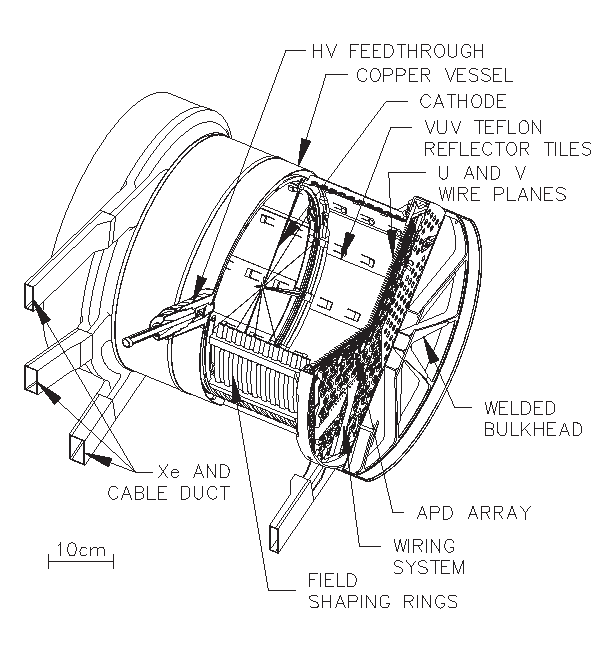
\includegraphics[scale=0.85]{TPCSchematic.eps}
\caption{Schematic of the inner EXO-200 TPC.}
\label{fig:TPCSchematic}
\end{figure}

The core of the EXO-200 detector is a cylindrical time-projection chamber (TPC), depicted in Figure~\ref{fig:TPCSchematic}, under a potential of roughly 400 V/cm.  The electric field is shaped to be parallel to the axis of the TPC throughout its fiducial volume.  The cathode is located in the middle of the TPC, and charge is collected on grids of parallel wires on either end of the TPC, giving a high-quality probe of the total ionization charge and location along one axis.  Also on both ends of the TPC, in front of these collection wires is another grid of parallel wires, orthogonal to the collection wires, which identifies an induced signal from passing ionization charge to give another position coordinate.  Finally, on both endcaps of the TPC are many large-area avalanche photodiodes (LAAPDs) which can detect the scintillation light from the primary decay~\cite{EXOLAAPD}.  The time difference between scintillation and charge collection gives a third position coordinate from a decay, and the scintillation also can give a secondary measurement of the energy of the deposit.  As noted above, comparing the scintillation and collected ionization allows $\alpha$-decays to be identified, removing one broad source of backgrounds.

The Xenon must be kept extremely pure, both to reduce backgrounds and to permit the ionization charges to drift farther with less attenuation.  To accomplish this, the detector has two pipes feeding into it so that Xenon may be circulated out of the detector continuously for repurification.  This is done using SAES Zirconium getters, which filter out all chemically reactive elements and return only noble elements.  Radioactive isotopes which are not filtered out are $^{85}$Kr (which has a Q-value much lower than that of $^{136}$Xe, making it fairly harmless) and all forms of Radon (some of whose daughter products can deposit energy around the Q-value of $^{136}$Xe).

The TPC itself is made of oxygen-free high-thermal-conductivity (OFHC) copper that was kept under concrete shielding during its time aboveground to protect it from neutron-induced activation.  Nevertheless, the copper may be a significant source of backgrounds in the energy range of interest, primarily due to natural contamination by $^{40}$K, $^{238}$U and $^{232}$Th~\cite{MaterialsCatalog}.  To mitigate this, significant effort has been expended in making the copper walls as thin as possible, averaging $1.5$ mm thick.  The ductility of copper makes such thin walls technically challenging, and a significant infrastructure has been developed to maintain the pressure of ultrapure HFE coolant, in which the TPC is immersed, so that the pressure difference can be controlled to $\sim 10$ torr.

Other significant sources of background may be the charge collection wires that pass through the TPC and the LAAPDs on its ends.  Both backgrounds have been minimized by limiting the total mass and carefully selecting materials to use.  The charge collection wires are photo-etched from phosphor bronze; the etching process was found to contribute to surface contamination, which was minimized by the use of clean etching agents and the use of a more aggressive cleaning procedure after etching~\cite{MaterialsCatalog}.  The LAAPDs are designed to minimize the radioactive contamination they introduce.  They were designed without standard ceramic encapsulation; instead the LXe is itself relied upon to insulate them.  Additionally, Aluminum used in the LAAPDs was found to be high-background, and was replaced with an acceptable substitute.  These efforts have reduced the activity introduced by the LAAPDs~\cite{MaterialsCatalog}\cite{EXOLAAPD}.

These are a few of the critical subsystems that were screened prior to use.  More details will be presented in a forthcoming detector paper to be written by the EXO collaboration.


\renewcommand{\thechapter}{4}
\chapter{Denoising Theory}

As has been discussed, the performance of double-beta experiments like EXO-200 is partially determined by their energy resolution.  In EXO-200, the energy resolution is limited by the scintillation energy resolution, which in turn is dominated by electronic noise in the APDs.  Significant effort must therefore be expended to understand and reduce the noise in the scintillation signals.

\begin{figure}
\begin{center}
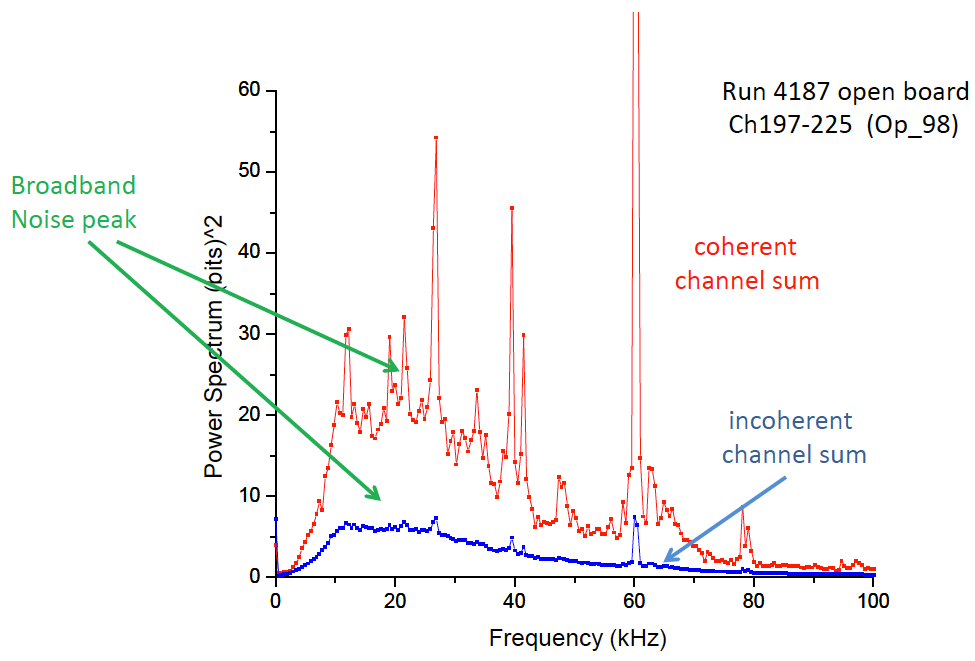
\includegraphics[keepaspectratio=true,width=\textwidth]{APDNoisePowerSpectrum.png}
\end{center}
\renewcommand{\baselinestretch}{1}
\small\normalsize
\begin{quote}
\caption{Coherent and incoherent noise power spectra for a sample set of APD channels without signal shaping.~\cite{ElectronicsUpgradeReport}}
\label{fig:APDNoisePowerSpectrum}
\end{quote}
\end{figure}
\renewcommand{\baselinestretch}{2}
\small\normalsize

When the noise in the APDs is studied, it was found that the individual APD channels met targetted root-mean-square noise levels of 2000 electrons.  However, rather than observing the noise on summed APD channels increase proportionally to the square root of the number of channels, the summed APD noise is roughly two to three times higher than projected.  This worse-than-expected scaling of the noise with channels indicates that noise across different channels is correlated, and further analysis confirms that the bulk of the noise on an unshaped APD waveform is correlated with other channels, as shown in Figure~\ref{fig:APDNoisePowerSpectrum}.  There are many possible sources of coherent noise in the hardware, and reducing the amount of coherent noise is a topic for further research.~\cite{ElectronicsUpgradeReport}

However, the observation that coherent noise is the dominant source of noise in the APDs, and thus also the limiting factor in EXO-200's energy resolution, means that it should be possible to exploit these correlations and reduce the level of noise in offline analysis.  This chapter will describe a scheme to accomplish that goal and produce an optimal estimate of scintillation energy which takes noise correlations into account.

It is worth noting that in fact there are a number of different qualitative approaches to reducing the noise levels in the scintillation channel.  In casual terms, we will refer to "passive" approaches as those in which components of our signals are weighted more or less heavily based on their relative signal-to-noise content.  "Active" approaches, by contrast, will be classified as those which attempt to improve the signal-to-noise content of signal components.  We have identified the following three types of denoising:
\begin{description}
\item[Frequency weighting] \hfill \\
On a given channel signal, weight more heavily the frequency components which contain larger signal-to-noise ratio.  This passive denoising scheme requires knowledge of the shapes in fourier space of a signal and the power spectrum of the noise.

\item[Channel weighting] \hfill \\
Different channels may have different levels of noise, so some may generally have higher-quality signals.  More importantly, though, the amount of signal on a given channel depends strongly on the proximity of the APD gang to the source of scintillation within the detector.  This passive denoising scheme therefore allows us to weight more heavily the channels which have more scintillation, provided we can identify these weights on an event-by-event basis.  This requires knowledge of the magnitude of noise on each channel and of the correspondence between event position and signal magnitude on each APD gang; the latter is described by the lightmap, described earlier.

\item[Noise subtraction] \hfill \\
This active form of denoising consists of using correlations between noise on different channels to produce a better estimate of the noise component of signals than each signal taken independently could provide.  To accomplish this, we will require detailed information about the pairwise noise correlations across channels at each frequency.
\end{description}

In the following, we will describe a general linear operator on the APD signals which in principle can accomplish each of these forms of denoising, and we will presume that all of the described inputs are available; by identifying the parameters for that linear operator which are optimal, we can be confident that the denoising operator we produce will accomplish all three forms of denoising described above.

\section{Setup}

We first establish a number of notational conventions:
\begin{itemize}
\item $i$, $j$ will represent indices over APD channels.
\item $a$, $b$, $c$ will represent indices of signals in an event.
\item $\tau$ will represent the time indices of a discrete waveform; $t_a$ represents the calendar time of a signal $a$.
\item $f$, $g$ will represent the frequency indices of Fourier-transformed waveforms.
\item For a waveform $*[\tau]$, we will represent the discrete Fourier transform of that waveform with $\widetilde{*}[f]$, where the particular convention used to evaluate the Fourier transform is not significant.
\item For a Fourier-transformed waveform $\widetilde{*}[f]$, we denote the real and imaginary parts of that waveform by $\widetilde{*}^R[f]$ and $\widetilde{*}^I[f]$, respectively.
\item For an unknown parameter $*$, the symbol $\widehat{*}$ will identify an estimator for $*$.
\item For an expression $*$ containing random variables, $\left<*\right>$ is the expectation value of $*$.
\end{itemize}

We describe the data as a collection of discretely sampled waveforms, $X_i[\tau]$.  We assume that all signal times and shapes are already known, so we can model the waveforms by $X_i[\tau] = \sum_a M_{ia}Y_{ia}[\tau] + N_i[\tau] + b_i$, where $Y$ is the shape of signal $a$ on channel $i$, $M$ is the magnitude of that signal, and $N$ and $b$ represent the electronic noise and baseline, respectively, of the channel.

To break the degeneracy between $M$ and $Y$, we choose to fix the magnitude of the template signal $Y$.  We choose to require that the signal $Y$ has a magnitude of one, as described in figure~\ref{fig:SampleAPDTemplates}.  This implies that for a typical single-site $2615$-keV deposit, the average values of $M_i$ should be equal to the values of the lightmap $L_i(\vec{x},t)$ described earlier.

Noise correlations will be much simpler in frequency space, so we take the Fourier transform and drop the zero-frequency component to obtain \[\widetilde{X}_i[f] = \sum_a M_{ia}\widetilde{Y}_{ia}[f] + \widetilde{N}_i[f].\]

\section{The Signal Model}

It is first important to characterize the response of the APDs to energy deposits in EXO-200.  This will require us to understand the signal amplification of the detector at each physical stage, as well as the noise introduced by each of these processes.  We will describe both in detail here.

\subsection{APD Noise}

We will assume that there are two sources of noise in this model.  First, the electronic noise $N_i[\tau]$ is assumed to be random.  We require that noise with different frequencies is uncorrelated:
\[\left< \widetilde{N}_i[f] \widetilde{N}_j[g] \right> = 0 \text{~when~} f \ne g.\]
The noise correlations $\left< \widetilde{N}_i[f] \widetilde{N}_j[f] \right>$ are assumed to be known; our means for measuring them are described [ELSEWHERE].

The second random variable will be the magnitude of the signal itself, $M_{ia}$.  When an energetic decay occurs in bulk of the detector, it will release some number of photons.  We will denote the number of photons released by signal $a$ by $P^{(0)}_a$, and this is the parameter we wish to measure.  However, the magnitude signal actually observed on APD channels number of photons actually collected by sensors is a random variable whose distribution depends on $P^{(0)}_a$, and we will now identify the chain of events which produce it.

First, each APD gang $i$ has some number $P^{(1)}_{ia}$ of photons which reach them.  The mean fraction of photons reaching a particular gang $i$ from position $\vec{x}_a$, $f_i(\vec{x}_a)$, is assumed to be known; however, the initial paths of the optical photons emitted from the source, their trajectories through the Xenon, and their success in reflecting off of teflon are all random, so we treat $P^{(1)}_{ia}$ as a Poisson-distributed random variable with mean $f_i(\vec{x}_a)P^{(0)}_a$.  A typical deposit from a $\beta\beta 0\nu$ event may deposit $10-100$ photons on each APD gang [CHECK THIS NUMBER], depending strongly on the location of the deposit; thus, we find that the Poisson noise on a single APD channel may be quite significant.

Additionally, the number of photons reaching different gangs are not uncorrelated; since a photon which reaches gang $i$ cannot deposit on a different gang $j$, $P^{(1)}_{ia}$ and $P^{(1)}_{ja}$ are anticorrelated for different gangs $i \ne j$.  This process is described by a multinomial distribution.  Explicitly, we can identify the expectation values of a multinomial distribution:
\begin{itemize}
\item $\left< P^{(1)}_{ia} \right> = f_i(\vec{x}_a)P^{(0)}_a$
\item $\left< P^{(1)}_{ia} P^{(1)}_{jb} \right> = \left< P^{(1)}_{ia} \right> \left< P^{(1)}_{jb} \right> + \left[ f_i(\vec{x}_a)\delta_{ij} - f_i(\vec{x}_a)f_j(\vec{x}_a) \right] P^{(0)}_a \delta_{ab}$
\end{itemize}

Following the random process associated with photons reaching the APD gangs, there is also randomness associated with signal amplification internally in the APDs.  These processes are described in detail in~\cite{EXOLAAPD}, but we can summarize that:

\begin{enumerate}
\item Optical photons in the liquid xenon arrive at the active layer of the APDs have a wavelength of roughly $178$ nm, meaning that each optical photon has an energy of roughly $7.0$ eV.  The energy required to produce one electron-hole pair in silicon is roughly $3.66$ eV, which means that each incident photon produces roughly $1.9$ electron-hole pairs; we will define $P^{(2)}_{ia}$ to be the number of electron-hole pairs actually produced from $P^{(1)}_{ia}$ incident photons.  The corresponding Fano factor for electrons produced in silicon is roughly $0.1$, meaning that in addition to the uncertainty in $P^{(1)}_{ia}$ which we have already characterized, there is an additional uncorrelated variance in $P^{(2)}_{ia}$ equal to $0.1 \left<P^{(2)}_{ia}\right>$.  The correlations in the parameters $P^{(2)}_{ia}$ are therefore:
\[\left< P^{(2)}_{ia} \right> = 1.9 \cdot P^{(1)}_{ia}\]
\[\left< P^{(2)}_{ia} P^{(2)}_{jb} \right> = (1.9)^2\left< P^{(1)}_{ia} P^{(1)}_{jb} \right> + 0.1 \left< P^{(2)}_{ia}\right> \delta_{ij}\delta_{ab}\]
\item Electron-hole pairs are then amplified by an avalanche process inside the APDs.  The magnitude of this gain is APD-dependent, generally on the order of $200-300$, and can be identified by a time-dependent quantity $G^P_i(t)$; we will call the number of output electrons $P^{(3)}_{ia}$.  In addition to amplification of existing noise in $P^{(2)}_{ia}$, two additional source of noise are introduced.  First, there is statistical variance in the amplification experienced by each electron due to the randomness of the avalanche process.  This variance is dependent on many factors, including the gain, and scales like the square root of the number of electrons; we define the variance on the gain experienced by a single electron as $\sigma^2_{G_i}(t)$.  Second, there are gain non-uniformities in the diode volume, which contribute variance proportional to the square of the number of initial electron-hole pairs; we will identify the proportionality constant as $\sigma^2_{NU}$, which may depend on time and APD gang.  The magnitude of this uncertainty is not well-known, but may be significant.  The correlations in the parameters $P^{(3)}_{ia}$ are therefore:
\[\left< P^{(3)}_{ia} \right> = G^P_i(t_a)P^{(2)}_{ia}\]
\[\left< P^{(3)}_{ia} P^{(3)}_{jb} \right> = G^P_i(t_a)G^P_j(t_b) \left< P^{(2)}_{ia} P^{(2)}_{jb} \right> + \left[P^{(2)}_{ia}\sigma^2_{G_i}(t_a) + \left(P^{(2)}_{ia}\right)^2\sigma^2_{NU}\right]\delta_{ij}\delta_{ab}\]
\end{enumerate}

Finally, there is amplification $G^{E}_i(t)$ associated with the electronics of the APDs which is dependent on time and channel.  This includes preamplifier gain, shaper gain, gain associated with the shaping times, and conversion from voltage to ADC counts.  We assume that no signal-dependent noise is introduced during this stage, but there is constant electronic noise $N_i[\tau]$ which has been described above.  Additionally, the APDs can contribute noise in the form of a dark current which is uncorrelated with signals; this is inseparable from the electronic noise, and so we absorb it into our description of $N_i[\tau]$.

\subsection{APD Signals and Noise}

We have already characterized the overall gain of the APDs using the lightmap described earlier.  We know that a typical single-site deposit of $2615$ keV at position $\vec{x}$ and time $t$ will produce a signal with expected magnitude $L_i(\vec{x},t)$ on APD channel $i$.  We must now connect this empirical understanding of our APD signals with the physical understanding in terms of photons and electrons described above.

We have identified the number of photons created by an event $a$ as $P^{(0)}_a$.  In reality, an ideal scintillation measurement can only measure this quantity, and not the true energy of the event -- there is randomness in the number of photons produced by a known-energy deposit, so $P^{(0)}_a$ will not be perfectly correlated with the energy $E_a$ of the event.  However, the number of photons generated is a difficult parameter to understand empirically, and all of our calibrations occur at a known energy even though the corresponding number of deposited photons is unknown.

Simulations using NEST~\cite{NESTpaper} which have been performed within the EXO group by Liangjian Wen at our bulk electric field indicate that we can expect roughly $82,000$ photons from a $2615$-keV gamma deposit.  We will identify this parameter with $c$, and express the average relation between energy and photon yield in EXO-200 by
$P^{(0)} = c \cdot E$,
where $E$ is the energy measured in units of $2615$ keV.  We will treat this relationship as exact, and attempt to measure $E$ rather than $P^{(0)}$; this means that when we speak of measuring the energy of an event using the APD signals, we really are referring to measuring the "scintillation energy," or a parameter proportional to the number of emitted photons which on average will equal the true energy of the deposit.

Ignoring variances for a moment, we can combine all of the expectation values for numbers of photons or ADC counts above to state that on average,
\[M_{ia} = 1.9 \cdot c f_i(\vec{x}_a) G^P_i(t_a) G^E_i(t_a) E_a.\]
We can compare this to our empirical lightmap measurements, which are expressed by $M_{ia} = L_i(\vec{x}_a,t_a) E_a$,
and we conclude that:
\[ L_i(\vec{x},t) = 1.9 \cdot c f_i(\vec{x}) G^P_i(t) G^E_i(t).\]

We recall that it is assumed the lightmap is a separable function, $L_i(\vec{x},t) = R_i(\vec{x})S_i(t)$, and we can provide the two proportionalities:
\[ R_i(\vec{x}) \propto f_i(\vec{x}) \]
\[ S_i(t) \propto G^P_i(t) G^E_i(t).\]

Although $G^E_i(t)$ is in principle time-dependent, due to environmental effects on the APD electronics and occasional replacement of electronics cards for certain channels, precision data on its value is not readily available.  Instead, we use a time-independent estimate $G^E_i(t) = 1.1 \cdot 10^{-3}$ ADC counts per electron emitted from the APD; the uncertainty in this figure is dominated by uncertainty in the preamplifier gains, which are controlled by a roughly $5$ pF capacitor.  Other contributors to the gain include shaper gain of $21.2$ (from a combination of amplification and shaping) and a full-scale digitizer range of $2.5$ volts for $12$-bit digitization.

We do have independent measurements of the APD gains $G^P_i(t)$ available from laser calibration runs.  These special runs allow a laser to shine into the detector from a fixed point and with a stable amplitude while the bias voltages on the APDs are varied from an effective unity gain to our standard voltage settings.  Using these measurements, we are able to measure $G^P_i(t)$ at weekly intervals from September 2012 to the present time.  Before September 2012, some less-reliable laser data is available, but results from that data are not readily available as of this writing.

It would be possible, and should be a goal for future improvements, to make use of this full range of laser data.  However, the laser data provides a less uniform history of APD gains over the full data-taking window of EXO-200 from September 2011 to November 2013, and it is much easier to track time-dependent behavior from Thorium source data which have been collected regularly throughout that period.  As a result, a compromise is used to characterize $G^P_i(t)$.  One particular laser run, run 4540 (taken on December 13, 2012), is used to fix $G^P_i(t_{4540})$, and the function is extrapolated using Thorium source data with:
\[G^P_i(t) \approx G^P_i(t_{4540}) \cdot S_i(t)/S_i(t_{4540}).\]
This assumption makes use of the approximation that $G^E_i(t)$ is roughly constant in time, which is probably only accurate to one significant figure; therefore when an electronics change is made to a channel, we can expect that the accuracy of $G^P_i(t)$ is no better than one significant figure.  These results mean that we can also estimate with the same level of accuracy:
\[f_i(\vec{x}) \approx \frac{S_i(t_{4540})}{G^P_i(t_{4540})} \cdot \frac{R_i(\vec{x})}{1.9 \cdot c G^E_i(t)}.\]

It is then possible to express the full correlations in signal magnitudes in terms of the scintillation energies of deposits as:
\begin{align*}
\left< M_{ia} \right> &= L_i(\vec{x}_a,t_a) E_a \\
\begin{split}
\left< M_{ia} M_{jb} \right> &= L_i(\vec{x}_a,t_a)L_j(\vec{x}_b,t_b) E_a E_b \left[1 + \frac{\sigma^2_{NU}}{\left(G^P_i(t)\right)^2} \delta_{ij}\delta_{ab} \right] \\
&\quad - L_i(\vec{x}_a,t_a) L_j(\vec{x}_a,t_a) E_a \delta_{ab}/c \\
&\quad + L_i(\vec{x}_a,t_a) G^E_i(t) E_a \delta_{ij} \delta_{ab} \left[\left(0.1 + 1.9\right)G^P_i(t) + \frac{\sigma^2_{G_i}(t)}{G^P_i(t)}\right].
\end{split}\end{align*}
\begin{comment}
THE FOLLOWING IS MY WORK IN EXPANDING THE M_M CORRELATIONS.
IF NEEDED, IT CAN BE UNCOMMENTED AND IS VALID LATEX CODE.

\[ \left< M_{ia} M_{jb} \right> = G^E_i(t) G^E_j(t) \left<P^{(3)}_{ia}P^{(3)}_{jb} \right> \]

\[ \left< M_{ia} M_{jb} \right> = G^E_i(t) G^E_j(t) \left( G^P_i(t)G^P_j(t) \left< P^{(2)}_{ia} P^{(2)}_{jb} \right> + \left[P^{(2)}_{ia}\sigma^2_{G_i}(t) + \left(P^{(2)}_{ia}\right)^2\sigma^2_{NU}\right]\delta_{ij}\delta_{ab}\right)\]

\begin{equation*}\begin{split}
\left< M_{ia} M_{jb} \right> ={}& G^E_i(t) G^E_j(t) G^P_i(t)G^P_j(t) \left< P^{(2)}_{ia} P^{(2)}_{jb} \right> \\
 & + G^E_i(t) G^E_j(t) \left[P^{(2)}_{ia}\sigma^2_{G_i}(t) + \left(P^{(2)}_{ia}\right)^2\sigma^2_{NU}\right]\delta_{ij}\delta_{ab}
\end{split}\end{equation*}

\begin{equation*}\begin{split}
\left< M_{ia} M_{jb} \right> ={}& G^E_i(t) G^E_j(t) G^P_i(t)G^P_j(t) \left( (1.9)^2\left< P^{(1)}_{ia} P^{(1)}_{jb} \right> + 0.1 \left< P^{(2)}_{ia}\right> \delta_{ij}\delta_{ab} \right) \\
 & + G^E_i(t) G^E_j(t) \left[1.9 \cdot P^{(1)}_{ia}\sigma^2_{G_i}(t) + (1.9)^2 \left(P^{(1)}_{ia}\right)^2\sigma^2_{NU}\right]\delta_{ij}\delta_{ab}
\end{split}\end{equation*}

\begin{equation*}\begin{split}
\left< M_{ia} M_{jb} \right> ={}& (1.9)^2 G^E_i(t) G^E_j(t) G^P_i(t)G^P_j(t) \left< P^{(1)}_{ia} P^{(1)}_{jb} \right> \\
& + 0.1 \cdot 1.9 \cdot G^E_i(t) G^E_j(t) G^P_i(t)G^P_j(t) P^{(1)}_{ia} \delta_{ij}\delta_{ab} \\
 & + G^E_i(t) G^E_j(t) \left[1.9 \cdot P^{(1)}_{ia}\sigma^2_{G_i}(t) + (1.9)^2 \left(P^{(1)}_{ia}\right)^2\sigma^2_{NU}\right]\delta_{ij}\delta_{ab}
\end{split}\end{equation*}

\begin{equation*}\begin{split}
\left< M_{ia} M_{jb} \right> ={}& (1.9)^2 G^E_i(t) G^E_j(t) G^P_i(t)G^P_j(t) \left< P^{(1)}_{ia} P^{(1)}_{jb} \right> \\
 & + G^E_i(t) G^E_j(t) \left[1.9 \cdot P^{(1)}_{ia}\sigma^2_{G_i}(t) + (1.9)^2 \left(P^{(1)}_{ia}\right)^2\sigma^2_{NU} + 0.1 \cdot 1.9 \cdot G^P_i(t)G^P_j(t) P^{(1)}_{ia}\right]\delta_{ij}\delta_{ab}
\end{split}\end{equation*}

\begin{equation*}\begin{split}
\left< M_{ia} M_{jb} \right> ={}& (1.9)^2 G^E_i(t) G^E_j(t) G^P_i(t)G^P_j(t) \left< P^{(1)}_{ia} P^{(1)}_{jb} \right> \\
 & + 1.9\left[\sigma^2_{G_i}(t) + 1.9 \cdot P^{(1)}_{ia} \sigma^2_{NU} + 0.1 \cdot G^P_i(t)G^P_j(t) \right] \left(G^E_i(t)\right)^2 P^{(1)}_{ia} \delta_{ij}\delta_{ab}
\end{split}\end{equation*}

\begin{equation*}\begin{split}
\left< M_{ia} M_{jb} \right> ={}& (1.9)^2 G^E_i(t) G^E_j(t) G^P_i(t)G^P_j(t) \left< P^{(1)}_{ia} \right> \left< P^{(1)}_{jb} \right> \\
& + (1.9)^2 G^E_i(t) G^E_j(t) G^P_i(t)G^P_j(t)\left[ f_i(x,y,z)\delta_{ij} - f_i(x,y,z)f_j(x,y,z) \right] P^{(0)}_a \delta_{ab}  \\
 & + 1.9\left[\sigma^2_{G_i}(t) + 1.9 \cdot P^{(1)}_{ia} \sigma^2_{NU} + 0.1 \cdot G^P_i(t)G^P_j(t) \right] \left(G^E_i(t)\right)^2 P^{(1)}_{ia} \delta_{ij}\delta_{ab}
\end{split}\end{equation*}

\begin{equation*}\begin{split}
\left< M_{ia} M_{jb} \right> ={}& (1.9)^2 G^E_i(t) G^E_j(t) G^P_i(t)G^P_j(t) f_i(x,y,z) f_j(x,y,z) \left(P^{(0)}_a\right)^2 \\
& + (1.9)^2 G^E_i(t) G^E_j(t) G^P_i(t)G^P_j(t)\left[ f_i(x,y,z)\delta_{ij} - f_i(x,y,z)f_j(x,y,z) \right] P^{(0)}_a \delta_{ab}  \\
 & + 1.9\left[\sigma^2_{G_i}(t) + 1.9 \cdot f_i(x,y,z) P^{(0)}_a \sigma^2_{NU} + 0.1 \cdot G^P_i(t)G^P_j(t) \right] \left(G^E_i(t)\right)^2 f_i(x,y,z) P^{(0)}_a \delta_{ij}\delta_{ab}
\end{split}\end{equation*}

\begin{equation*}\begin{split}
\left< M_{ia} M_{jb} \right> ={}& (1.9)^2 G^E_i(t) G^E_j(t) G^P_i(t)G^P_j(t) f_i(x,y,z) f_j(x,y,z) c^2 E^2_a \\
& + (1.9)^2 G^E_i(t) G^E_j(t) G^P_i(t)G^P_j(t)\left[ f_i(x,y,z)\delta_{ij} - f_i(x,y,z)f_j(x,y,z) \right] c E_a \delta_{ab}  \\
 & + 1.9\left[\sigma^2_{G_i}(t) + 1.9 \cdot f_i(x,y,z) c E_a \sigma^2_{NU} + 0.1 \cdot G^P_i(t)G^P_j(t) \right] \left(G^E_i(t)\right)^2 f_i(x,y,z) c E_a \delta_{ij}\delta_{ab}
\end{split}\end{equation*}

\begin{equation*}\begin{split}
\left< M_{ia} M_{jb} \right> ={}& L_i(x,y,z,t)L_j(x,y,z,t) E^2_a \\
& + (1.9)^2 G^E_i(t) G^E_j(t) G^P_i(t)G^P_j(t) f_i(x,y,z)\delta_{ij} c E_a \delta_{ab}  \\
& - (1.9)^2 G^E_i(t) G^E_j(t) G^P_i(t)G^P_j(t) f_i(x,y,z)f_j(x,y,z) c E_a \delta_{ab} \\
 & + 1.9\left[\sigma^2_{G_i}(t) + 1.9 \cdot f_i(x,y,z) c E_a \sigma^2_{NU} + 0.1 \cdot G^P_i(t)G^P_j(t) \right] \left(G^E_i(t)\right)^2 f_i(x,y,z) c E_a \delta_{ij}\delta_{ab}
\end{split}\end{equation*}

\begin{equation*}\begin{split}
\left< M_{ia} M_{jb} \right> ={}& L_i(x,y,z,t)L_j(x,y,z,t) E^2_a \\
& + L_i(x,y,z,t) (1.9)  G^E_i(t) G^P_i(t) \delta_{ij}  E_a \delta_{ab}  \\
& - L_i(x,y,z,t)     (1.9) G^E_j(t) G^P_j(t) f_j(x,y,z) E_a \delta_{ab} \\
 & + 1.9\left[\sigma^2_{G_i}(t) + 1.9 \cdot f_i(x,y,z) c E_a \sigma^2_{NU} + 0.1 \cdot \left(G^P_i(t)\right)^2 \right] \left(G^E_i(t)\right)^2 f_i(x,y,z) c E_a \delta_{ij}\delta_{ab}
\end{split}\end{equation*}

\begin{equation*}\begin{split}
\left< M_{ia} M_{jb} \right> ={}& L_i(x,y,z,t)L_j(x,y,z,t) E^2_a \\
& + L_i(x,y,z,t) (1.9)  G^E_i(t) G^P_i(t) E_a \delta_{ij} \delta_{ab}  \\
& - L_i(x,y,z,t) L_j(x,y,z,t) E_a \delta_{ab}/c \\
& + (1.9)\sigma^2_{G_i}(t)\left(G^E_i(t)\right)^2 f_i(x,y,z) c E_a \delta_{ij}\delta_{ab} \\
& + (1.9)^2 f_i(x,y,z) c E_a \sigma^2_{NU} \left(G^E_i(t)\right)^2 f_i(x,y,z) c E_a \delta_{ij}\delta_{ab} \\
& + (1.9) (0.1) \left(G^P_i(t)\right)^2 \left(G^E_i(t)\right)^2 f_i(x,y,z) c E_a \delta_{ij}\delta_{ab}
\end{split}\end{equation*}

\begin{equation*}\begin{split}
\left< M_{ia} M_{jb} \right> ={}& L_i(x,y,z,t)L_j(x,y,z,t) E^2_a \\
& + (1.9)^2 f^2_i(x,y,z) \sigma^2_{NU} \left(G^E_i(t)\right)^2 c^2 E^2_a \delta_{ij}\delta_{ab} \\
& - L_i(x,y,z,t) L_j(x,y,z,t) E_a \delta_{ab}/c \\
& + L_i(x,y,z,t) (1.9)  G^E_i(t) G^P_i(t) E_a \delta_{ij} \delta_{ab}  \\
& + (1.9)\sigma^2_{G_i}(t)\left(G^E_i(t)\right)^2 f_i(x,y,z) c E_a \delta_{ij}\delta_{ab} \\
& + L_i(x,y,z,t) (0.1) G^P_i(t) G^E_i(t) E_a \delta_{ij}\delta_{ab}
\end{split}\end{equation*}

\begin{equation*}\begin{split}
\left< M_{ia} M_{jb} \right> ={}& L_i(x,y,z,t)L_j(x,y,z,t) E^2_a \\
& + L^2_i(x,y,z,t) \sigma^2_{NU} E^2_a \delta_{ij}\delta_{ab}/\left(G^P_i(t)\right)^2 \\
& - L_i(x,y,z,t) L_j(x,y,z,t) E_a \delta_{ab}/c \\
& + L_i(x,y,z,t) (1.9)  G^E_i(t) G^P_i(t) E_a \delta_{ij} \delta_{ab}  \\
& + L_i(x,y,z,t) \sigma^2_{G_i}(t)G^E_i(t) E_a \delta_{ij}\delta_{ab}/G^P_i(t) \\
& + L_i(x,y,z,t) (0.1) G^P_i(t) G^E_i(t) E_a \delta_{ij}\delta_{ab}
\end{split}\end{equation*}

\begin{equation*}\begin{split}
\left< M_{ia} M_{jb} \right> ={}& L_i(x,y,z,t)L_j(x,y,z,t) E^2_a \left[1 + \frac{\sigma^2_{NU}}{\left(G^P_i(t)\right)^2} \delta_{ij}\delta_{ab} \right] \\
& - L_i(x,y,z,t) L_j(x,y,z,t) E_a \delta_{ab}/c \\
& + L_i(x,y,z,t) \sigma^2_{G_i}(t)G^E_i(t) E_a \delta_{ij}\delta_{ab}/G^P_i(t) \\
& + L_i(x,y,z,t) (1.9 + 0.1)  G^E_i(t) G^P_i(t) E_a \delta_{ij} \delta_{ab}
\end{split}\end{equation*}

\begin{equation*}\begin{split}
\left< M_{ia} M_{jb} \right> ={}& L_i(x,y,z,t)L_j(x,y,z,t) E^2_a \left[1 + \frac{\sigma^2_{NU}}{\left(G^P_i(t)\right)^2} \delta_{ij}\delta_{ab} \right] \\
& - L_i(x,y,z,t) L_j(x,y,z,t) E_a \delta_{ab}/c \\
& + L_i(x,y,z,t) G^E_i(t) E_a \delta_{ij} \delta_{ab} \left[\left(0.1 + 1.9\right)G^P_i(t) + \frac{\sigma^2_{G_i}(t)}{G^P_i(t)}\right]
\end{split}\end{equation*}
\end{comment}

We combine this with our knowledge of the noise coefficients:
\begin{align*}
\left< \widetilde{N}_i[f] \right> &= 0 \\
\left< \widetilde{N}_i[f] \widetilde{N}_j[g] \right> &= \left\{ \begin{aligned}
0~ &\text{if}~ f \ne g \\
\text{known}~ &\text{if}~ f = g
\end{aligned}\right.
\end{align*}
and can claim to now have a complete description of the signals and noise observed in the APD channels.

\section{Derivation}

It is now possible to specify the optimization criteria for generating an energy estimate from the APD signals.  We wish to identify an energy estimator which is unbiased and has a minimal expected error.  For the problem to remain tractable, we will demand that the operator be linear.  Furthermore, although the Fourier-transformed waveforms $\widetilde{X}_i[f]$ are complex-valued, we will require that the energy estimate be strictly real-valued.

We will therefore take the energy estimator to be of the form:
\[ \widehat{E}_a = \sum_{if} A_{ifa} \widetilde{X}_i^R[f] + B_{ifa} \widetilde{X}_i^I[f].\]
The goal of denoising is therefore reduced to identifying the optimal parameters $A_{ifa}$ and $B_{ifa}$ for this estimator.

The error in the energy estimate $\widehat{E}_a$ of $E_a$ is defined by:
\[ \epsilon^2_a = \left< \left(\widehat{E}_a - E_a\right)^2\right>. \]
Our goal is then to minimize $\epsilon^2_a$ under the constraint of no bias, ie. that:
\[\left<\widehat{E}_a - E_a\right> = 0\]
or, equivalently,
\[\sum_{ifb}\left[A_{ifa} \widetilde{Y}_{ib}^R[f] + B_{ifa} \widetilde{Y}_{ib}^I[f]\right] L_i(\vec{x}_b,t_b) E_b = E_a.\]
However, we will find that it is necessary to specify a slightly stronger constraint.  In particular, it will be desirable to ensure that the constraints are as independent of energy as possible to reduce the need to input an estimated energy into our energy estimator; therefore we will freely employ the stronger constraint
\[\sum_{if}\left[A_{ifa} \widetilde{Y}_{ib}^R[f] + B_{ifa} \widetilde{Y}_{ib}^I[f]\right] L_i(\vec{x}_b,t_b) = \delta_{ab} \text{~for all b,}\]
which implies the earlier forms and leads to advantageous cancellations of terms.

We now proceed with the optimization.  We start by expanding $\epsilon^2_a$:
\begin{align*}
\epsilon^2_a &= \left< \left(\widehat{E}_a - E_a\right)^2\right> \\
%
&= \left< \widehat{E}^2_a \right> - E_a \left<\widehat{E}_a\right> - \left< \widehat{E}_a - E_a \right> E_a \\
%
\intertext{We can employ the constraint to simplify the second term of this expansion, and eliminate the third altogether; we then proceed:}
%
&= \left< \widehat{E}^2_a \right> - E^2_a \\
%
&= \left< \left(\sum_{if}\left[ A_{ifa} \widetilde{X}_i^R[f] + B_{ifa} \widetilde{X}_i^I[f]\right]\right)^2\right> - E^2_a \\
%
& \begin{aligned}= \bigg< \bigg(&
  \sum_{if} \left[ A_{ifa} \widetilde{N}_i^R[f] + B_{ifa} \widetilde{N}_i^I[f]\right] \\
  & + \sum_{ifb} \left[ A_{ifa} \widetilde{Y}_{ib}^R[f] + B_{ifa} \widetilde{Y}_{ib}^I[f]\right]M_{ib}  \bigg)^2 \bigg> - E^2_a
\end{aligned} \\
%
\intertext{The noise $\widetilde{N}$ and signal $M_{ia}$ are uncorrelated, so multiplicative cross-terms will have an expectation value of zero:}
%
&= \left< \left(\sum_{if} \left[ A_{ifa} \widetilde{N}_i^R[f] + B_{ifa} \widetilde{N}_i^I[f]\right]\right)^2\right> \\
&\quad + \left<\left(\sum_{ifb} \left[ A_{ifa} \widetilde{Y}_{ib}^R[f] + B_{ifa} \widetilde{Y}_{ib}^I[f]\right]M_{ib} \right)^2 \right> - E^2_a \\
%
\intertext{Additionally, electronic noise cross-terms between different frequencies will not survive:}
%
&= \left< \sum_{ijf} \left[ A_{ifa} \widetilde{N}_i^R[f] + B_{ifa} \widetilde{N}_i^I[f]\right] \left[ A_{jfa} \widetilde{N}_j^R[f] + B_{jfa} \widetilde{N}_j^I[f]\right] \right> \\
&\quad + \left<\left(\sum_{ifb} \left[ A_{ifa} \widetilde{Y}_{ib}^R[f] + B_{ifa} \widetilde{Y}_{ib}^I[f]\right]M_{ib} \right)^2 \right> - E^2_a \\
%
& \begin{aligned}
  = \sum_{ijf} \bigg[ & A_{ifa}A_{jfa} \left<\widetilde{N}_i^R[f]\widetilde{N}_j^R[f]\right> + A_{ifa}B_{jfa} \left<\widetilde{N}_i^R[f]\widetilde{N}_j^I[f]\right> \\
  & + B_{ifa}A_{jfa} \left<\widetilde{N}_i^I[f]\widetilde{N}_j^R[f]\right> + B_{ifa}B_{jfa} \left<\widetilde{N}_i^I[f]\widetilde{N}_j^I[f]\right>\bigg] \end{aligned} \\
&\quad + \sum_{\substack{ifb\\jgc}} \left[A_{ifa} \widetilde{Y}_{ib}^R[f] + B_{ifa} \widetilde{Y}_{ib}^I[f]\right]\left[A_{jga} \widetilde{Y}_{jc}^R[g] + B_{jga} \widetilde{Y}_{jc}^I[g]\right] \left<M_{ib}M_{jc}\right> - E^2_a \\
%
\intertext{We will now expand $\left<M_{ib}M_{jc}\right>$ and take advantage of the stronger form of our constraint to simplify the expression:}
%
& \begin{aligned}
  = \sum_{ijf} \bigg[ & A_{ifa}A_{jfa} \left<\widetilde{N}_i^R[f]\widetilde{N}_j^R[f]\right> + A_{ifa}B_{jfa} \left<\widetilde{N}_i^R[f]\widetilde{N}_j^I[f]\right> \\
  & + B_{ifa}A_{jfa} \left<\widetilde{N}_i^I[f]\widetilde{N}_j^R[f]\right> + B_{ifa}B_{jfa} \left<\widetilde{N}_i^I[f]\widetilde{N}_j^I[f]\right>\bigg] \end{aligned} \\
&\quad + \left( \sum_{ifb} \left[A_{ifa} \widetilde{Y}_{ib}^R[f] + B_{ifa} \widetilde{Y}_{ib}^I[f]\right] L_i(\vec{x}_b,t_b) E_b \right)^2 - E^2_a \\
&\quad - \sum_b \left( \sum_{if} \left[A_{ifa} \widetilde{Y}_{ib}^R[f] + B_{ifa} \widetilde{Y}_{ib}^I[f]\right] L_i(\vec{x}_b,t_b) \right)^2 \frac{E_b}{c} \\
&\quad \begin{aligned}
  + \sum_{ifgb} &\left[A_{ifa} \widetilde{Y}_{ib}^R[f] + B_{ifa} \widetilde{Y}_{ib}^I[f]\right]\left[A_{iga} \widetilde{Y}_{ib}^R[g] + B_{iga} \widetilde{Y}_{ib}^I[g]\right] \cdot \\
  & \begin{aligned}
    L_i(\vec{x}_b,t_b) E_b \bigg[ &(0.1 + 1.9) G^E_i(t_b) G^P_i(t_b) \\
    & + \frac{G^E_i(t_b)}{G^P_i(t_b)} \sigma^2_{G_i}(t_b) + L_i(\vec{x}_b,t_b) E_b \frac{\sigma^2_{NU}}{\left(G^P_i(t_b)\right)^2} \bigg]
\end{aligned} \end{aligned} \\
%
& \begin{aligned}
  = \sum_{ijf} \bigg[ & A_{ifa}A_{jfa} \left<\widetilde{N}_i^R[f]\widetilde{N}_j^R[f]\right> + A_{ifa}B_{jfa} \left<\widetilde{N}_i^R[f]\widetilde{N}_j^I[f]\right> \\
  & + B_{ifa}A_{jfa} \left<\widetilde{N}_i^I[f]\widetilde{N}_j^R[f]\right> + B_{ifa}B_{jfa} \left<\widetilde{N}_i^I[f]\widetilde{N}_j^I[f]\right>\bigg] \end{aligned} \\
&\quad \begin{aligned}
  + \sum_{ib} &\left( \sum_f \left[A_{ifa} \widetilde{Y}_{ib}^R[f] + B_{ifa} \widetilde{Y}_{ib}^I[f]\right]\right)^2 \cdot \\
  & \begin{aligned}
    L_i(\vec{x}_b,t_b) E_b \bigg[ &(0.1 + 1.9) G^E_i(t_b) G^P_i(t_b) \\
    & + \frac{G^E_i(t_b)}{G^P_i(t_b)} \sigma^2_{G_i}(t_b) + L_i(\vec{x}_b,t_b) E_b \frac{\sigma^2_{NU}}{\left(G^P_i(t_b)\right)^2} \bigg]
\end{aligned} \end{aligned} \\
&\quad - \frac{E_a}{c}
\end{align*}

We are now in a position to evaluate the partial derivatives of $\epsilon^2_a$ with respect to the parameters $A_{ifa}$ and $B_{ifa}$.  They are:
\begin{align*}
\frac{\partial \epsilon^2_a}{\partial A_{ifa}} &= 2 \sum_j \left[ A_{jfa} \left<\widetilde{N}_i^R[f]\widetilde{N}_j^R[f]\right> + B_{jfa} \left<\widetilde{N}_i^R[f]\widetilde{N}_j^I[f]\right>\right] \\
&\quad \begin{aligned}
  + 2 \sum_{gb} & E_b\widetilde{Y}_{ib}^R[f] L_i(\vec{x}_b,t_b)\left[A_{iga} \widetilde{Y}_{ib}^R[g] + B_{iga} \widetilde{Y}_{ib}^I[g]\right] \cdot \\
  & \begin{aligned}
    \bigg[ &(0.1 + 1.9) G^E_i(t_b) G^P_i(t_b) \\
  & + \frac{G^E_i(t_b)}{G^P_i(t_b)} \sigma^2_{G_i}(t_b) + L_i(\vec{x}_b,t_b) E_b \frac{\sigma^2_{NU}}{\left(G^P_i(t_b)\right)^2} \bigg]
\end{aligned} \end{aligned}\\
%
\frac{\partial \epsilon^2_a}{\partial B_{ifa}} &= 2 \sum_j \left[ A_{jfa} \left<\widetilde{N}_i^I[f]\widetilde{N}_j^R[f]\right> + B_{jfa} \left<\widetilde{N}_i^I[f]\widetilde{N}_j^I[f]\right>\right] \\
&\quad \begin{aligned}
  + 2 \sum_{gb} & E_b\widetilde{Y}_{ib}^I[f] L_i(\vec{x}_b,t_b)\left[A_{iga} \widetilde{Y}_{ib}^R[g] + B_{iga} \widetilde{Y}_{ib}^I[g]\right] \cdot \\
  & \begin{aligned}
    \bigg[ &(0.1 + 1.9) G^E_i(t_b) G^P_i(t_b) \\
  & + \frac{G^E_i(t_b)}{G^P_i(t_b)} \sigma^2_{G_i}(t_b) + L_i(\vec{x}_b,t_b) E_b \frac{\sigma^2_{NU}}{\left(G^P_i(t_b)\right)^2} \bigg]
\end{aligned} \end{aligned}
\end{align*}

We will use Lagrange's method to minimize $\epsilon^2_a$ while satisfying our constraints; we define
\[C_{ab} = \sum_{if}\left[A_{ifa} \widetilde{Y}_{ib}^R[f] + B_{ifa} \widetilde{Y}_{ib}^I[f]\right] L_i(\vec{x}_b,t_b),\]
with ordered indices, and restate our constraints as
\[C_{ab} = \delta_{ab}.\]
Then, the partial derivatives of these constrained expressions are:
\begin{align*}
\frac{\partial C_{bc}}{\partial A_{ifa}} &= \widetilde{Y}^R_{ic}[f] L_i(\vec{x}_c,t_c) \delta_{ab} \\
\frac{\partial C_{bc}}{\partial B_{ifa}} &= \widetilde{Y}^I_{ic}[f] L_i(\vec{x}_c,t_c) \delta_{ab}
\end{align*}

Denoting the set of lagrange multipliers for $\epsilon^2_a$ with $\lambda_{ab}$, where the indices are ordered, and allowing these parameters to absorb constant factors, we can at last identify the full set of linear equations describing the optimal energy estimator $\widehat{E}_a$:
\begin{align*}
&\sum_j \left[ A_{jfa} \left<\widetilde{N}_i^R[f]\widetilde{N}_j^R[f]\right> + B_{jfa} \left<\widetilde{N}_i^R[f]\widetilde{N}_j^I[f]\right>\right]\\
&+ \sum_{gb} \begin{aligned}[t]
  & E_b\widetilde{Y}_{ib}^R[f] L_i(\vec{x}_b,t_b)\left[A_{iga} \widetilde{Y}_{ib}^R[g] + B_{iga} \widetilde{Y}_{ib}^I[g]\right] \cdot \\
  & \left[ (0.1 + 1.9) G^E_i(t_b) G^P_i(t_b) + \frac{G^E_i(t_b)}{G^P_i(t_b)} \sigma^2_{G_i}(t_b) + L_i(\vec{x}_b,t_b) E_b \frac{\sigma^2_{NU}}{\left(G^P_i(t_b)\right)^2} \right] \end{aligned} \\
&+ \sum_b \lambda_{ab} \widetilde{Y}^R_{ib}[f] L_i(\vec{x}_b,t_b) = 0 \qquad \qquad \qquad \qquad \quad \text{for each $i$, $f$}\\
%
&\sum_j \left[ A_{jfa} \left<\widetilde{N}_i^I[f]\widetilde{N}_j^R[f]\right> + B_{jfa} \left<\widetilde{N}_i^I[f]\widetilde{N}_j^I[f]\right>\right]\\
&+ \sum_{gb} \begin{aligned}[t]
  & E_b\widetilde{Y}_{ib}^I[f] L_i(\vec{x}_b,t_b)\left[A_{iga} \widetilde{Y}_{ib}^R[g] + B_{iga} \widetilde{Y}_{ib}^I[g]\right] \cdot \\
  & \left[ (0.1 + 1.9) G^E_i(t_b) G^P_i(t_b) + \frac{G^E_i(t_b)}{G^P_i(t_b)} \sigma^2_{G_i}(t_b) + L_i(\vec{x}_b,t_b) E_b \frac{\sigma^2_{NU}}{\left(G^P_i(t_b)\right)^2} \right] \end{aligned} \\
&+ \sum_b \lambda_{ab} \widetilde{Y}^I_{ib}[f] L_i(\vec{x}_b,t_b) = 0 \qquad \qquad \qquad \qquad \quad \text{for each $i$, $f$}\\
%
&\sum_{if}\left[A_{ifa} \widetilde{Y}_{ib}^R[f] + B_{ifa} \widetilde{Y}_{ib}^I[f]\right] L_i(\vec{x}_b,t_b) = \delta_{ab} \qquad \text{for each $b$}
\end{align*}

To simplify the notation, let us define a new function:
\[q(i,b) := \begin{aligned}[t]
  \bigg( &(0.1 + 1.9) G^E_i(t_b) G^P_i(t_b) + \frac{G^E_i(t_b)}{G^P_i(t_b)} \sigma^2_{G_i}(t_b)\\
  &+ L_i(\vec{x}_b,t_b) E_b \frac{\sigma^2_{NU}}{\left(G^P_i(t_b)\right)^2}\bigg)L_i(\vec{x}_b, t_b) E_b
\end{aligned}\]
which we note should be strictly positive if measured correctly (because all gains and lightmap values should be strictly positive, and all variances are non-negative).  Using this shorthand, we can re-write our system of equations in the more compact form:
\begin{align*}
&\sum_j \left[ A_{jfa} \left<\widetilde{N}_i^R[f]\widetilde{N}_j^R[f]\right> + B_{jfa} \left<\widetilde{N}_i^R[f]\widetilde{N}_j^I[f]\right>\right]\\
&+ \sum_{gb} \widetilde{Y}_{ib}^R[f] q(i,b) \left[A_{iga} \widetilde{Y}_{ib}^R[g] + B_{iga} \widetilde{Y}_{ib}^I[g]\right] \\
&+ \sum_b \lambda_{ab} \widetilde{Y}^R_{ib}[f] L_i(\vec{x}_b,t_b) = 0 \qquad \qquad \qquad \qquad \quad \text{for each $i$, $f$}\\
%
&\sum_j \left[ A_{jfa} \left<\widetilde{N}_i^I[f]\widetilde{N}_j^R[f]\right> + B_{jfa} \left<\widetilde{N}_i^I[f]\widetilde{N}_j^I[f]\right>\right]\\
&+ \sum_{gb} \widetilde{Y}_{ib}^I[f] q(i,b) \left[A_{iga} \widetilde{Y}_{ib}^R[g] + B_{iga} \widetilde{Y}_{ib}^I[g]\right] \\
&+ \sum_b \lambda_{ab} \widetilde{Y}^I_{ib}[f] L_i(\vec{x}_b,t_b) = 0 \qquad \qquad \qquad \qquad \quad \text{for each $i$, $f$}\\
%
&\sum_{if}\left[A_{ifa} \widetilde{Y}_{ib}^R[f] + B_{ifa} \widetilde{Y}_{ib}^I[f]\right] L_i(\vec{x}_b,t_b) = \delta_{ab} \qquad \text{for each $b$}
\end{align*}

It is important to note here that energies $E_b$, which we are intending to measure, do in fact enter into this linear set of equations.  At first this would seem to demonstrate that the equations here are impossible to apply, but in fact they remind us that the forms of noise which are correlated with the signal are also dependent on the magnitude of that signal.  Statistical fluctuations in the number of photons observed on each APD, for instance, scale like the square root of the number of photons emitted.

We can see, then, that some estimate of energy is necessary to know the relative importance of different forms of noise.  But the constraint equation does ensure that our estimate will be unbiased regardless of what energy estimates are fed into the system of equations, so we can be confident that it is only a rough estimate of the energy scale which is needed, and not worry that the optimization will be biased to estimate energies similar to the estimates we feed in.  For this purpose, it is sufficient to use the charge-only energy as an estimate of the scintillation-only energy.

\section{Matrix Version}

Because the system of equations above is linear in $A_{ifa}$ and $B_{ifa}$, we wish to solve it as a matrix equation.  This requires, first, that we choose an ordering of the unknowns; the best ordering will be the one which groups nonzero entries into blocks, since this will allow us to make more efficient use of matrix libraries.  We define:
\[\vec{A}_a = (A_{1 1 a}, B_{1 1 a}, A_{2 1 a}, B_{2 1 a}, \dots, B_{i_{max} 1 a}, A_{1 2 a}, \dots, A_{0 f_{max} a}, A_{1, f_{max} a}, \dots, A_{i_{max} f_{max} a})\]
so that the entries alternate between $A$ and $B$, iterating quickly through channels and more slowly through frequencies.  Note that only the $A$ terms are included for the maximum frequency; this is because $X_i[t]$ is real-valued, so $\widetilde{X}_i[0]$ and $\widetilde{X}_i[f_{max}]$ are real-valued as well.  We also will find it convenient to define the matrix:
\[\mathbf{A} = \begin{pmatrix}
\vdots & & \vdots \\
\vec{A}_1 & \cdots & \vec{A}_{a_{max}} \\
\vdots & & \vdots
\end{pmatrix}\]
which includes the parameters needed for each of the estimators $\widehat{E}_a$.

We can then begin by defining the electronic noise blocks as:
\[ \mathbf{N_f} = \begin{pmatrix}
  \left<\widetilde{N}_0^R[f]\widetilde{N}_0^R[f]\right> & \left<\widetilde{N}_0^R[f]\widetilde{N}_0^I[f]\right> & \left<\widetilde{N}_0^R[f]\widetilde{N}_1^R[f]\right> & \dots & \left<\widetilde{N}_0^R[f]\widetilde{N}_{i_{max}}^I[f]\right>\\
  \left<\widetilde{N}_0^I[f]\widetilde{N}_0^R[f]\right> & \left<\widetilde{N}_0^I[f]\widetilde{N}_0^I[f]\right> & \left<\widetilde{N}_0^I[f]\widetilde{N}_1^R[f]\right> & \dots & \left<\widetilde{N}_0^I[f]\widetilde{N}_{i_{max}}^I[f]\right>\\
  \left<\widetilde{N}_1^R[f]\widetilde{N}_0^R[f]\right> & \left<\widetilde{N}_1^R[f]\widetilde{N}_0^I[f]\right> & \left<\widetilde{N}_1^R[f]\widetilde{N}_1^R[f]\right> & \dots & \left<\widetilde{N}_1^R[f]\widetilde{N}_{i_{max}}^I[f]\right>\\
  \vdots & \vdots & \vdots & \ddots & \vdots \\
  \left<\widetilde{N}_{i_{max}}^I[f]\widetilde{N}_0^R[f]\right> & \left<\widetilde{N}_{i_{max}}^I[f]\widetilde{N}_0^I[f]\right> & \left<\widetilde{N}_{i_{max}}^I[f]\widetilde{N}_1^R[f]\right> & \dots & \left<\widetilde{N}_{i_{max}}^I[f]\widetilde{N}_{i_{max}}^I[f]\right>
\end{pmatrix} \]
where for $\mathbf{N_{f_{max}}}$ terms with imaginary parts of $\widetilde{N}$ are dropped.  We combine these blocks into:
\[ \mathbf{N} = \begin{pmatrix}
  \mathbf{N_1} & \mathbf{0} & \dots & \mathbf{0} \\
  \mathbf{0} & \mathbf{N_2} & \dots & \mathbf{0} \\
  \vdots & \vdots & \ddots & \vdots \\
  \mathbf{0} & \mathbf{0} & \dots & \mathbf{N_{f_{max}}}
\end{pmatrix} .\]

In a similar way, we can define the other noise terms in terms of matrix operations.  We will find that it is possible to describe the noise terms correlated with signals as a product of two matrices, $\mathbf{P = P_1 P_2}$.  First we define the matrix $\mathbf{P_1}$, which steps horizontally through the APD channels and signals.  For a particular choice of indices $j$, $b$, the corresponding column of $\mathbf{P_1}$ will be:
\[ \mathbf{P_1}(\text{column $j$, $b$}) = \begin{pmatrix}
\widetilde{Y}^R_{j b}[1] \delta_{1 j} \\
\widetilde{Y}^I_{j b}[1] \delta_{1 j} \\
\widetilde{Y}^R_{j b}[1] \delta_{2 j} \\
\vdots \\
\widetilde{Y}^I_{j b}[1] \delta_{i_{max} j} \\
\widetilde{Y}^R_{j b}[2] \delta_{1 j} \\
\vdots \\
\widetilde{Y}^R_{j b}[f_{max}] \delta_{1 j} \\
\widetilde{Y}^R_{j b}[f_{max}] \delta_{2 j} \\
\vdots \\
\widetilde{Y}^R_{j b}[f_{max}] \delta_{i_{max} j}
\end{pmatrix}\sqrt{q(j,b)}.\]
Note that in each channel, only a fraction of the entries are nonzero.

This means that $\mathbf{P_2}$ should be a matrix with rows that step through the APD channels and signals as well.  For a particular choice of indices $j$, $b$, the corresponding row of $\mathbf{P_2}$ will be:
\begin{multline*} \mathbf{P_2}(\text{row $j$, $b$}) = \\
\begin{matrix}
\bigg( \widetilde{Y}^R_{jb}[1]\delta_{1 j} & \widetilde{Y}^I_{j b}[1]\delta_{1 j} & \widetilde{Y}^R_{jb}[1]\delta_{2 j} & \cdots & \widetilde{Y}^I_{jb}[1]\delta_{i_{max} j} & \widetilde{Y}^R_{jb}[2]\delta_{1 j} & \cdots \\
\cdots & \widetilde{Y}^R_{jb}[f_{max}]\delta_{1 j} & \widetilde{Y}^R_{jb}[f_{max}]\delta_{2 j} & \cdots & \widetilde{Y}^R_{jb}[f_{max}]\delta_{i_{max} j}\rlap{$\bigg) \sqrt{q(j,b)}.$}
\end{matrix}\end{multline*}
Since we will be using the product $\mathbf{P} = \mathbf{P_1 P_2}$, it clearly must be the case that the ordering of columns in $\mathbf{P_1}$ is the same as the ordering of rows in $\mathbf{P_2}$.  Because in practice there will always be more APD channels than APD signals, it will generally be advantageous to iterate through $j$ fastest, and step through $b$ more slowly.  We can also see that $\mathbf{P_1} = \mathbf{P_2}^{\top}$, so $\mathbf{P} = \mathbf{P_2}^{\top} \mathbf{P_2}$.

The constraint equations are represented by a matrix $\mathbf{C}$ with rows that step through the APD signals; for a particular choice of $b$ the corresponding row of $\mathbf{C}$  will be:
\[ \begin{matrix}
\mathbf{C}(\text{row $b$}) = \bigg( & \widetilde{Y}^R_{1 b}[1] L_1(\vec{x}_b, t_b) & \widetilde{Y}^I_{1 b}[1] L_1(\vec{x}_b, t_b) & \widetilde{Y}^R_{2 b}[1] L_2(\vec{x}_b, t_b) \\
&\cdots & \widetilde{Y}^I_{i_{max} b}[1] L_{i_{max}}(\vec{x}_b, t_b) & \widetilde{Y}^R_{1 b}[2] L_1(\vec{x}_b, t_b) \\
&\cdots & \widetilde{Y}^R_{1 b}[f_{max}] L_1(\vec{x}_b, t_b) & \widetilde{Y}^R_{2 b}[f_{max}] L_2(\vec{x}_b, t_b) \\
& & \cdots & \widetilde{Y}^R_{i_{max} b}[f_{max}] L_{i_{max}}(\vec{x}_b, t_b) & \bigg).
\end{matrix}\]

Finally it is possible to restate the full linear equation specified above in matrix form, where we can simultaneously include the equations for all of the estimators $\widehat{E}_a$:
\[
\begin{pmatrix}
\mathbf{N} + \mathbf{P} & \mathbf{C}^{\top} \\
\mathbf{C} & \mathbf{0}
\end{pmatrix} \mathbf{A} =
\begin{pmatrix}
\mathbf{0} \\
\mathbf{I}
\end{pmatrix}.
\]

The matrix $\mathbf{N}$ is the same as the covariance matrix of the electronic noise, so it must be symmetric and positive-semidefinite.  Similarly, we have seen that $\mathbf{P} = \mathbf{P_2}^{\top} \mathbf{P_2}$, implying that $\mathbf{P}$ must be symmetric and positive-semidefinite.  This means that there is a Cholesky decomposition $\mathbf{N} + \mathbf{P} = \mathbf{L}\mathbf{L}^{\top}$, where $\mathbf{L}$ is a lower-triangular matrix, and that $\mathbf{N} + \mathbf{P}$ is symmetric and positive semi-definite.  This implies that the full matrix equation is symmetric; however, it is insufficient for showing that the full system is positive semi-definite, and in fact we will see that this is not the case.

\section{Preconditioning}

We have specified a matrix equation which we now wish to solve.  However, it is generally recommended that large matrix equations should not be solved directly.  Instead, it is recommended that the matrix should be preconditioned.  This means that if a matrix equation $\mathbf{A}\vec{x} = \vec{b}$ should be solved, one should first find a matrix $\mathbf{A}'$ which is approximately equal to $\mathbf{A}$ and which is easily invertible.  Finding the right balance between the quality of the approximation $\mathbf{A}' \approx \mathbf{A}$ and the difficulty of computing the inverse $\left(\mathbf{A}'\right)^{-1}$ is more art than science, but we will present here a preconditioning matrix which seems to strike a good balance for this particular system.

NEED TO UPDATE FROM HERE TO MATCH NOTATION ABOVE.

The matrix equation we wish to solve takes the form:
\[\begin{pmatrix}
E+P & L\\
L^\top & 0
\end{pmatrix}
X = 
\begin{pmatrix}
0 \\ I
\end{pmatrix}\]
Let us define $D = diag(E)$ and approximate
\[\begin{pmatrix}
E+P & L\\
L^\top & 0
\end{pmatrix}
\approx
\begin{pmatrix}
D & L\\
L^\top & 0
\end{pmatrix}\]
This approximate form is easy to invert, and can be used to precondition our problem for better numerical behavior.

We can further factor this approximate form of the matrix:
\[
\begin{array}{cccc}
\begin{pmatrix}
D & L\\
L^\top & 0
\end{pmatrix}
&=&
\begin{pmatrix}
D^{1/2} & 0\\
L^\top D^{-1/2} & -H^\top
\end{pmatrix}
&
\begin{pmatrix}
D^{1/2} & D^{-1/2}L\\
0 & H
\end{pmatrix}\\[1em]
&=&

\begin{pmatrix}
D^{1/2} & 0\\
0 & I
\end{pmatrix}
\begin{pmatrix}
I & 0\\
L^\top D^{-1/2} & -H^\top
\end{pmatrix}
&
\begin{pmatrix}
I & D^{-1/2}L\\
0 & H
\end{pmatrix}
\begin{pmatrix}
D^{1/2} & 0\\
0 & I
\end{pmatrix}

\end{array}
\]
where $H$ is defined uniquely by $H^\top H = L^\top D^{-1} L$.  (The solution is guaranteed to be real because D is positive-semidefinite -- it consists of noise variance terms, which are non-negative.)

The two diagonal factors are easily inverted; we further define
\[
\begin{array}{cc}
K_1 =
\begin{pmatrix}
I & 0\\
L^\top D^{-1/2} & -H^\top
\end{pmatrix}
&
K_1^{-1} =
\begin{pmatrix}
I & 0\\
{H^\top}^{-1}L^\top D^{-1/2} & -{H^\top}^{-1}
\end{pmatrix}\\
K_2 =
\begin{pmatrix}
I & D^{-1/2}L\\
0 & H
\end{pmatrix}
&
K_2^{-1} =
\begin{pmatrix}
I & -D^{-1/2}LH^{-1}\\
0 & H^{-1}
\end{pmatrix}
\end{array}
\]
and then follow the standard proscription for preconditioning a linear system:
\begin{gather*}
K_1^{-1} \begin{pmatrix}D^{-1/2}&0\\0&I\end{pmatrix}
\begin{pmatrix}
E+P & L\\
L^\top & 0
\end{pmatrix}
\begin{pmatrix}D^{-1/2}&0\\0&I\end{pmatrix} K_2^{-1} Z = 
K_1^{-1} \begin{pmatrix}D^{-1/2}&0\\0&I\end{pmatrix} \begin{pmatrix}0\\I\end{pmatrix}\\
Z = K_2 \begin{pmatrix}D^{1/2} & 0\\0 & I\end{pmatrix}X
\end{gather*}
which reduces to
\begin{gather*}
K_1^{-1} 
\left[
\begin{pmatrix}D^{-1/2}ED^{-1/2}&0\\0&0\end{pmatrix}
+
\begin{pmatrix}D^{-1/2}PD^{-1/2}&D^{-1/2}L\\L^\top D^{-1/2}&0\end{pmatrix}
\right]
K_2^{-1} Z = 
\begin{pmatrix}0\\-{H^\top}^{-1}\end{pmatrix}\\
X = \begin{pmatrix}D^{-1/2}&0\\0&I\end{pmatrix}K_2^{-1}Z
\end{gather*}

This preconditioned set of equations is numerically quite stable.  It is also possible to provide an excellent initial guess $Z_0$ by taking the approximate form of the matrix to be exact, yielding
\[
Z_0 = \begin{pmatrix}0\\-{H^\top}^{-1}\end{pmatrix}
\]
Based on these various advantages, it is this system which we attempt to solve rather than the original form.  Below we define matrices $A$ and $B$ for convenience, and summarize the system to be solved:
\[\begin{array}{rcl}
A &=& K_1^{-1} 
\left[
\begin{pmatrix}D^{-1/2}ED^{-1/2}&0\\0&0\end{pmatrix}
+
\begin{pmatrix}D^{-1/2}PD^{-1/2}&D^{-1/2}L\\L^\top D^{-1/2}&0\end{pmatrix}
\right]
K_2^{-1}\\
B &=& Z_0 = \begin{pmatrix}0\\-{H^\top}^{-1}\end{pmatrix}\\
AZ &=& B\\
X &=&  \begin{pmatrix}D^{-1/2}&0\\0&I\end{pmatrix}K_2^{-1}Z
\end{array}\]


\section{Solver}

The matrix $Z$ for which we attempt to solve will have as many columns as there are signals we wish to simultaneously refit within an event; in the case of light-only denoising and with the restriction that we only examine events with one scintillation signal, $Z$ will always have exactly one column.  In general, though, it may be desirable to denoise events with multiple scintillation signals; or it may be beneficial to denoise certain wire channels (which may include wire signals) simultaneously with the APD channels.  In these cases the number of columns may be larger -- five or six columns may not be unusual.  In such cases it would be possible to solve for each column of $Z$ independently, but more efficient to solve the entire system simultaneously.  In this way, information obtained from multiplying the matrix by one column may be exploited to solve the other columns as well, effectively multiplying the benefit from each matrix-multiplication by the number of columns of $Z$.\footnote{In practice the improvement is not quite so impressive, for two reasons: the vectors which are most useful toward solving one column may not be the most useful toward solving another; and some columns may achieve a solution earlier than others, yet are difficult to terminate without restarting the solver entirely.  These challenges have not appeared to be significant for this particular system.}

The algorithm which we have selected for solving this system is the block variant of the stabilized biconjugate-gradient method (Bl-BiCGSTAB) [CITE THIS].  It is reproduced here in the form used by our code.

\begin{algorithmic}
\STATE $R \gets B-AZ_0$
\STATE $P \gets R$
\STATE $\widetilde{R_0} \gets R$
\WHILE{any column of $R$ has a magnitude greater than desired}
  \STATE $V \gets AP$
  \STATE Solve $(\widetilde{R_0}^\top V)\alpha = (\widetilde{R_0}^\top R)$ for $\alpha$.
  \STATE $R \gets R - V\alpha$
  \STATE $T \gets AR$
  \STATE $\omega \gets {\langle T,S\rangle_F} / {\langle T,T\rangle_F} $
    \COMMENT{where $\langle\cdot,\cdot\rangle_F$ is the Frobenius matrix norm.}
  \STATE $Z \gets Z + P\alpha + \omega R$
  \STATE $R \gets R - \omega T$
  \STATE $R$ currently equals $B-AZ$; if it is small enough, terminate.
  \STATE Solve $(\widetilde{R_0}^\top V)\beta = -(\widetilde{R_0}^\top T)$ for $\beta$.
  \STATE $P \gets R + (P - \omega V) \beta$
\ENDWHILE

\end{algorithmic}

Since each column of $Z$ corresponds to one signal we are refitting, the norm of the corresponding column of $R$ tells us how well we have identified the optimal magnitude estimator for that signal; thus, to test for termination we should evaluate the norm of each column of $R$, and while any of those norms are above some threshold, the solver must be permitted to continue.  Because our resolution is only on the order of $1\%$, solutions generally need not be very accurate; in practice, we establish reasonable thresholds by plotting resolution against threshold for a small subset of data, and observing when the resolution stops improving.

\section{Implementation}

Although the previous section described the algorithm used for solving these matrix equations, in practice the processing time required is significant.  There are certain implementation tricks which can be applied with significant impact.  These are described here.

FILL-IN: Poisson multiplication using common factors.

After reducing the complexity of handling Poisson terms in this way, the handling of electronic noise terms in matrix multiplication becomes the computational bottleneck.  The structure of the problem is that the matrix containing electronic noise terms is block-diagonal; that is, it consists of one dense block per frequency component, with each block lying on the diagonal and where the number of rows and columns is twice the number of channels being denoised (except for the last frequency component, where imaginary terms are identically equal to zero).  The problem of handling electronic noise terms thus consists of $1024$ matrix-matrix multiplications, with the left matrix of approximate size $300\times300$ and the right matrix of approximate size $300\times O(1)$.\footnote{The number of columns in the right matrix is equal to the number of signals, which may be sometimes $3-5$ or more; however, it is always much smaller than $300$, and describing it as $O(1)$ captures this fact.}

The key points here which create an opportunity for optimization are that:
\begin{itemize}
\item The electronic noise terms generally do not change event-by-event.  They are treated as constant across many runs.
\item It is possible to multiply two $N \times N$ matrices together much faster than it is possible to perform $N$ multiplications of an $N \times N$ matrix with $N$ $N \times 1$ matrices.  This can be achieved with a combination of algorithms faster than naive $O(N^3)$ speed and exploitation of low-level computer hardware features such as the CPU cache. [Provide a citation!]
\end{itemize}
What we wish to do, then, is reorganize the solver algorithm so that whenever multiplication by the electronic noise matrix is required, rather than performing that multiplication on a ``skinny" $300 \times O(1)$ matrix, we pack together many such ``skinny" matrices into a single matrix with many columns.  Multiplication can then be performed in bulk; and individual columns from the result can be extracted and used as before.

Additionally, it is important that matrix multiplication be made as fast as possible.  It has long been known that matrix multiplication provides significant opportunities for low-level optimizations. For example, most of the time taken by naive matrix multiplication is spent fetching and writing data to and from RAM.  Significant speedups can be achieved by minimizing the number of CPU cache misses, which can be accomplished by operating on matrices in blocks with size chosen so they fit entirely in the cache.  Multiplication instructions can also often be packed into vector instructions such as SSE or AVX.  For extremely large matrices, there are even algorithms which require fewer than $O(N^3)$ multiplications, and these can sometimes be beneficial.

Optimization of matrix-matrix multiplication is a large field, but fortunately there are a number of well-tuned software libraries implementing matrix multiplication well-tuned to specific machines.  These libraries generally provide the standard Basic Linear Algebra Subroutines (BLAS) interface, making them interchangeable with ease.  In this instance, Intel's MKL library has been used; benefits to this implementation are its availability (MKL is installed on both the SLAC and NERSC computing systems.) and its adaptability (MKL will detect a machine's architecture at runtime, and select a well-tuned codepath then; this is in contrast to some other BLAS implementations which must be compiled on the particular machine where they will be used.).

Finally, implementation at NERSC has the interesting feature that NERSC's computing systems are designed for multi-core processing.  The Hopper and Edison computing systems at NERSC allocate whole nodes, each of which contains 24 cores.  Although it is possible to simply run 24 independent processes on each node, memory on NERSC machines is highly constrained; memory use can be reduced by sharing certain large data structures across multiple cores on a node.  Additionally, as more events are packed together for electronic-noise multiplication, greater savings can be realized; so it is better to handle many events in coordination.  To this purpose, a multi-threaded version of the program has been developed to exploit portions of the code which are conveniently distributed.  Because NERSC nodes have a Non-Uniform Memory Access (NUMA) architecture, processes are constrained to only run on cores with a similar memory access pattern; on Hopper this results in four 6-threaded processes per node, while on Edison this results in two 12-threaded processes per node.


Outline new algorithm demonstrating multi-threading and batch handling.

\begin{algorithmic}
\STATE $E$ is a list of events.
\WHILE{there are events to read}
  \STATE Push the next event $E_i$ onto $E$.
  \STATE Compute $A_i$ and $Z_0^i$, the matrix and initial guess for event $E_i$.
  \STATE $R_i \gets B-A_i Z_0^i$
  \STATE $P_i \gets R_i$
\ENDWHILE

\STATE $R \gets B-AZ_0$
\STATE $P \gets R$
\STATE $\widetilde{R_0} \gets R$
\WHILE{any column of $R$ has a magnitude greater than desired}
  \STATE $V \gets AP$
  \STATE Solve $(\widetilde{R_0}^\top V)\alpha = (\widetilde{R_0}^\top R)$ for $\alpha$.
  \STATE $R \gets R - V\alpha$
  \STATE $T \gets AR$
  \STATE $\omega \gets {\langle T,S\rangle_F} / {\langle T,T\rangle_F} $
    \COMMENT{where $\langle\cdot,\cdot\rangle_F$ is the Frobenius matrix norm.}
  \STATE $Z \gets Z + P\alpha + \omega R$
  \STATE $R \gets R - \omega T$
  \STATE $R$ currently equals $B-AZ$; if it is small enough, terminate.
  \STATE Solve $(\widetilde{R_0}^\top V)\beta = -(\widetilde{R_0}^\top T)$ for $\beta$.
  \STATE $P \gets R + (P - \omega V) \beta$
\ENDWHILE
\end{algorithmic}




Todo: Figure out better notation for transpose inverse than ${X^\top}^{-1}$.





\section{Future Plans}

Extract gang-by-gang magnitudes from scintillation.  The idea is that the lightmap needs gang-by-gang signal magnitudes as input, and currently the only way to produce them is with the old-style scintillation handling.  Now it would be nice to "close the circle" and use denoised magnitude measurements to improve the precision of the input to the lightmap.  (We already are doing this with event selection, just not with magnitude measurements.)


\renewcommand{\thechapter}{4}
\chapter{Noise Measurements}
\label{ch:NoiseMeasurements}

We have described in chapter~\ref{ch:DenoisingTheory} the principles and algorithm behind denoising.  Among the points made is that a detailed noise model is required to perform denoising.  Equation~\ref{eq:FirstStatementOfNoiseCorrelations} specifies that the correlations in electronic noise will be taken as inputs to denoising; in this chapter we will describe the measurement of the noise correlations.  Section~\ref{sec:NoiseCorrelationsMath} will specify the desired measurement; section~\ref{sec:NoiseCorrelationsTimeWindows} will identify the time-dependent behavior of noise; and section~\ref{sec:NoiseCorrelationsImplementation} will describe the algorithm employed to measure noise from data.  We conclude in section~\ref{sec:NoiseCorrelationsFuture} with some possible future work to improve the quality of the noise measurements or use them in other aspects of the EXO-200 analysis.

\section{Mathematical Framework for Noise Correlations}\label{sec:NoiseCorrelationsMath}

A waveform on channel $i$ with no pulse on it consists entirely of a noise function $N_i[\tau]$.  The noise is a random function:  its value at each time $\tau$ is a random variable.  Our goal, then, is to describe the joint probability distribution of those random variables.  It has also been observed that noise on different channels is correlated, so our joint probability distribution should describe not only the noise for all time samples $\tau$ on a particular channel $i$, but also the relation between noise on any distinct pair of channels $i$ and $j$.

We can guarantee that the noise is stationary because the waveforms are all subject to shaping which removes low-frequency noise components, as described in section~\ref{sec:DetectorReadout}.  It is conventional to study stationary noise in Fourier space.  This can often lead to sharper features because noise often originates from environmental factors which demonstrate periodic behavior: in EXO-200, example of possible sources of periodic waveform noise include acoustic noise from the cleanroom, mechanical vibrations of the various wires under tension in the TPC, or switching noise from the digital power supplies.  It also can lead to a simpler characterization of noise correlations: in a steady-state environment it is impossible for noise at two different frequencies to be correlated because the $L_2$ inner product of two sinusoidal functions with different frequencies is always zero.

We will write the discrete Fourier transform of $N_i[\tau]$ as $\widetilde{N}_i[f]$, consistent with the notation described in section~\ref{sec:DenoisingNotationSetup}.  Although the specific choice of convention will not matter for any of the analysis in this work, for completeness we specify explicitly the definition of the discrete Fourier transform and its inverse as
\begin{align}
\widetilde{N}_i[f] &= \sum_{\tau = 0}^{T-1} N_i[\tau] e^{-2\pi \tau f \sqrt{-1}/T}\label{eqn:NoiseChapterDefnFourierTransform}\\
N_i[\tau] &= \frac{1}{T}\cdot \sum_{f = 0}^{T-1} \widetilde{N}_i[f] e^{2\pi \tau f \sqrt{-1}/T},
\end{align}
where $T$ is the (unitless) number of samples in the time domain waveform.  In principle both of these waveforms are periodic and extend forever; in practice we store $N[\tau]$ with $\tau \in [0, T)$ and $\widetilde{N}[f]$ with $f \in \left[0, \lfloor \frac{T}{2} \rfloor\right]$, where $\lfloor\,\rfloor$ indicates that rounding is performed downward.  This set of conventions matches the conventions of the real-to-complex discrete Fourier transform implemented by the popular FFTW library, available on all computational platforms we have attempted to use.~\cite{FFTW05}

Our sampling frequency of 1 MHz means that we can associate $\widetilde{N}_i[f]$ with noise at a frequency of $f/T$ MHz (where we again recall that $T$ and $f$ are unitless).  The accuracy of this association is dependent on the accuracy of the nominal 1 MHz sampling.  This is controlled by a nominal 80 MHz oscillator in the master TEM unit; preliminary investigations indicate that this frequency changes over time, and may deviate from a true 80 MHz period by as much as ten parts per million.~\cite{DAQWeirdDetails,EXOElectronicsFunctionalSpecification}  Since we apply low-pass filters with a combined effective cutoff frequency around 167 kHz, as described in section~\ref{sec:DetectorReadout}, this is expected to have a negligible effect on our noise measurements.

% Phase is not uniform on 2pi, since some frequency components are real-valued.  There is 180-degree symmetry, but I'm not sure how to explain this or justify why.
%We assume that the phase of the noise is random.  Since a shift in the phase of a Fourier component corresponds to a translation in the time-domain, this assumption is equivalent to assuming that waveforms are sampled at random times without any periodicity; this is certainly true for all except the solicited trigger.  The solicited trigger is taken at 10 second intervals, but the trigger time of each individual event is observed to have a root-mean-square error around 3 milliseconds.~\cite{DAQWeirdDetails}  The waveform only has a length of 2 milliseconds, so even the solicited trigger events can be assumed to have approximately random phase.  This means that the first moments of the noise, $\left<\widetilde{N}_i[f]\right>$, are all equal to zero except for the zero-frequency component $\left<\widetilde{N}_i[0]\right>$.

To quantify the second moments of the noise, we have seen in equation~\ref{eqn:SystemToSolve} that it will be useful to measure expectation values of the following real-values quantities for each pair of channels $i$, $j$ and each frequency index $f$:
\begin{subequations}\label{eq:NoiseChapterAllExpValues}\begin{align}
&\left<\widetilde{N}^R_i[f]\widetilde{N}^R_j[f]\right>\label{eq:NoiseChapterFirstExpValue}\\
&\left<\widetilde{N}^R_i[f]\widetilde{N}^I_j[f]\right>\label{eq:NoiseChapterSecondExpValue}\\
&\left<\widetilde{N}^I_i[f]\widetilde{N}^I_j[f]\right>\label{eq:NoiseChapterThirdExpValue},
\end{align}\end{subequations}
where $\widetilde{N}^R$ and $\widetilde{N}^I$ denote the real and imaginary parts of the noise in Fourier space, respectively.

We can see that equations~\ref{eq:NoiseChapterAllExpValues} possess some symmetries which may reduce the size of a file and permit the exploitation of faster matrix operations.  First, equations~\ref{eq:NoiseChapterFirstExpValue} and \ref{eq:NoiseChapterThirdExpValue} under exchange of channel indices $i$ and $j$, so we can store these values on disk more compactly by only storing the expectation values where $i \leq j$.

A second symmetry comes from the observation that for most frequencies the phase is random because an event can occur at any time and is uncorrelated with the phase of any noise frequency.  More specifically, we can decompose $\widetilde{N}[f]$ into its amplitude and phase $A[f]e^{\theta[f] \sqrt{-1}}$.  By the Nyquist-Shannon sampling theorem (see for example~\cite{659497}) we can reconstruct $A[f]$ and $\theta[f]$ this function exactly for all frequencies less than half of the sampling rate; in our case, we can reconstruct perfectly all parameters for $f < T/2$.  This means that in a waveform with odd-valued $T$ we can perfectly reconstruct all components, and in a waveform with even-valued $T$ we can perfectly reconstruct all components except $f = T/2$.  For the purpose of this section we will treat the amplitude as deterministic and only the phase as containing all of the ``randomness'' of $\widetilde{N}[f]$; this is equivalent to the assumption that high-frequency aliasing of low-frequency components (with period less than or comparable to the waveform length) is a negligible effect, or equivalently that the noise is stationary on time-scales comparable to the waveform length.  (These assumptions are only approximate, but without them we can never claim to fully measure our noise anyway, so they should not be considered extreme.)

For the frequency $f = T/2$ in an even-length time-domain waveform, we cope with this ambiguous signal reconstruction by asserting that $\theta_{T/2}$ is zero, so that the last Fourier coefficient is strictly real-valued; this comes automatically from equation~\ref{eqn:NoiseChapterDefnFourierTransform}.  Additionally, for the zero-frequency component $\theta_0 = 0$ is enforced by the fact that $N[\tau]$ is real-valued.  In all other frequency components, however, there is a unique choice of $\theta_f \in [0,2\pi)$, and it can have no directional preference because the phase of the noise and the time of the event trigger are not correlated.  Put another way, if we re-define $t' = t - t_0$ for some constant $t_0$, it will have the effect of translating all phases $\theta[f]$; our expectation values should be invariant under such an action.

We can then expand equation~\ref{eq:NoiseChapterFirstExpValue}, taking (as discussed earlier) only the phase to be random:
\begin{align}
\left<\widetilde{N}^R_i[f]\widetilde{N}^R_j[f]\right> &= A_i[f]A_j[f] cos\left(\theta_i[f]\right)cos\left(\theta_j[f]\right) \\
  &= A_i[f]A_j[f] \cdot \frac{\left<cos\left(\theta_i[f] + \theta_j[f]\right) + cos\left(\theta_i[f] - \theta_j[f]\right)\right>}{2}.\\
\intertext{We can see that $\theta_i[f] + \theta_j[f]$ is not invariant under time translation; as a result, we can assert that the left term must have an expectation value equal to zero.  On the other hand, $\theta_i[f] - \theta_j[f]$ is invariant under time translation, so that term can survive:}
\left<\widetilde{N}^R_i[f]\widetilde{N}^R_j[f]\right> &= \frac{A_i[f]A_j[f]}{2} \cdot \left<cos\left(\theta_i[f] - \theta_j[f]\right)\right>.\label{eqn:NoiseChapterPhaseEqnOne}\\
\intertext{Similarly for the other expectation values:}
\left<\widetilde{N}^R_i[f]\widetilde{N}^I_j[f]\right> &= \frac{A_i[f]A_j[f]}{2} \cdot \left<sin\left(\theta_j[f] - \theta_i[f]\right)\right>\label{eqn:NoiseChapterPhaseEqnTwo}\\
\left<\widetilde{N}^I_i[f]\widetilde{N}^I_j[f]\right> &= \frac{A_i[f]A_j[f]}{2} \cdot \left<cos\left(\theta_i[f] - \theta_j[f]\right)\right>.\label{eqn:NoiseChapterPhaseEqnThree}
\end{align}

We can see from equations~\ref{eqn:NoiseChapterPhaseEqnOne}-\ref{eqn:NoiseChapterPhaseEqnThree} that for frequencies other than $0$ and $T/2$, the following identities hold:
\begin{align}
\left<\widetilde{N}^R_i[f]\widetilde{N}^R_j[f]\right> &= \left<\widetilde{N}^I_i[f]\widetilde{N}^I_j[f]\right> \\
\left<\widetilde{N}^R_i[f]\widetilde{N}^I_j[f]\right> &= -\left<\widetilde{N}^R_j[f]\widetilde{N}^I_i[f]\right>.
\end{align}

Taking advantage of these symmetries, we can compute that for $71$ channels and waveforms containing $2048$ samples we will need to store roughly five million independent values to characterize the noise correlations; this results in a file of size roughly $40$ megabytes for each snapshot of the noise correlations.  We will show in section~\ref{sec:NoiseCorrelationsTimeWindows} that only a small number of snapshots appear to be necessary, so this can be a managable dataset.

\section{Time Windows of Constant Noise}\label{sec:NoiseCorrelationsTimeWindows}

Section~\ref{sec:NoiseCorrelationsMath} has described the renoise information which is required, and demonstrated that a snapshot of the noise will require roughly 40 MB of data.  Although EXO-200 has a significant amount of noise information available and could in principle produce a detailed history of the noise variations in time, taking such an approach would quickly produce an unmanagable quantity of data.  This section will explain how the noise behavior appears to be stable for long periods of time, permitting us to create a coarse-grained history of the noise without losing significant accuracy.

The approach to identifying these constant-noise time windows is two-fold.  Firstly, we can identify certain environmental changes which are likely to have a significant impact on the noise observed on the APDs.  Since the time at which these changes occurred is generally known precisely (and usually falls between runs), we can place time boundaries accurately when an environmental change is traced as the origin of a change.

Secondly, we develop a set of parameters which can easily be viewed in plots versus time.  These trend plots are then be reviewed qualitatively by collaboration members, and stepwise changes in any of these parameters can be taken to indicate a possible change in detector noise at this point in time.  Although sometimes it is necessary to guess the precise time when a change in noise occurred, when possible we review the environmental conditions of the detector in more detail and search for possible causes for the change in noise which would permit us to pinpoint the time of the change.

\begin{figure}
\begin{center}
\includegraphics[keepaspectratio=true,page=7,width=\textwidth,clip=true,trim=1.5in 6.8in 1.5in 1.15in]{Coherent_APD_Noise.pdf}
\end{center}
\renewcommand{\baselinestretch}{1}
\small\normalsize
\begin{quote}
\caption{Sum noise for each APD plane measured from charge injection runs, with environmental changes indicated.~\cite{JosiahCoherentAPDNoise}}
\label{fig:APDSumPlaneNoise_JosiahEnvironmental}
\end{quote}
\end{figure}
\renewcommand{\baselinestretch}{2}
\small\normalsize

\begin{figure}
\begin{center}
\includegraphics[keepaspectratio=true,page=7,width=\textwidth,clip=true,trim=1.5in 2.4in 1.5in 5.6in]{Coherent_APD_Noise.pdf}
\end{center}
\renewcommand{\baselinestretch}{1}
\small\normalsize
\begin{quote}
\caption{Sum noise for each APD electronics board measured from charge injection runs, with environmental changes indicated.~\cite{JosiahCoherentAPDNoise}}
\label{fig:APDSumBoardNoise_JosiahEnvironmental}
\end{quote}
\end{figure}
\renewcommand{\baselinestretch}{2}
\small\normalsize

\begin{figure}
\begin{center}
\includegraphics[keepaspectratio=true,page=4,width=\textwidth,clip=true,trim=1.5in 2.05in 1.5in 5.6in]{Coherent_APD_Noise.pdf}
\end{center}
\renewcommand{\baselinestretch}{1}
\small\normalsize
\begin{quote}
\caption{Sum noise for each APD pie (6-7 channels) measured from charge injection runs.~\cite{JosiahCoherentAPDNoise}}
\label{fig:APDSumPieNoise_JosiahEnvironmental}
\end{quote}
\end{figure}
\renewcommand{\baselinestretch}{2}
\small\normalsize

\begin{figure}
\begin{center}
\includegraphics[keepaspectratio=true,page=3,width=\textwidth,clip=true,trim=1.5in 6.8in 1.5in 1.15in]{Coherent_APD_Noise.pdf}
\end{center}
\renewcommand{\baselinestretch}{1}
\small\normalsize
\begin{quote}
\caption{Sum noise for all APD channels measured from charge injection runs.~\cite{JosiahCoherentAPDNoise}}
\label{fig:APDSumAllNoise_JosiahEnvironmental}
\end{quote}
\end{figure}
\renewcommand{\baselinestretch}{2}
\small\normalsize

\begin{figure}
\begin{center}
\includegraphics[keepaspectratio=true,page=6,width=\textwidth,clip=true,trim=0.2in 0.5in 0.5in 0.3in]{APD_Denoising_noise_correlations.pdf}
\end{center}
\renewcommand{\baselinestretch}{1}
\small\normalsize
\begin{quote}
\caption{Time trend of $\left<\widetilde{N}^R_{192}[385]\widetilde{N}^R_{193}[385]\right>$ (black), $\left<\widetilde{N}^R_{192}[385]\widetilde{N}^I_{193}[385]\right>$ (green), and $\left<\widetilde{N}^I_{192}[385]\widetilde{N}^I_{193}[385]\right>$ (red) corresponding to the correlations between channels 192 and 193 at 188 kHz.  Blue lines indicate tentative noise windows.~\cite{MikeCoherentAPDNoise}}
\label{fig:MikeNoise_192_193}
\end{quote}
\end{figure}
\renewcommand{\baselinestretch}{2}
\small\normalsize

\begin{figure}
\begin{center}
\includegraphics[keepaspectratio=true,page=5,width=\textwidth,clip=true,trim=0.2in 0.5in 0.5in 0.3in]{APD_Denoising_noise_correlations.pdf}
\end{center}
\renewcommand{\baselinestretch}{1}
\small\normalsize
\begin{quote}
\caption{Time trend of $\left<\widetilde{N}^R_{202}[383]\widetilde{N}^R_{203}[383]\right>$ (black), $\left<\widetilde{N}^R_{202}[383]\widetilde{N}^I_{203}[383]\right>$ (green), and $\left<\widetilde{N}^I_{202}[383]\widetilde{N}^I_{203}[383]\right>$ (red) corresponding to the correlations between channels 202 and 203 at 187 kHz.  Blue lines indicate tentative noise windows.~\cite{MikeCoherentAPDNoise}}
\label{fig:MikeNoise_202_203}
\end{quote}
\end{figure}
\renewcommand{\baselinestretch}{2}
\small\normalsize

\begin{table}
\begin{singlespace}
\begin{center}
\begin{tabular}{|c|c|p{.52\textwidth}|}\hline
Runs & Dates & Comments \\\hline
2401-2423 & 9/28/2011-9/30/2011 & APDs biased to special ``9-28-11'' settings. \\\hline
2424-2690 & 9/30/2011-11/2/2011 & FEC voltage adjustment on 11/2/2011. \\\hline
2691-2852 & 11/2/2011-11/28/2011 & Cooling fan installed on Ebox 1, 11/28/2011. \\\hline
2853-2891 & 11/28/2011-12/4/2011 & Cooling fan installed on Ebox 2, 12/4/2011. \\\hline
2892-3117 & 12/4/2011-1/13/2012 & Power outage, no data 1/13-1/19. \\\hline
3118-3326 & 1/13/2012-2/23/2012 & During runs 3314-3320 (2/22) APD channel 163 was disconnected.  During runs 3324-3331 (2/23) front-end cards were swapped.\\\hline
3327-3700 & 2/23/2012-5/11/2012 & Brief power outage on 5/11. \\\hline
3701-3933 & 5/11/2012-7/10/2012 & Possibly associated with a TEM temperature spike on the morning of 7/10; cause not known. \\\hline
3934-4003 & 7/10/2012-7/24/2012 & Possibly associated with a new TEM module on 7/24. \\\hline
4004-4126 & 7/24/2012-8/28/2012 & Power outage, no data 8/28-8/30, messy recovery of APD01. \\\hline
4127-4589 & 8/28/2012-12/27/2012 & Pump reset on 12/27, but it's not clear this is the cause of the short spike in APD noise. \\\hline
4590-4609 & 12/27/2012-1/1/2013 & As mysteriously as the noise came on 12/27, it left sometime between 1/1 and 1/2. \\\hline
4609-4779 & 1/1/2013-2/20/2013 & Not clear that anything happened on 2/20; we should review this boundary to ensure it is significant. \\\hline
4780-5061 & 2/20/2013-5/14/2013 & Noise on TPC2 changed sometime around 5/14-5/20.  Thermal stores stopped cooling on the evening of 5/17, but it it unclear how this would impact the APDs. \\\hline
5062-5197 & 5/14/2013-6/7/2013 & Modifications to electronics boards on 6/7. \\\hline
5198-5590 & 6/7/2013-8/31/2013 & Temperature excursions in the cleanroom around 8/31 permanently impacted the APD behavior. \\\hline
5591-5892 & 8/31/2013-11/11/2013 & Differential-pressure excursion on 11/11. \\\hline
\end{tabular}
\end{center}
\end{singlespace}
\caption{Recommended noise windows, based on the current understanding of changes in noise and their possible causes.  This is not the same as the noise windows actually used in the present analysis; for those, please see table~\ref{tab:NoiseWindowsUsedThisAnalysis}.}
\label{tab:NoiseWindowsRecommendedForFuture}
\end{table}

\begin{table}
\begin{singlespace}
\begin{center}
\begin{tabular}{|c|c|}\hline
Runs & Dates \\\hline
2401-2423 & 9/28/2011-9/30/2011 \\\hline
2424-2690 & 9/30/2011-11/2/2011 \\\hline
2691-2852 & 11/2/2011-11/28/2011 \\\hline
2853-2891 & 11/28/2011-12/4/2011 \\\hline
2892-3117 & 12/4/2011-1/13/2012 \\\hline
3118-3326 & 1/13/2012-2/23/2012 \\\hline
3327-3700 & 2/23/2012-5/11/2012 \\\hline
3701-3949 & 5/11/2012-7/12/2012 \\\hline
3950-4140 & 7/12/2012-9/2/2012 \\\hline
4141-4579 & 9/2/2012-12/24/2012 \\\hline
4580-4779 & 12/24/2012-2/20/2013 \\\hline
4780-5197 & 2/20/2013-6/7/2013 \\\hline
5198-5590 & 6/7/2013-8/31/2013 \\\hline
5591-5892 & 8/31/2013-11/11/2013 \\\hline
\end{tabular}
\end{center}
\end{singlespace}
\caption{Noise windows used for the current analysis.  For the noise windows recommended for future analyses and a more detailed explanation of the causes of changes in noise behavior, see table~\ref{tab:NoiseWindowsRecommendedForFuture}.}
\label{tab:NoiseWindowsUsedThisAnalysis}
\end{table}

One source of noise information is provided from charge injection runs.  These runs have been taken daily for the entire history of our dataset, and are designed to inject a known pulse half-way through the 2048-sample waveform.  Since the pulse time is known, it is also generally true that the pretrace has no signal on it and can be viewed as a pure noise sample.  It is possible by coincidence for a low-background event to deposit energy which is observed as a pulse in the pretrace, but this is extremely rare.

The approach described in~\cite{JosiahCoherentAPDNoise} is to use the pretrace samples between 200 and 800 $\mu$s from charge injection runs as noise samples.  A subset of waveforms -- APD pies, electronics boards, planes, or all APD channels together -- are summed together for each event, and the root-mean-square variation in the summed waveform is averaged over the samples between 200 and 800 $\mu$s and over all events in the charge injection run.  Each charge injection run contains 13,200 events, all of which can be used to improve the quality of this average root-mean-square measurement of noise on that subset of channels.

Figures~\ref{fig:APDSumPlaneNoise_JosiahEnvironmental} and~\ref{fig:APDSumBoardNoise_JosiahEnvironmental} show the noise for summed APD planes and electronics boards, respectively, with notable environmental changes overlaid to demonstrate their correlation with changes in noise; figures~\ref{fig:APDSumPieNoise_JosiahEnvironmental} and~\ref{fig:APDSumAllNoise_JosiahEnvironmental} illustrate the noise on APD pies and noise for all APDs summed together, respectively, without overlaid events.  These trending plots demonstrate that although the noise does undergo day-to-day fluctuations (possibly due to insufficient statistics in the charge injection runs) and some gradual changes over time, the dominant effects are from stepwise changes which are generally correlated with a change in the detector environment.

Another approach to understanding the behavior of noise with respect to time is to compute noise correlations $\left<\widetilde{N}^R_i[f]\widetilde{N}^R_j[f]\right>$, $\left<\widetilde{N}^R_i[f]\widetilde{N}^I_j[f]\right>$, and $\left<\widetilde{N}^I_i[f]\widetilde{N}^I_j[f]\right>$ for some particular channels $i$ and $j$ and frequency $f$, and identify changes in those particular values over time.  The algorithm for computing these noise correlations will be described fully in section~\ref{sec:NoiseCorrelationsImplementation}; the philosophy is simply that it is difficult to visualize changes in a dataset of five million values, but easy to visualize changes in some very small subset of those values.  We imagine that changes in the small subset may be representative of overall changes in noise behavior.

To guide this search, we focus our attention on known peaks in the noise power spectrum; furthermore, we focus on frequencies which have been observed to produce noise that is highly correlated across channels.  One example of such a noise peak is around 190 kHz, and examples of the trending of noise correlation values are shown in figures~\ref{fig:MikeNoise_192_193} and \ref{fig:MikeNoise_202_203}.  There we can see that the changes in noise correlations for a particular frequency and channel pair can be dramatic.  This method of understanding our noise seems to be a powerful and sensitive approach to complement studies based on root-mean-square noise measurements described earlier.

The currently-recommended noise run windows are listed in table~\ref{tab:NoiseWindowsRecommendedForFuture}.  Some effort has also been made to identify the reasons for changes in noise behavior, but in some cases there is no clear change to the detector that is correlated with the change in noise.  Future work may include combining all sources of noise trending information to obtain a more precise understanding of exactly when the behavior change occurred.

The run windows recommended in table~\ref{tab:NoiseWindowsRecommendedForFuture} are recommended for future work; however, they differ in some instances from the run windows used for the present analysis.  These are listed in table~\ref{tab:NoiseWindowsUsedThisAnalysis}.  In some instances the change in run range is minor and comes from a closer examination of exactly when the noise behavior changed; in others, more careful analysis revealed additional stepwise changes to the noise which had not previously been observed.  The energy resolution achieved will be shown in section~\ref{sec:RotatedEnergyResMeasurement} to be fairly stable in time, so it is not believed that the present analysis was significantly impacted by these slight variations in choice of noise run windows.

Future work can continue to improve the choice of noise run windows.  One detail which was neglected in the present analysis was selection of runs to be used within a run range.  In the present analysis, all low-background runs which were used in the final dataset were also used for noise measurements.  However, this may not always be ideal.

A specific example comes from runs 3321-3323, which occur after channel 163 was disconnected but just before electronics boards were replaced.  It is not advisable in this case for so few runs to form their own noise window because the quantity of statistics would be insufficient; but retaining them in the noise window with runs 3118-3326 could bias our estimates of noise on channel 163.  Instead, those runs should not have been used to measure noise at all; this will be corrected in future work.

Additional work may be necessary if denoising is extended to include the wire channels.  The wire noise is generally more stable than the APD noise.~\cite{JosiahCoherentAPDNoise}  However, there are exceptions to this observation; one known exception comes from the Spring of 2012, when u-wire channel 16 was mistakenly dropped from data acquisition.  If data prior to run 2464 is used in a future analysis, the change in u-wire electronics in early Fall 2011 would also need to be accounted for.

The most significant future work, though, simply consists of more careful study to characterize exactly when the noise behavior changed and whether slow changes in noise behavior may warrant the creation of additional windows.  These investigations will feed into further improvements to denoising, but they may also inform a better understanding of the noise in our detector.  The current body of work already constitutes a rich set of studies performed by many collaboration members, and has enabled the use of a manageable set of noise files for the whole history of our detector.

\section{Algorithm for Measuring Noise}\label{sec:NoiseCorrelationsImplementation}

For each of the noise windows specified in table~\ref{tab:NoiseWindowsUsedThisAnalysis}

General algorithm to create noise matrices.
Selection cuts on events.
Data format.  (Yes, this is probably useful in the category of unifying notation.)
U-wire noise collected as well, to support occasional studies.

\section{Future Directions with Noise Measurement}\label{sec:NoiseCorrelationsFuture}

Continued work on noise windows:
\begin{itemize}
\item Runs 3321-3323 should be excluded from noise measurements for the run window 3118-3326 so they don't bias our measurement of the noise on channel 163.  Channel 163 should be marked as bad in the channel map after February 22, 2012 so that it is excluded from scintillation measurements after being disconnected.
\end{itemize}

\begin{figure}
\begin{center}
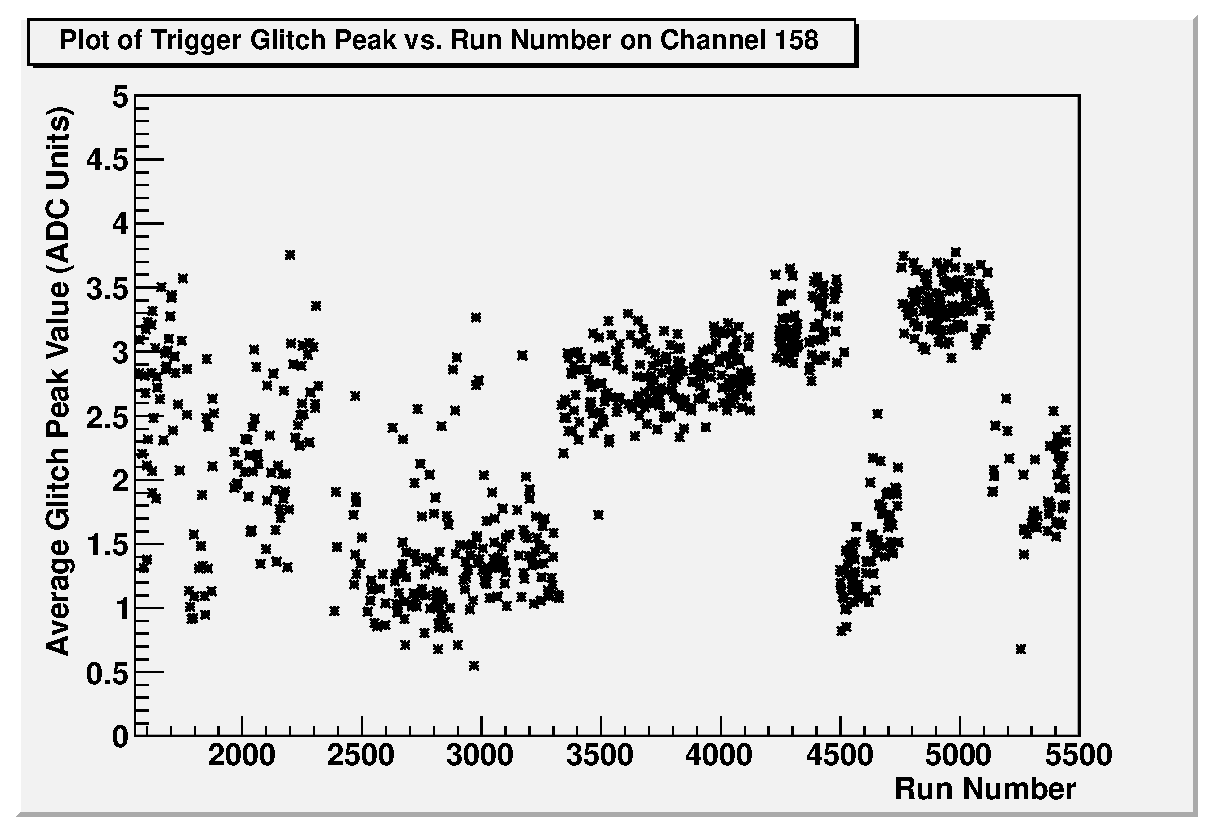
\includegraphics[keepaspectratio=true,width=\textwidth]{glitch_peak_vs_time_158.eps}
\end{center}
\renewcommand{\baselinestretch}{1}
\small\normalsize
\begin{quote}
\caption{The amplitude of the trigger-time ``glitch'' over time for channel 158.  Figure provided by Sam Homiller.}
\label{fig:GlitchPeakAmplitudeVsTime}
\end{quote}
\end{figure}
\renewcommand{\baselinestretch}{2}
\small\normalsize

stripping the glitch from noise traces.
using noise in monte carlo?
Studying the smoothness of the noise functions vs f (for truncated waveforms).
Check noise temperature dependence, other rapidly-varying environmental factors.
Resolution time-dependence can be used to check time windows; other approaches?  (KZ tests for consistency with flat.)

\renewcommand{\thechapter}{6}
\chapter{The Lightmap}
\label{ch:Lightmap}

EXO-200 uses a lightmap to characterize the expected scintillation pulse magnitudes from scintillation clusters with a known position and energy.  Chapter~\ref{ch:DenoisingResults} has shown that the lightmap is a critical input to the denoising algorithm.  In this chapter, we develop from a simpler type of lightmap used in prior analysis to a fully detailed individual-APD lightmap which characterizes scintillation pulse magnitudes on every channel as they depend on scintillation cluster position.  All of this is done in a time-dependent fashion, so the main result of this chapter will be, for each APD channel, a four-dimensional function of scintillation cluster position and time that yields the expected pulse magnitudes.  In section~\ref{sec:LightmapHistory} we describe the lightmap which existed prior to this work, its accomplishments, and its issues which made an upgrade necessary.  Section~\ref{sec:FourDimLightmapParent} will present details of the production of the lightmap from empirical data; deviations from that algorithm for the present analysis are presented in section~\ref{sec:LightmapImplementationDetails}.  Visualizations of the result are provided in section~\ref{sec:LightmapVisualization}.

\section{A History of EXO-200 Lightmaps}\label{sec:LightmapHistory}

The EXO-200 detector has roughly 450 APDs ganged into 74 data channels of five to seven APDs each. Three of the APD ganged channels were disabled due to noisy components before physics data collection began; a fourth channel was disabled in February 2012 due to increasing noise.  The APDs are set into the two endcaps of the cylindrical EXO-200 detector.  To improve light collection, teflon sheets cover the inside of the detector and reflect light back into the liquid xenon rather than allowing it to be absorbed by the vessel walls.

Scintillation is not collected uniformly by all APDs.  Given the same amount of energy deposited into the detector, APDs channels nearest to the deposited energy show significantly larger pulses than APD channels far from the deposit.   To accurately measure the true scintillation energy, it is critical to map out the response of the APDs as a function of deposit position $\vec{x}$.

Furthermore, the APDs and their front-end electronics show time-dependent changes. Gains drift in each APD channel at a variety rates, and stepwise changes occur when the electronics are changed or channels are disabled. This has happened on multiple occasions during the course of the experiment.  This means that, in addition to mapping the response of the APDs as a function of deposit position $\vec{x}$, we must also map it as a function of  time. We call this the lightmap.

Earlier lightmaps were derived from periodic source calibration campaigns collected over one or more days. The ``strong'' Thorium-228 source ($34.04$ kBq, or 0.9201 $\mu$Ci, on September 1, 2009~\cite{SourceCertificates}) was used, and an on-site expert would  position the source in a wide range of locations around the detector.  The $2615$-keV single-site gamma line of the Thallium-208 (a daughter product of Thorium-228) allows the pulse magnitude from a single-position mono-energetic deposit in the detector to be determined in offline analysis.

Even with such a significant quantity of source data, statistics are generally insufficient to fully characterize the lightmap with this method.  The source guide tube shown in figure~\ref{fig:CalibrationGuideTube} does not approach near to every region of the detector; as a result, some regions are difficult to illuminate with the 2615 keV gamma line.  Additionally, APD pulses on individual channels may be quite small for cluster positions which are not quite near to the APDs, compounding the problem of low statistics.  To simplify the problem, pulses on the waveforms of each endcap can be summed together (without gain corrections) such that the 70 or 71 active APD channels can be treated as merely two APD sum channels.  This effectively increases the size of the pulses and the signal-to-noise ratio of these waveforms. It also makes the spatial dependence of the response smoother, so that a coarser binning of the position coordinates is sufficient to characterize the response.  The resulting lightmap was characterized in~\cite{ThesisSteve} and used in~\cite{bb0nSearch2012,bb2nEXO2014} to perform a precision measurement of the rate of $\beta\beta 2\nu$ decay and a search for $\beta\beta 0\nu$ decay in $^{136}$Xe.

Although this lightmap produced significant improvements in the energy resolution achieved by the EXO detector,  it is an incomplete characterization of the APD response.  For example, for $\beta\beta0\nu$ studies we place a fiducial volume cut as close to the edges of the detector as possible, and in certain regions of the detector the scintillation pulse is highly concentrated on a small number of channels.  Summing together multiple channels is, in this case, a lossy form of compression of the data, and it is possible to extract a better energy measurement if it is avoided.

\begin{table}
\begin{center}
\begin{tabular}{|c|c|r|}
\hline Nominal Source Position & Deployment Position & Triggers \\
\hline P2\_nz & S2 & 6207613 \\
P4\_px & S5 & 85931937 \\
P2\_pz & S8 & 5395820 \\
P4\_py & S11 & 6775279 \\
P4\_ny & S17 & 5482649 \\
Other & Other & 1773128 \\ \hline
\end{tabular}
\end{center}
\caption{The total number of thorium triggers taken at each source position; data include only runs which were used to generate the lightmap.  Nominal source position follows a code where the number is 2 for anode runs and 4 for cathode runs; the second part of the code indicates the non-zero coordinate, eg. `px' means positive-x direction, `nz' means negative-z direction.  A diagram of the source tube is shown in figure~\ref{fig:CalibrationGuideTube}.}
\label{tab:TriggerStatsBySourcePos}
\end{table}

The present chapter addresses the challenges inherent with the formulation of an individual-APD lightmap.  We do this primarily by a significant increase in available statistics: whereas the older lightmap used thorium data from a specific calibration campaign lasting for only a few days, we combine all thorium data that has ever been collected by the EXO-200 detector between October 5, 2011 and June 24, 2013.  The total number of triggers included in this dataset are listed in table~\ref{tab:TriggerStatsBySourcePos}.  This vast extension of the available data raises the challenge that APD behavior is time-dependent, so pulse magnitudes may not be constant throughout the dataset; we account for this with a parametrization of the lightmap which permits us to simultaneously extract this time-dependent behavior and the position-dependent light yield that is independent of time.  The result is a complete characterization of light yield in EXO-200.

The denoising algorithm described in chapter~\ref{ch:DenoisingTheory} describes one analysis by which we can exploit knowledge of the behavior of individual APD channels; other analyses include reducing our scintillation thresholds by allowing us to search for pulses in subsets of the APDs rather than only in sums across entire endcaps.  Thus, characterizing the APD yield on individual APD-gang channels is a key component of denoising and may enable additional future studies which would benefit from individual APD channel information.  Section~\ref{sec:FourDimLightmapParent} describes the method used to extract an individual-APD lightmap.

\section{Four-Dimensional Lightmap}\label{sec:FourDimLightmapParent}

As described above, in constructing a channel-by-channel lightmap we face two conflicting needs: we must use as much data as possible to handle the rapid spatial variation and smaller pulses which are expected, but if too much data is included then we run the risk of combining data taken when an APD or the electronics had a different gain.  If we truly wish to use all available data, then we must simultaneously understand the full time-dependence of the gain.  In other words, rather than forming a small number of independently-measured three-dimensional lightmaps, we instead measure a four-dimensional lightmap $L(\vec{x},t)$.  Since we use Thorium-228 source data to generate the lightmap, we require that our lightmap should predict the magnitude of the pulses on each APD gang induced by a single-site deposit of energy $2615$ keV.  Figure~\ref{fig:SampleAPDTemplates} shows our definition of a unit-magnitude pulse.

This may at first seem infeasible.  After all, adding an extra time dimension to the arguments of the lightmap is equivalent to generating a new lightmap for every time bin, which is exactly the situation we wish to avoid.  But we can make a simplifying assumption that the lightmap is separable.  In a physical sense, we assume that:
\begin{enumerate}
\item From a given position $\vec{x}$, photons deposit on each APD channel at a constant rate.
\item Each APD channel amplifies and shapes its pulse with a gain which may vary in time, but does not depend on the point of origin of the photons.
\end{enumerate}
So, we demand that the lightmap have the much simpler form
\begin{equation} \label{eqn:SeparableLightmap}
L(\vec{x},t) = R(\vec{x})S(t)
\end{equation}

Although this is a reasonable approximation, there are details which are omited by this model.  Since the electric field and the reflectivity of detector surfaces are constant in time, assumption 1 is likely to be valid.

However, assumption 2 may not hold in certain cases. For example, each channel draws its pulse from multiple APDs, each of which has an independent time-varying gain.  Photons from a deposit may preferentially sample the gain from the closest APD within a channel, so deposits in different locations may track more closely the gain of the closest APD within a channel.  A study of the impact of this effect is a topic for future study. The analysis presented here will treat it as a small effect.

One simple scheme to find $R$ and $S$ iteratively is described in algorithm~\ref{alg:LightmapScheme}.  Step~\ref{algline:LightmapFormListOfHits} of that algorithm is to select $2615$-keV single-site events; it is understood that some compton-scattered events will inevitably leak into our selection window, but we use the best available energy measurements to minimize that likelihood. As analysis improvements continue to improve the energy resolution, the number of selected compton-scattered events will become smaller and the quality of the lightmap will improve.  The rest of the algorithm describes how we can efficiently converge on estimates of $R(\vec{x})$ and $S(t)$ through an iterative approach.  We do not prove that the algorithm is guaranteed to converge; however, in practice $S(t)$ is almost constant, resulting in fairly rapid convergence.

\begin{algorithm}
\caption{Generating a Lightmap}
\label{alg:LightmapScheme}
\algsetup{indent=2em} % Recommended by the package authors; the default is only for backward compatibility.
\begin{algorithmic}[1]
\STATE Tabulate, using the best energy measurement available, a list of single-site 2615-keV events from Thorium-228 source data. \label{algline:LightmapFormListOfHits}
\STATE Set $S(t) = 1$ for all APD channels.
\REPEAT
  \STATE For each APD channel, estimate $R(\vec{x}) = L(\vec{x},t)/S(t)$ from the set of events tabulated in line ~\ref{algline:LightmapFormListOfHits}.
  \STATE For each APD channel, estimate $S(t) = L(\vec{x},t)/R(\vec{x})$ from the set of events tabulated in line ~\ref{algline:LightmapFormListOfHits}.
\UNTIL convergence is reached.
\end{algorithmic}
\end{algorithm}


\section{Algorithm Details}

The previous section outlines a general algorithm for computing a four-dimensional channel-by-channel lightmap from source data.  In this section we specify the implementation choices which are made in the code currently in use by EXO-200.  In attempt to encourage future experimentation, alternative options will also be listed in some detail, along with some motivations for these alternatives.  Time has not permitted testing of all of these options, but it is hoped that they will be explored in the future.

\subsection{Event Selection}\label{sec:LightmapEventSelection}

The single-site Thorium-228 spectrum is well-peaked at 2615 keV, making it an excellent monoenergetic calibration line.  Our challenge is to select truly 2615-keV events as efficiently as possible, while simultaneously avoiding near-2615-keV events which may leak into the dataset.

This is inherently an iterative process.  The first lightmap is constructed from events selected based on an ionization-only spectrum because no useful position-corrected scintillation measurement yet exists. The resolution of the ionization-only spectrum is relatively poor, roughly $3.5\%$ (sigma) of the energy, as described in \cite{ThesisSteve}, and compromises are made to keep the Compton-shoulder leakage to acceptable levels.  \cite{ThesisSteve} required events to have ionization between $+0.33\sigma$ and $+3\sigma$ of the ionization peak.

Such a strongly asymmetric cut is chosen to avoid leakage from compton shoulder events.  However, because of the anticorrelation between scintillation and ionization, events whose ionization fluctuates high preferrentially selects events whose scintillation fluctuates low, introducing a bias in the pulse magnitude.  Additionally, the cut accepts less than $37\%$ of good events, which is a substantial loss of event statistics. This has a significant impact in certain low-statistics regions of the detector.

The current work benefits from this existing position-corrected scintillation measurement of \cite{ThesisSteve}, leading to a rotated energy spectrum with resolution of roughly $1.8\%$.  As a result, it is possible to accept more events while still keeping Compton shoulder leakage small.  We currently accept events within $2\sigma$ of the peak, with better than $95\%$ acceptance and only small leakage.  An additional benefit is that the improved energy resolution allows us to use a symmetric acceptance region, avoiding the implicit bias introduced from the earlier asymmetric cut window.

Preliminary investigations have been conducted to see the impact of using the denoised scintillation measurements which are the subject of this work in the event selection itself.  Presently the improvement in resolution (to $1.53\%$) has not demonstrated any significant improvement in the quality of the next iteration of the lightmap beyond what we can achieve with $1.8\%$ resolution. This is a topic of continuing study.

Beyond the cuts described above (single-site within an appropriate energy window), other basic cuts are applied to ensure only well-behaved scintillation pulses are selected (where we emphasize that all scintillation cuts are with reference to the old reconstruction scale, which was not normalized):
\begin{itemize}
\item Charge and light must individually lie within a reasonable range: charge must lie between 1 and 5000 uncalibrated keV, and light must lie between 1 and 15000 counts in the old scintillation reconstruction scale.
\item The charge-to-light ratio must not identify an event as an alpha decay: the light counts $L$ and charge counts $C$ must obey the relation $L < 3.405\cdot C + 2600.67$.
\item The scintillation time must be well-separated from any other scintillation clusters in same event frame: a scintillation cluster is only acceptable if no other scintillation clusters occur within 220 $\mu$s before or 180 $\mu$s after it.
\item All charge clusters which are assigned to this scintillation cluster must be assigned unambiguously: for each charge cluster assigned to this scintillation cluster, there can be no other scintillation cluster occurring within 140 $\mu$s before or 5 $\mu$s after it.
\item All three position coordinates of the charge deposit must be reconstructed.  (No fiducial cut is placed, since that would restrict the volume where the lightmap is specified.)
\end{itemize}
Many of these cuts are probably unnecessary. As the energy resolution has improved, the chances of Compton-shoulder contamination have decreased. Note that our $\beta\beta 0\nu$ decay search analysis only accepts events with a single scintillation cluster, a requirement which would carry a high cost in lost statistics for determination of the lightmap.  (Strong thorium runs ($34.04$ kBq, or 0.9201 $\mu$Ci, on September 1, 2009~\cite{SourceCertificates}) produce a significant rate of events with multiple scintillation clusters.  These statistics are quite valuable, particularly because they are the primary source of events in some poorly illuminated regions of the detector.)  

\subsection{Function Parametrization} \label{sec:LightmapFunctionParametrization}

Because we are attempting to empirically measure the functions $R(\vec{x})$ and $S(t)$ from a finite dataset, we must specify some more limited form for them to take.  All current approaches to describing $R(\vec{x})$ first bin the detector volume into three-dimensional voxels, and then define $R(\vec{x})$ to interpolate linearly between known values at the center of the voxels.  The size of these voxels must be chosen with some care; if they are too small, then low per-voxel statistics cause the statistical errors on the pulse magnitude to dominate, whereas if the voxels are too large then the spatial variation of the lightmap is not fully captured.

In the current lightmap, the detector is binned into 1 cm$^3$ voxels; the detector is easily contained within a box with sides 40 cm long, leading to $64,000$ voxels (of which roughly $20\%$ lie outside of the detector and will be empty).  The choice of voxel size was made based on the size of an individual APD, which is roughly 2.5 cm in diameter. Very near the anode we would like for the size of a voxel to be much smaller than 2.5 cm.  When 1 cm$^3$ voxels are used, much of the detector has sufficient statistics per voxel; however, there are some regions of the detector with fewer than ten hits per voxel, indicating that $R(\vec{x})$ may have quite significant statistical error in these regions.

It is possible to justify a choice of larger voxels.  The APDs lie at $\pm 204$ mm from the cathode, which means that there is more than 2 cm between our fiducial volume and the APDs.  At this distance, the dependence of the lightmap on $x$ and $y$ is expected to be much slower than at the APD plane, indicating that perhaps 2 cm binning in $x$ and $y$ may be sufficient.  Additionally, $z$-dependence of the lightmap is expected to be fairly smooth throughout the detector. Since we interpolate linearly between voxels, it may be possible to use a $z$-binning much coarser than 1 cm.  This is a topic for future investigation.

It is also worth mentioning that alternative voxel geometries have been tried in the past.  The older APD-plane lightmap~\cite{ThesisSteve} used a cylindrical-coordinate binning. Binning in $r$ was selected to make the bin volumes roughly constant along the $r$ axis, binning in the angular coordinate was uniform, and binning in $z$ was chosen to be coarser near the anodes and finer near the cathode to reflect faster variation there.  In all cases the binning was coarser than with the current cubic voxels being used. Our finer binning is made possible by the larger quantity of available statistics from using the full dataset, and is justified by the potential for the yield on a single APD gang to vary more rapidly than the yield averaged across an entire APD plane.

It is well-known~\cite{MultivariateDensityScott} that when it is necessary to estimate a multivariate function from limited statistics, a choice of binning can have a significant impact on the result.  It is preferable to use an unbinned technique such as kernel regression.  In particular, our data density is highly non-uniform, and it should be possible to measure the lightmap with high fidelity in regions of high statistics, while smoothly transitioning to a coarser interpolation in regions of low statistics to minimize the impact of uncertainty from individual hits.  State-of-the-art solutions to this problem would rely on locally adaptive kernel regression; see~\cite{MultivariateDensityScott} for a detailed explanation of the related issues in non-parametric multivariate regression.  Attempting to use a locally adaptive kernel regression for $R(\vec{x})$ should be considered a highly appealing extension to the algorithm described here for generating a lightmap.

The parametrization of $S(t)$ presents a very different set of choices.  Thorium data is taken in bursts, with the time between mostly filled by low-background runtime.  When we choose to treat $S(t)$ as a smoothly varying function, it becomes critical to interpolate properly -- after all, the low-background runtime is the critical part of the experiment.  (If we only produce a lightmap accurate during source calibration runtime, we will measure an energy resolution from source data which is not borne out in the low-background data, so we should in fact be able to give some guarantee that $S(t)$ is almost as accurate during the low-background runtime as during the source runtime.)  Fortunately, it is generally true that the time variation of the APD response is quite slow; exceptions are generally due to changes in the electronics which occur at well-specified times.

Currently each source run is treated as a burst of data taken at the midpoint of the run, and $S(t)$ is measured at that point only from the data of that run; then $S(t)$ is linearly interpolated between those points.  In principle it is possible that between two source runs an electronics change may have been performed, which would mean that a better interpolation would be to assume $S(t)$ is flat except for a step at the time of the electronics change; in practice, though, EXO-200 has generally taken a source run immediately before and after an electronics change, so no high-value data is taken during that interval and this detail can be ignored.

Another concern with this method is the treatment of short source runs.  If a run is too short, then the measurement of $S(t)$ coming from that run may have significant errors.  We currently mitigate this issue by entirely throwing out all data from runs with fewer than $100$ usable events.  We justify this approach by claiming that even though those events might in principle have contributed some useful information on $R(\vec{x})$, without a good measurement of the relevant $S(t)$ it is impossible to use that data.

In the future, it would be useful if instead we performed smoothed interpolations between electronics changes.  This could be done in the same style as EXO's lifetime corrections, using polynomial fits, where the degree of the polynomial could be determined by eye.  A candidate set of time intervals when $S(t)$ might be treated as constant could be the same as the set of constant noise windows described in chapter~\ref{ch:NoiseMeasurements}.  It would be possible to check whether this time binning is fine enough by looking at the thorium scintillation peak position versus time in denoised data -- if it appears to drift in time within a window where $S(t)$ is treated as constant, then it is likely that $S(t)$ needs to be binned more finely.

Alternatively, often there is a long string of consecutive source runs which should be combined into one higher-statistics dataset.  This process must be done by hand, and has not been performed for the current analysis, but it could benefit the accuracy of the $S(t)$ function and also recover some statistics in cases where the individual runs might be too short for inclusion in the lightmap dataset.

The choice of binning or parametrization for $R(\vec{x})$ and $S(t)$ can have a profound impact on the accuracy of the lightmap, and the current analysis has only skimmed the surface of the various options.  It is hoped that further work on the lightmap will include significant investigation in these topics.

\subsection{Convergence and Error Estimation}

Our treatment of the convergence of algorithm~\ref{alg:LightmapScheme} and the resulting statistical errors in $L(\vec{x}, t)$ is rudimentary.  Cronvergence is checked not by analysis of the lightmap itself, but by verifying that the energy resolution from denoising is not improved by further iterations through algorithm~\ref{alg:LightmapScheme}.  Lightmap errors do not directly enter into the calculations of denoising (which treats the lightmap as perfectly known), so they are not estimated at all in the current analysis.

As a proxy for estimation of the statistical errors in the lightmap, we instead study the number of hits observed in each position voxel of the detector (see section ~\ref{sec:LightmapVisualization}), and presume that the most significant source of error comes from low-statistics regions of the detector.  This information can motivate future data-taking campaigns to probe the light response in those regions of the detector and reduce these uncertainties.  However, no explicit estimation of the lightmap uncertainty has been attempted.

One difficulty with estimating the errors in the lightmap function $L(\vec{x},t)$ comes from the correlation between errors in $R(\vec{x})$ and $S(t)$.  If one of those two components were known perfectly, then we could treat the fit uncertainties of each hit as independent errors, and propagate those errors into an uncertainty for each voxel of $R(\vec{x})$ (if $S(t)$ is assumed to be perfectly known) or $S(t)$ (if $R(\vec{x})$ is assumed to be perfectly known).  But on the contrary, all of the measurements of $R(\vec{x})$ are correlated with all of the measurements of $S(t)$, meaning that even the errors of different voxels of $R(\vec{x})$ or different times in $S(t)$ are correlated with each other.  Fully characterizing these errors would require a significant effort and computation.

Although a full estimate of lightmap errors with correlations would probably be computationally quite intensive to produce, it might be possible to estimate the independent errors of each voxel of the position lightmap $R(\vec{x})$ or each independent run making up $S(t)$ by treating the other function as perfectly known, as described above.  This would generally produce an underestimate of the uncertainty in each, but the estimate might still give some benefit.

To produce a more accurate estimate of errors, it would probably be necessary to do a simultaneous fit by varying both $R(\vec{x})$ and $S(t)$ together.  In the current scheme, $R(\vec{x})$ contains far more complexity than $S(t)$ with roughly $50,000$ non-empty voxels, so for each APD gang we would need to simultaneously vary roughly $50,000$ parameters to obtain the optimal lightmap.  It is exactly this time-intensive process which was avoided by choosing the iterative approach for measuring the lightmap; however, it would only need to be performed occasionally when deriving a new lightmap, so it is not infeasible to imagine attempting this project.  The prospect of feeding in a high-quality guess obtained from the iterative method presents an additional significant time-saver.  This method would not fully account for the correlations between errors of the different voxels of $R(\vec{x})$ or runs in $S(t)$, but it would come closer than the naive method described earlier.

However, it is also possible that identifying the error of each voxel or run is heading down the wrong path.  As described earlier, it is likely that the optimal (lowest-error) method for estimating the lightmap will be an unbinned method such as a locally-adaptive kernel regression method.  Error estimation in kernel regression presents significant additional challenges compared to errors from binned parametrizations.  At present, I am not aware of any simple scheme to manage this difficulty, meaning that there may be a paradoxical tradeoff that using the best method for minimizing lightmap errors simultaneously makes those errors infeasible to estimate.

Note that under the iterative method, the most naive method for estimating errors is not valid.  It might appear that when $S(t)$ is initialized to a constant value of $1$, we could also assign to it some constant error.  Then when we compute $R(\vec{x})$, we could propagate independent errors from the fit uncertainties of pulses and from $S(t)$; and when we compute $S(t)$ we could propagate independent errors from the fit uncertainties and from $R(\vec{x})$; and so forth.  However, such a scheme provides no compensating feedback mechanism to force the iterated errors to a reasonable or accurate value, so there is no reason to believe the errors from such a system (if, that is, they converge at all).  This difficulty may underscore the fundamental challenge associated with measuring the lightmap errors within our scheme -- iterative methods are well-suited to solving a system, but when correlated errors are mistreated as uncorrelated an iterative method can easily magnify the impact of that mistreatment.

On the topic of convergence, it has been mentioned already that by starting with a generally accurate initial guess for $S(t)$ as constant, the iterative solution method tends to converge rapidly.  As a result, and because iterations take only a few hours to perform on a single machine, we currently perform three iterations and claim that convergence is approximately reached.  Ideally, we would require that none of the position voxels or runs change value within an iteration by more than some fraction of their estimated errors; but in the absence of estimated errors, this is of course impossible.

It would be possible, in a conservative approach, to require each value to converge to some small fraction of an ADC unit, ensuring that the convergence is better than our ability to measure pulses.  Such a requirement might force us to compute more iterations than are truly warranted by our lightmap errors, but given the reasonable speed of each iteration, such a method still might not be unreasonable.

\section{Implementation for this Analysis}\label{sec:LightmapImplementationDetails}

The physics analysis which will be described in this paper includes data from EXO runs $2464$ to $5597$, which were taken between October 5, 2011 and September 1, 2013.  However, at the time when the initial denoising processing was begun, the tentative range of runs to be used only extended up to $5367$ on June 24, 2013.  As a result, calibrated data at that point was only available up to June 24, 2013, and the lightmap had only been generated using the same set of thorium source data.

When the run range for the present analysis was extended, a significant portion of the dataset had already been denoised with the lightmap based only on data extending to June 24, 2013.  Although the possibility of creating a new lightmap was considered, this would have required a re-analysis and re-verification of the existing denoised dataset.  As a result, the existing lightmap continued to be used.  The functions $S(t)$, which had only been directly measured up to June 24, 2013, were assumed to remain constant between June 24 and September 1, 2013; no known changes to the APDs occurred during this time, nor did any known environmental factors change, so this assumption was considered acceptable.  Future lightmaps of course will make use of a more complete dataset rather than relying on extrapolation.

Furthermore, one bug was discovered in the lightmap which was used for denoising.  A set of Radium-226 source data was taken before the corresponding identifier could be set in data files, and as a result they were provisionally labeled as thorium runs.  These runs were mistakenly incorporated into the generated lightmap, and events from the $2204$-keV gamma line of the Bismuth-214 daughter product of Radium-226 were selected and handled as though they were legitimate $2615$-keV events.

It was possible to partially remedy this after the fact: since currently there is a one-to-one relationship between individual source runs and their corresponding points in the functions $S(t)$, it was possible to artificially erase the data points of $S(t)$ originating from Radium runs.  It is not so easy to remove the impact they may have had on $R(\vec{x})$.  However, the Radium runs were taken at a location which is extremely well-populated by thorium data throughout the life of the detector; since the quantity of Radium data is small by comparison, the effect on $R(\vec{x})$ is presumed to be quite small.  Subsequent studies using a correctly-generated lightmap on small subsets of data indicate that the effect is indeed negligible, as expected.

\section{Visualization} \label{sec:LightmapVisualization}

\begin{figure}
\begin{center}
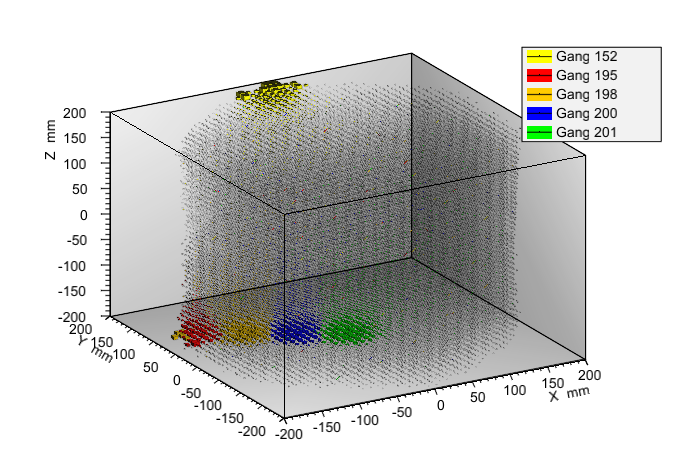
\includegraphics[keepaspectratio=true,width=\textwidth]{Lightmap_viz.png}
\end{center}
\renewcommand{\baselinestretch}{1}
\small\normalsize
\begin{quote}
\caption{Lightmap position-dependence $R(\vec{x})$ for selected APD gangs.}
\label{fig:Lightmap3DPlot_unzoomed}
\end{quote}
\end{figure}
\renewcommand{\baselinestretch}{2}
\small\normalsize

\begin{figure}
\begin{center}
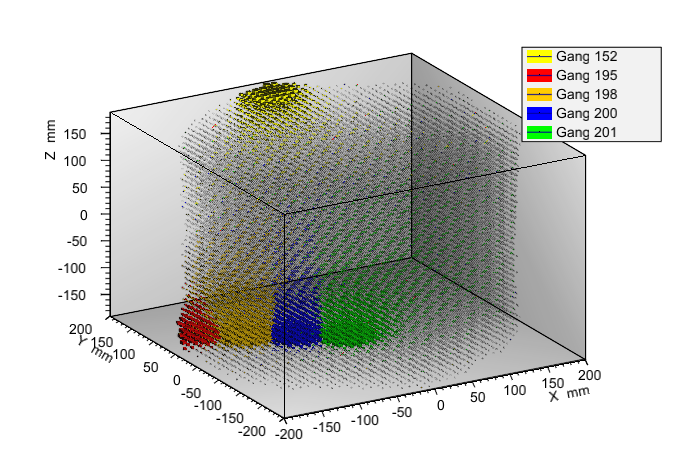
\includegraphics[keepaspectratio=true,width=\textwidth]{Lightmap_viz_zoom.png}
\end{center}
\renewcommand{\baselinestretch}{1}
\small\normalsize
\begin{quote}
\caption{Lightmap position-dependence $R(\vec{x})$ for selected APD gangs.  Here extreme anode positions are omitted to permit better contrast for the lightmap in the fiducial volume.}
\label{fig:Lightmap3DPlot_zoomed}
\end{quote}
\end{figure}
\renewcommand{\baselinestretch}{2}
\small\normalsize

\begin{figure}
\begin{center}
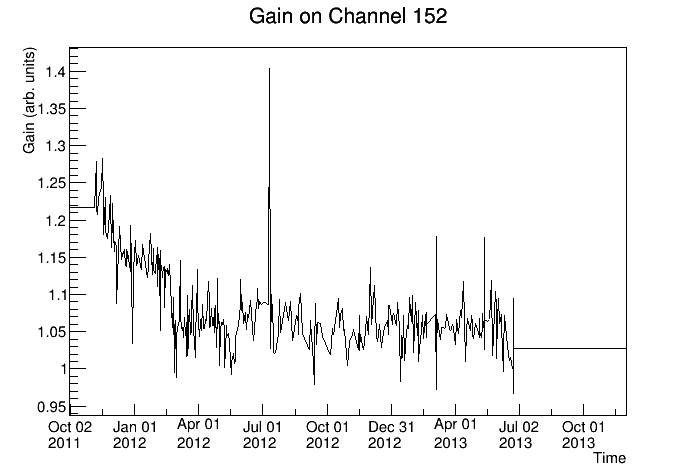
\includegraphics[keepaspectratio=true,width=\textwidth]{gainfunc_152.png}
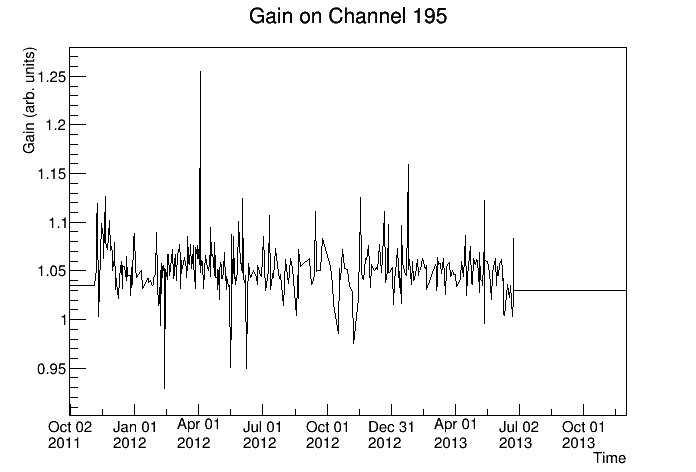
\includegraphics[keepaspectratio=true,width=\textwidth]{gainfunc_195.png}
\end{center}
\renewcommand{\baselinestretch}{1}
\small\normalsize
\begin{quote}
\caption{Functions $S(t)$ for selected channels.}
\label{fig:LightmapGainFunc1}
\end{quote}
\end{figure}
\renewcommand{\baselinestretch}{2}
\small\normalsize

\begin{figure}
\begin{center}
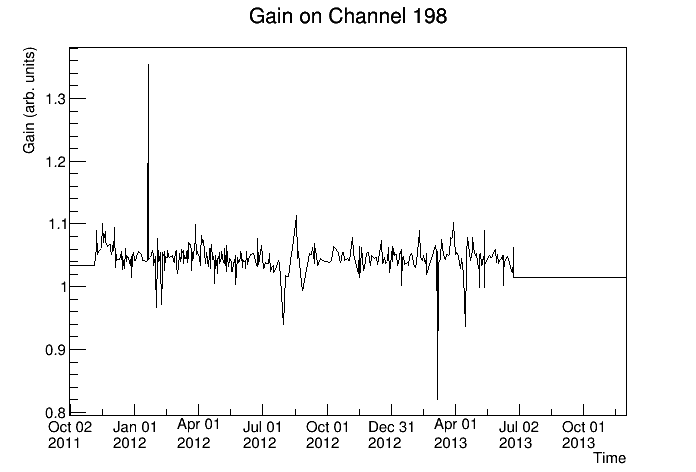
\includegraphics[keepaspectratio=true,width=\textwidth]{gainfunc_198.png}
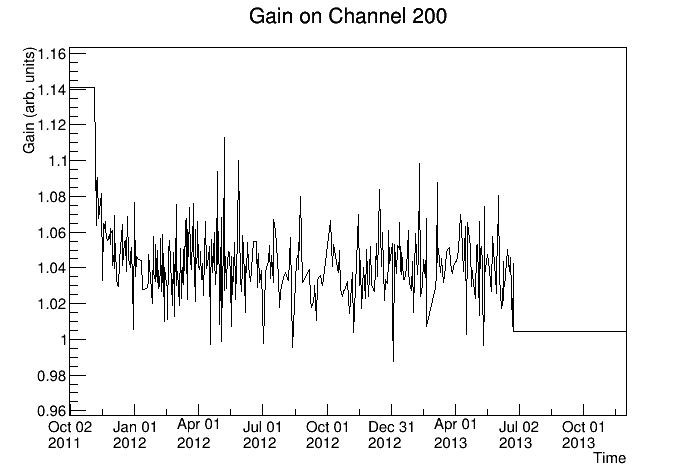
\includegraphics[keepaspectratio=true,width=\textwidth]{gainfunc_200.png}
\end{center}
\renewcommand{\baselinestretch}{1}
\small\normalsize
\begin{quote}
\caption{Functions $S(t)$ for selected channels.}
\label{fig:LightmapGainFunc2}
\end{quote}
\end{figure}
\renewcommand{\baselinestretch}{2}
\small\normalsize

\begin{figure}
\begin{center}
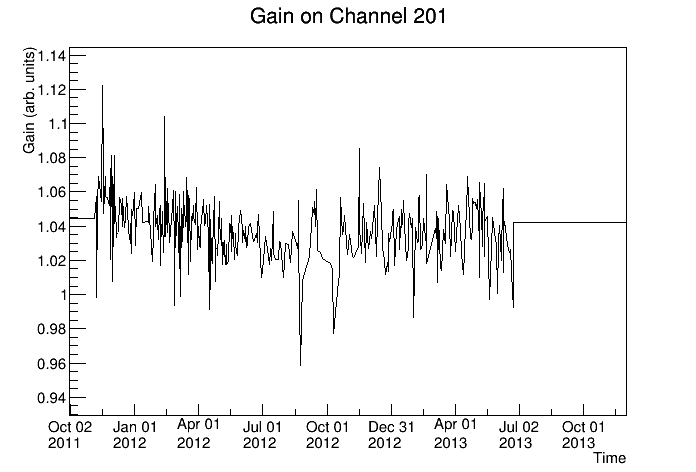
\includegraphics[keepaspectratio=true,width=\textwidth]{gainfunc_201.png}
\end{center}
\renewcommand{\baselinestretch}{1}
\small\normalsize
\begin{quote}
\caption{Functions $S(t)$ for selected channels.}
\label{fig:LightmapGainFunc3}
\end{quote}
\end{figure}
\renewcommand{\baselinestretch}{2}
\small\normalsize

Although it is not strictly necessary to be able to visually inspect the lightmap for it to be useful, nevertheless it is reassuring to see that the lightmap is qualitatively similar to intuitive expectations of how light should propagate through the detector.  We have chosen to store the position-dependent $R(\vec{x})$ for each APD gang as a set of ROOT TH3D objects, and fortunately ROOT provides a number of excellent plotting features suitable for a three-dimensional dataset.  In figure~\ref{fig:Lightmap3DPlot_unzoomed}, it is possible to view the values of $R(\vec{x})$ for a sample of gangs on top of each other.  Larger boxes and denser color indicates a higher yield on the APD gang in question, and it is immediately apparent that events near the anodes produce light which is highly concentrated on a single APD gang.

Figure~\ref{fig:Lightmap3DPlot_unzoomed} shows the highest yield on the very boundary of the detector, well outside of our fiducial volume; to permit us to more easily view contrast inside of the detector, figure~\ref{fig:Lightmap3DPlot_zoomed} shows the same map while omitting the most extreme bin near either anode.  Viewing this map, we can see more interesting characteristics of the lightmap:
\begin{itemize}
\item Events near the anodes show a high pulse concentration on the one gang nearest to their position; however, even deep into the detector near the cathode it is still possible to see the higher concentration of pulse magnitude on the gang directly aligned with the event.
\item We can also see, from gang 201 (green) in this visualization, that events can produce significant pulse magnitudes on APD gangs which which they are not directly aligned (in the Z direction); yield on gang 201 can be seen to decrease smoothly in all directions.
\item APD gangs in the corners of the detector, such as gang 195 (red), are not effective at measuring light from events which are far away; even directly above gang 195, it is clear that gang 198 is more effective at collecting light farther away than about five to ten centimeters.  This can be attributed to the reflection of photons by teflon, which may enhance the light yield on gangs which are not hidden in corners.
\end{itemize}

Figures~\ref{fig:LightmapGainFunc1}, \ref{fig:LightmapGainFunc2}, and~\ref{fig:LightmapGainFunc3} show the functions $S(t)$ for the same sample of gangs.  The vertical scale can be treated as having arbitrary units; we note that all of these functions lie roughly around $1$, which is attributed to the initial placement of $S(t) = 1$ in algorithm~\ref{alg:LightmapScheme}.  We draw the following primary observations from these plots:
\begin{itemize}
\item Many of the gangs show their values of $S(t)$ decreasing rapidly up to around February 2012; some of the gangs also show a sharp decrease in value at that point.  The decrease in gain corresponds with observations which were made at the time, leading to a decision to replace electronics on some APD channels on February 23, 2012.  Thus, we do see ``real" features from these plots.
\item The functions $S(t)$ are otherwise dominated by jitter between points, indicating that we do not collect enough statistics from each run to sufficiently constrain $S(t)$.  This is taken as the strongest evidence that we should use a coarser time binning for $S(t)$, as described in section~\ref{sec:LightmapFunctionParametrization}.  Preliminary work has been performed to do this with more recent lightmaps, but no studies have evaluated the impact on energy resolution.
\item Individual points on these functions may spike by as much as $40\%$.  These points have been investigated, and their cause is not understood.  These jumps, along with the overall jitter, will certainly be reduced by the use of a coarser time binning.
\end{itemize}

\section{Summary}

In this chapter we have described the generation of an individual-APD lightmap which characterizes the expected pulse magnitude on each APD channel as a function of scintillation origin, calendar time, and the quantity of energy.  The two key steps to this process are the use of the full dataset for extra statistics and the assumption that the lightmap is separable between position and time coordinates, as shown in equation~\ref{eqn:SeparableLightmap}.  Previous lightmaps could only characterize the light yield on large sums of waveforms; by providing a full lightmap for every channel, we enable the denoising algorithm of chapter~\ref{ch:DenoisingTheory} to make use of channel-by-channel pulse and noise information, so this lightmap is a key component of denoising and the improvement in resolution presented in section~\ref{sec:ResultComparison}.


\renewcommand{\thechapter}{6}
\chapter{EXO-200 Analysis and Results from Denoising}
\label{ch:DenoisingResults}

Data analyzed for the present work extends from \textcolor{red}{DATE to DATE}.  In this chapter, sections~\ref{sec:ResultSimulation}-\ref{sec:ResultFitting} describe the basic elements of the EXO-200 analysis.  Section~\ref{sec:ResultResults} will present the results from this set of data.  In section~\ref{sec:ResultComparison} we compare the results obtained using the denoising scheme of chapter~\ref{ch:DenoisingTheory} to the results which would have been obtained without that algorithm applied, and demonstrate that denoising has contributed to the strength of our physics reach.

\section{Simulation}\label{sec:ResultSimulation}

Here we will describe the simulation of radioactive sources in the EXO-200 detector.  We begin by describing the framework for simulating the deposition of energy from primary decay particles into the liquid xenon and surrounding materials.  From there, we continue to describe the simplified electric field model which permits us to model the drift of ionization towards the anode wires.

\subsection{Simulation of Particles using GEANT}

To simulate the deposition of energy from primary decay particles, version 4.9.3p02 of the GEANT software package is used.~\cite{Agostinelli2003250}\cite{1610988}  This package includes a database containing attenuation properties of many common materials as well as detailed decay modes for most radioactive isotopes.  Angular correlations between gammas are not modeled with this version of the software, but that is expected to be a minor detail and will be corrected by upgrading to a newer version of GEANT in the future.  Forbidden beta decays are generated with an incorrect beta spectrum in the default GEANT software; this is addressed by the EXO collaboration by using our own beta spectra where appropriate.

\begin{figure}
\begin{center}
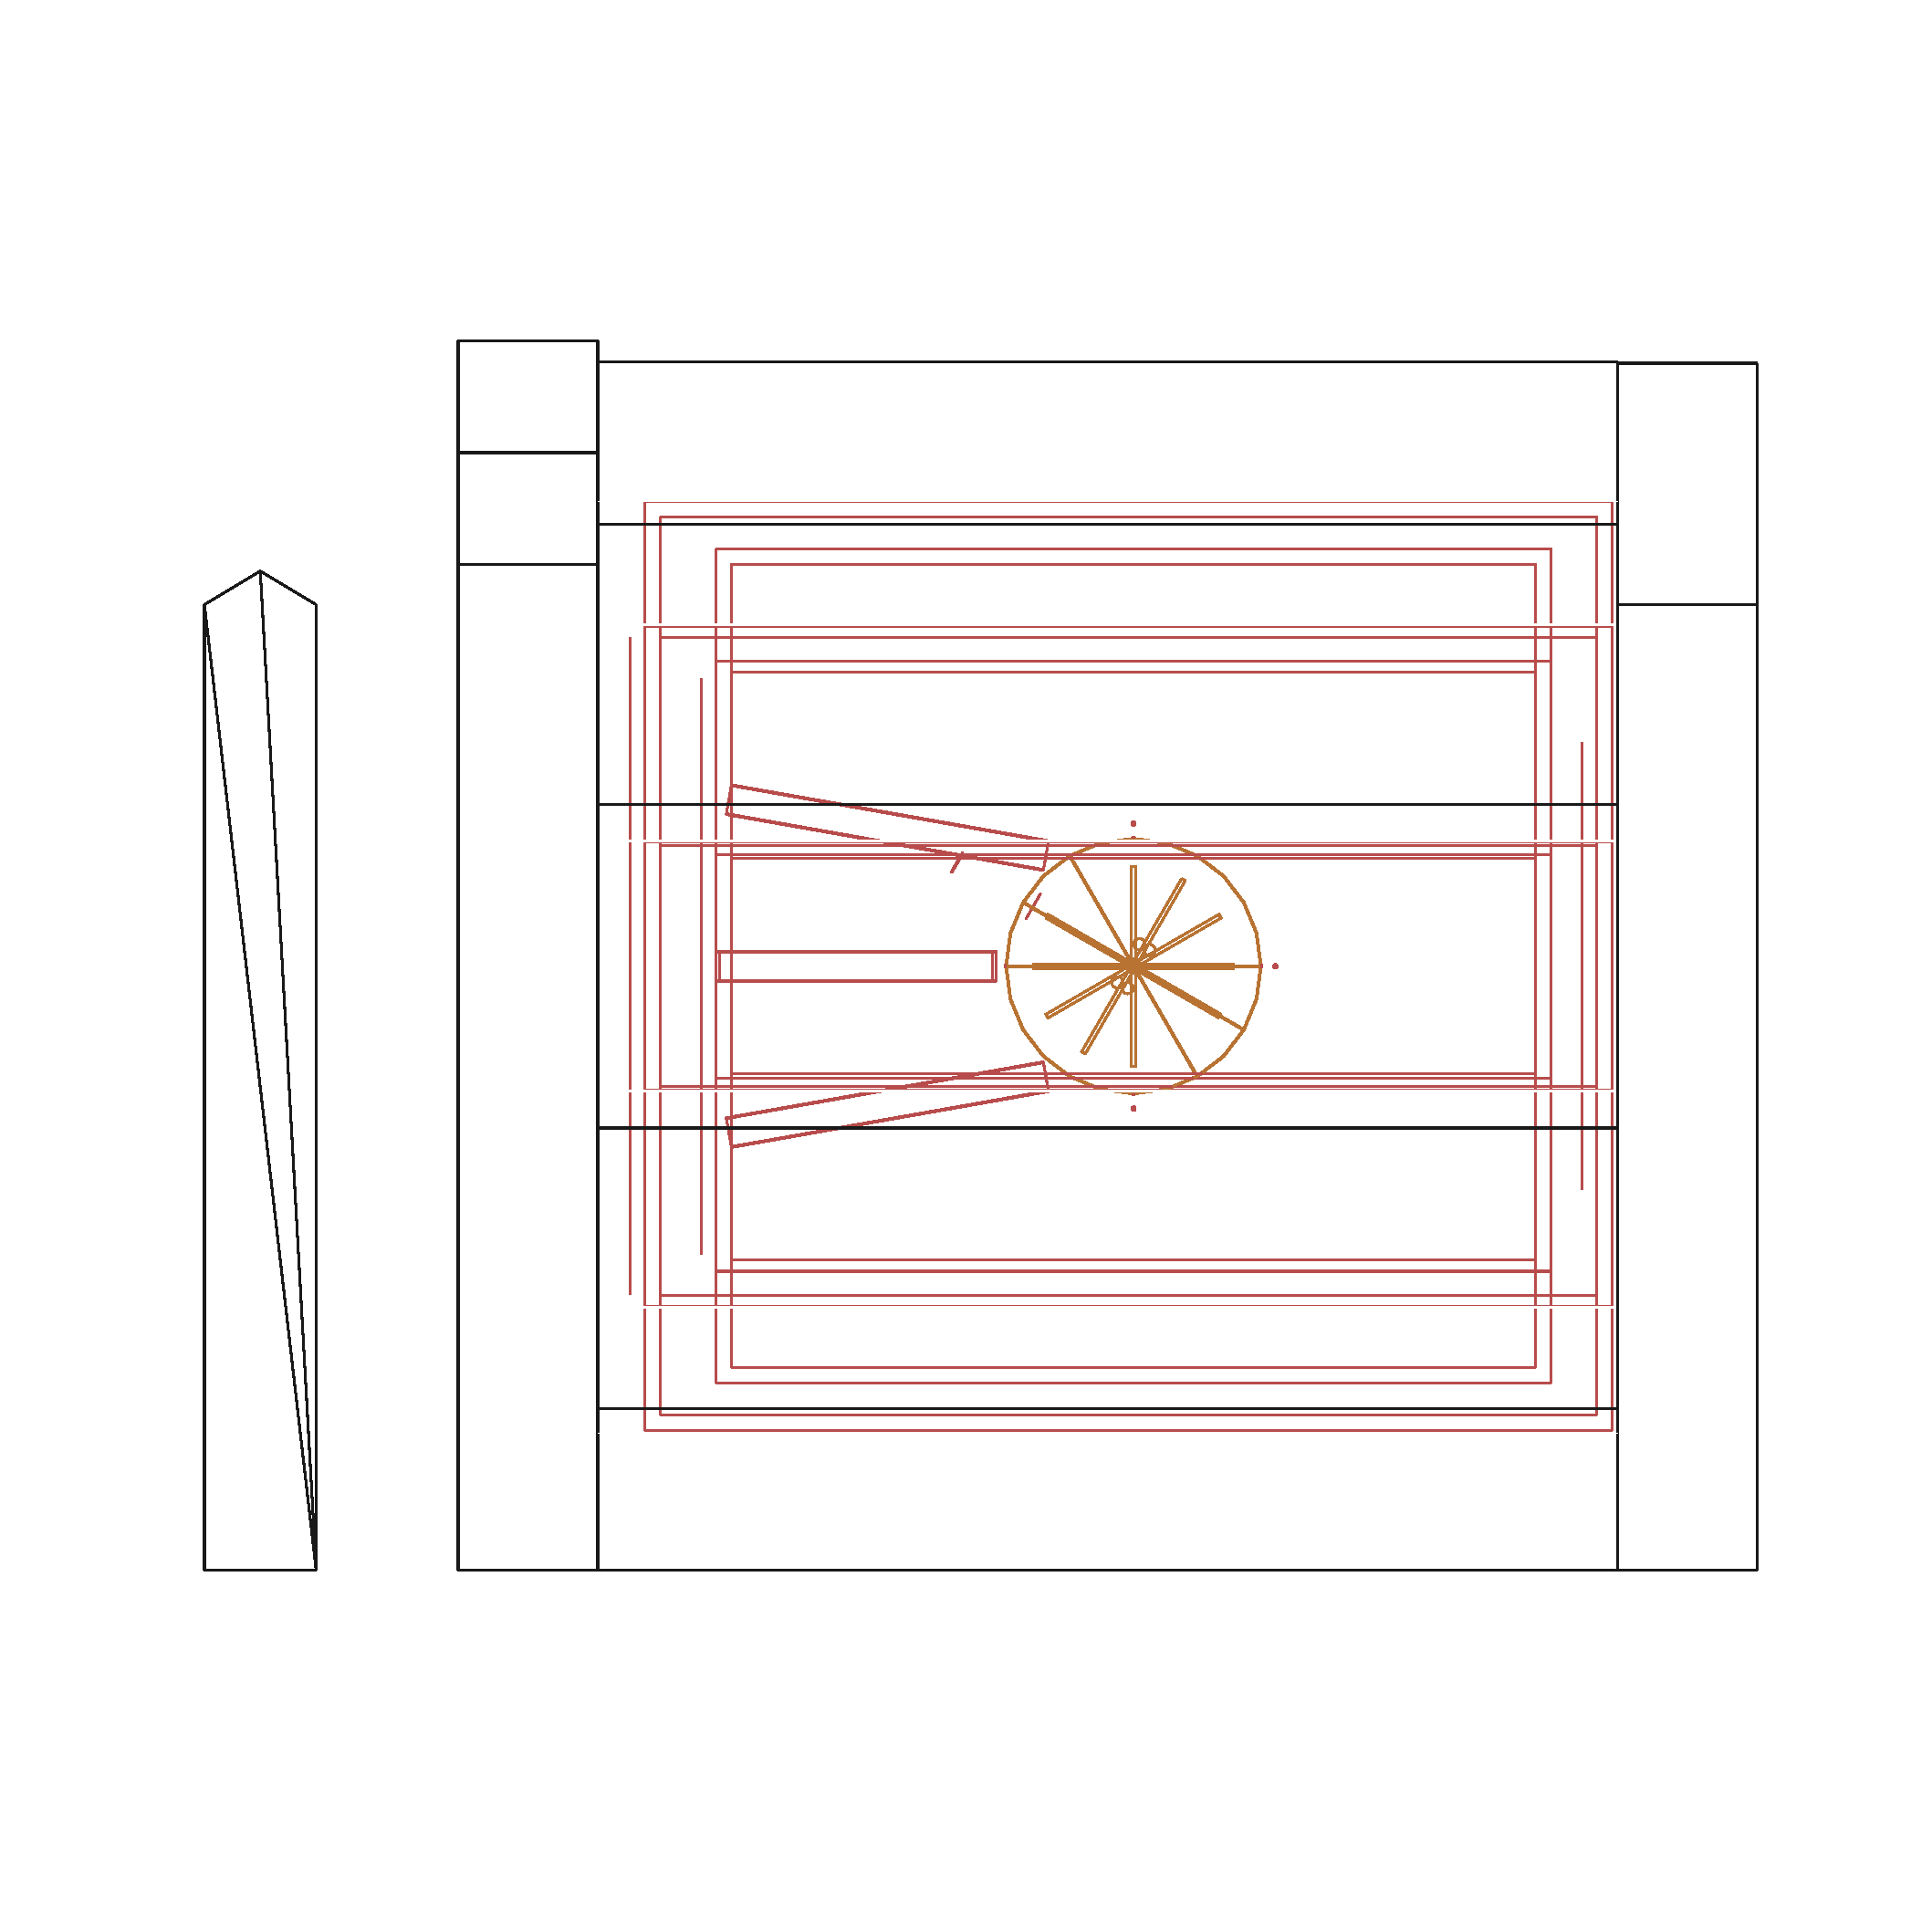
\includegraphics[keepaspectratio=true,width=\textwidth]{OGL_wireframe.eps}
\end{center}
\renewcommand{\baselinestretch}{1}
\small\normalsize
\begin{quote}
\caption{The GEANT simulation includes large-scale features of the EXO-200 detector, including the outer and inner lead wall (black), outer and inner cryostat and TPC legs (red), and the TPC itself (brown).  Components are assembled from simple geometrical shapes, and distant objects are only described coarsely.~\cite{MCDocumentRun2a}}
\label{fig:OGL_wireframevis}
\end{quote}
\end{figure}
\renewcommand{\baselinestretch}{2}
\small\normalsize

\begin{figure}
\begin{center}
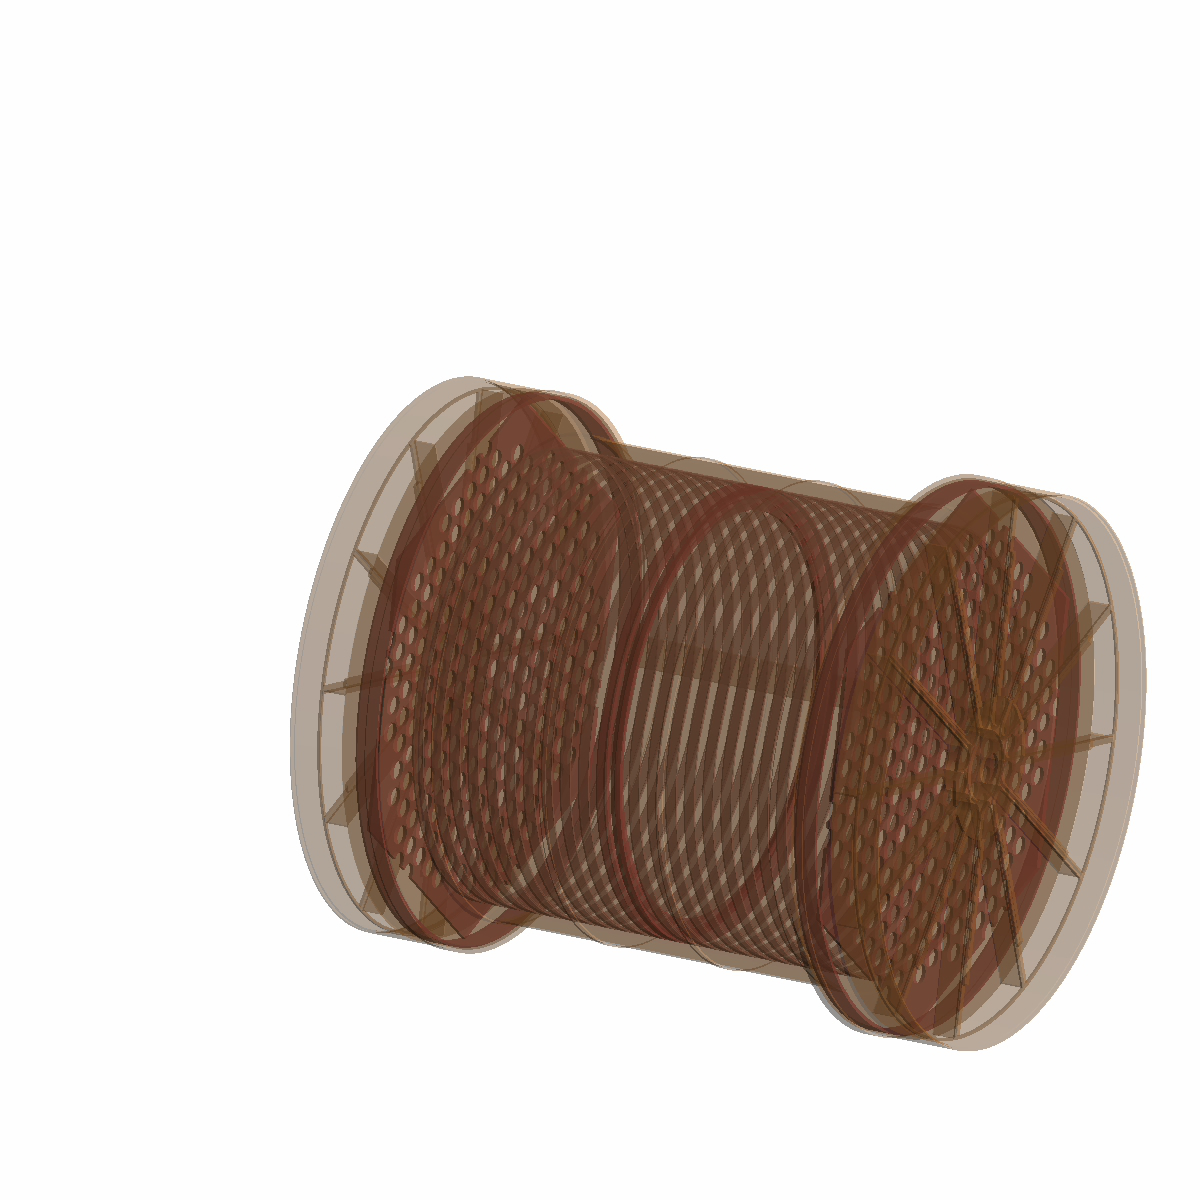
\includegraphics[keepaspectratio=true,width=\textwidth]{TPC_Cu_RayTracer.png}
\end{center}
\renewcommand{\baselinestretch}{1}
\small\normalsize
\begin{quote}
\caption{Detector components which are close to the liquid xenon are simulated in GEANT with far greater accuracy than distant objects, to reduce computational time.~\cite{MCDocumentRun2a}}
\label{fig:RayTracer_TPConly}
\end{quote}
\end{figure}
\renewcommand{\baselinestretch}{2}
\small\normalsize

A model of the EXO-200 detector is simulated in GEANT with a collection of simple geometric volumes, which can be composed to form more complicated structures.  Simulation speed decreases as more volumes are generated, and we expect that it is unimportant to simulate details much smaller than the distance between the detail and the liquid xenon.  We attempt to find a balance between accurate modeling of detailed features and simplification of distant features.  In figure~\ref{fig:OGL_wireframevis} we see the full geometry described in GEANT, where distant objects are constructed from a small number of geometric pieces.  Figure~\ref{fig:RayTracer_TPConly} shows how the TPC is described in GEANT, and we can see the level of detail is much greater.

To simulate particles, GEANT uses a Monte Carlo method.  It models particles as taking a sequence of steps, where each step is randomly generated; the probability distribution of each choice of step is determined by known properties of the particle, the energy of the particle, and the properties of the attenuating material.  The precise set of physical processes which determine the probability distribution is user-selected, and in EXO-200 has been chosen to include all processes which are significant within our energy range of 10 keV to 10 MeV.~\cite{MCDocumentRun2a}

Only energy which deposits in the liquid xenon is observable.  When primary decays are simulated far from the detector, it may be that most of those simulated events deposit no energy in the liquid xenon and are not observable; the simulation must continue running until a sufficient number of simulated events deposit energy in the liquid xenon.  This means that sources which are farther from the liquid xenon require significantly more computational time to accumulate a usable number of statistics.  We find that sources outside of the HFE are subject to $4.5$ attenuation lengths before reaching the liquid xenon, and events reaching the liquid xenon from the inner cryostat can only be simulated at $0.01$ Hz/core by this approach.~\cite{MCDocumentRun2a}

To improve this rate, importance sampling is employed for distant sources.  This approach consists of the following techniques to magnify statistics from a fixed simulation time:
\begin{itemize}
\item Low-energy beta and alpha particles outside of the TPC may be ``killed'', or prematurely eliminated from the simulation based on an expectation that they will not deliver any energy to the liquid xenon.
\item The detector is surrounded by importance sampling ``boundaries'': when a particle passes into a boundary it may be cloned (with a user-selected probability), where the rate of cloning is tracked by a corresponding decrease in particle ``weight.''
\item To avoid biasing the spectrum, it is also necessary to kill particles which pass out of a boundary with the same probability, and increase their weight accordingly.
\end{itemize}
This approach has the effect of using GEANT to simulate the properties of particles reaching the outermost boundary; then draw samples from that distribution and simulate the properties of particles reaching the next boundary; and so forth, amplifying the impact of statistics at each stage.  Further details on this approach can be found in~\cite{Dressel:642987}; it has the effect of increasing simulation speeds from the inner cryostat from $0.01$ Hz/core to a few Hz/core, and makes simulations of backgrounds from outside the lead wall feasible.~\cite{MCDocumentRun2a}

\begin{figure}
\begin{center}
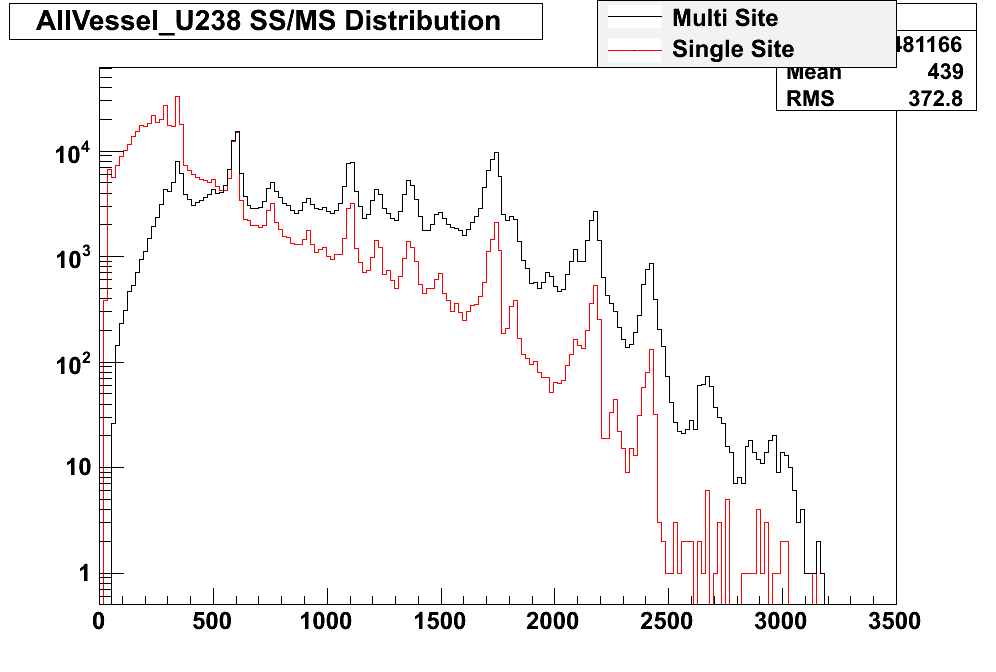
\includegraphics[keepaspectratio=true,width=\textwidth]{AllVessel_U238_single_multi_site_spec.png}
\end{center}
\renewcommand{\baselinestretch}{1}
\small\normalsize
\begin{quote}
\caption{Energy spectra from $^{238}$U in the TPC vessel; single-site and multi-site energy spectra are shown separately.~\cite{MCDocumentRun2a}}
\label{fig:UGeantSpectra}
\end{quote}
\end{figure}
\renewcommand{\baselinestretch}{2}
\small\normalsize

\begin{figure}
\begin{center}
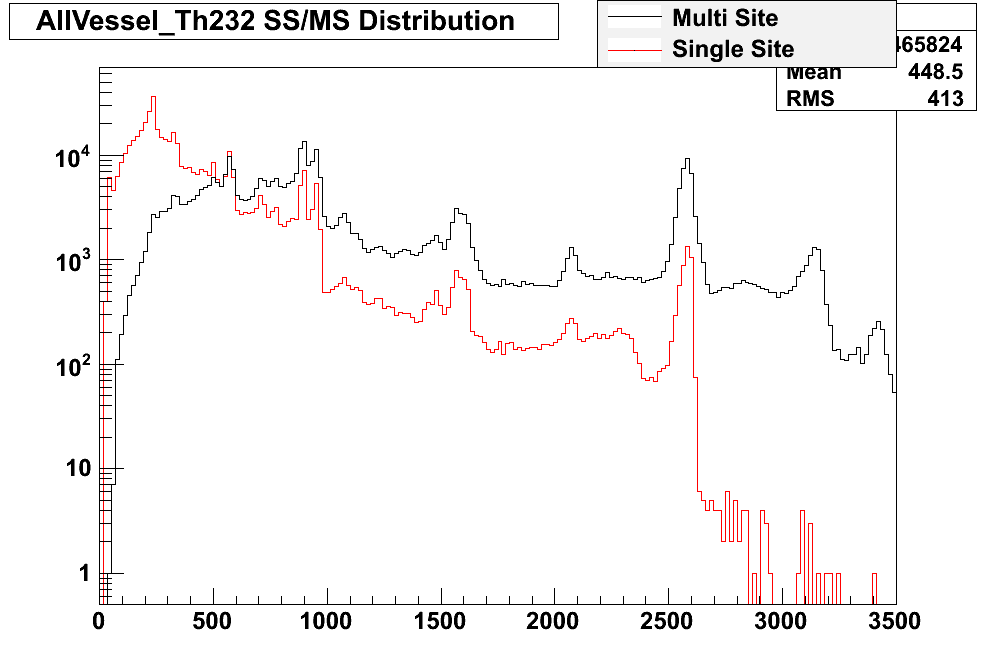
\includegraphics[keepaspectratio=true,width=\textwidth]{AllVessel_Th232_single_multi_site_spec.png}
\end{center}
\renewcommand{\baselinestretch}{1}
\small\normalsize
\begin{quote}
\caption{Energy spectra from $^{232}$Th in the TPC vessel; single-site and multi-site energy spectra are shown separately.~\cite{MCDocumentRun2a}}
\label{fig:ThGeantSpectra}
\end{quote}
\end{figure}
\renewcommand{\baselinestretch}{2}
\small\normalsize

The result of these GEANT simulations is a measurement of the efficiency with which events from various sources reach the liquid xenon, and also an understanding of the energy and position distributions of energy deposits from these sources.  Representative spectra of our primary backgrounds, $^{238}$U and $^{232}$Th, are shown in figures~\ref{fig:UGeantSpectra} and \ref{fig:ThGeantSpectra} respectively.

\subsection{Digitization of Waveforms}

After energy deposits are simulated using GEANT, it is necessary to model the conversion of those energy deposits into collection of scintillation and ionization, and then the generation of digitized waveforms resembling the waveforms which are collected in real data.

To generate a scintillation signal, a purely empirical model is used to estimate the relative signal magnitudes on the north and south APD planes.  This model only takes into account $Z$-dependence of the light collection, and does not incorporate the different light yields expected on each individual APD channel.  This model is therefore rather crude, and can only be used as a rough check on the signal-finding efficiency for scintillation as a function of energy.  Attempts to track optical photons in the TPC have met with only partial success which is insufficient to justify their significant computational cost.  Thus, the EXO simulations are unable to model most aspects of scintillation signals.  Section~\ref{sec:ResultFitting} will describe the methods used to cope with this aspect of simulation.

\begin{figure}
\begin{center}
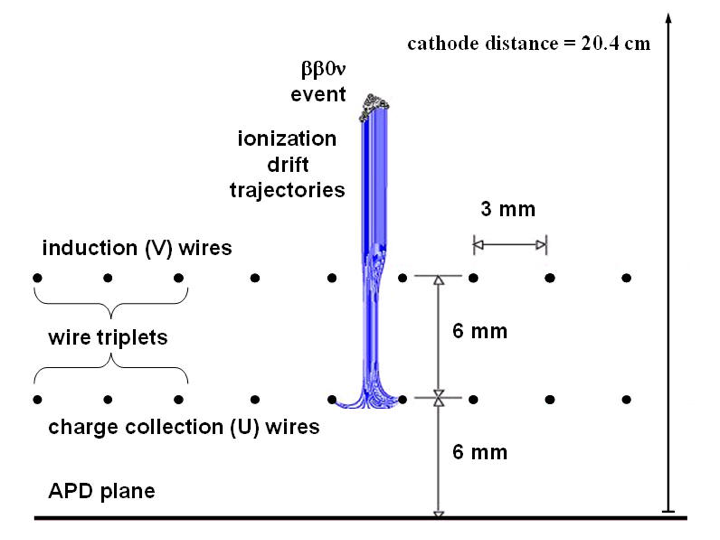
\includegraphics[keepaspectratio=true,width=\textwidth]{ChargeDrift2DModel.png}
\end{center}
\renewcommand{\baselinestretch}{1}
\small\normalsize
\begin{quote}
\caption{The wire planes are modeled in only two dimensions; charge drifts along the field lines, which are arranged to terminate only on the u-wires.~\cite{MCDocumentRun2a}}
\label{fig:TwoDimensionalWireModel}
\end{quote}
\end{figure}
\renewcommand{\baselinestretch}{2}
\small\normalsize

Simulation of charge signals is better-understood.  The detector is modeled by a two-dimensional geometry where, rather than one-dimensional wires arranged in two-dimensional planes, we have wire ``points'' at fixed voltage which are grouped in a one-dimensional pattern.  The v-wires are treated as stacked directly on top of the u-wires; it is impossible to model the true orientation of the v-wires which is rotated relative to the u-wires, but this has generally proven to be a negligible detail for us.  Only one TPC half is modeled because of the approximate mirror symmetry of the detector across the cathode.  Only a few wires are simulated in the second dimension because the electrostatic effect of any one wire will not extend beyond a few wire spacings.  This model is illustrated in figure~\ref{fig:TwoDimensionalWireModel}.~\cite{MCDocumentRun2a}

Electrostatic effects are simulated using the ANSYS Maxwell field simulator.  To simulate the electric fields in the detector, wires are treated as circles with a radius matching the approximate radii of the physical wires, with a constant voltage on their surfaces.  The APD plane and cathode plane are treated as constant-voltage boundaries, and a periodic boundary condition is established on the two remaining boundaries of the model geometry.

These electric fields can be used to trace the paths followed by charge deposits in the detector.  Charge deposits are drifted in small steps based on the direction of the electric field.  The speed of drift is taken from external measurements rather than from the magnitude of the electric field; in most of the bulk of xenon, the electric field and drift velocity are treated as constant, but near the u-wire plane the drift velocity is increased slightly to account for higher electric fields experienced in that region of the detector.  Charge attenuation due to finite purity can be modeled at this step, but generally is treated as infinite here; charge diffusion effects are ignored.

\begin{figure}
\begin{center}
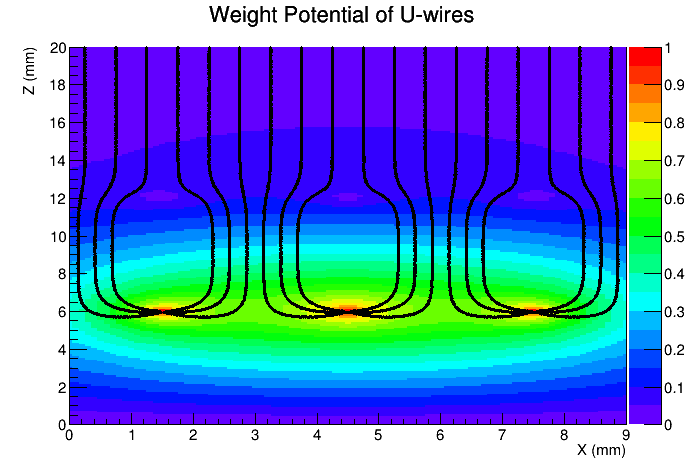
\includegraphics[keepaspectratio=true,width=\textwidth]{WeightPotContoursU_WithE.png}
\end{center}
\renewcommand{\baselinestretch}{1}
\small\normalsize
\begin{quote}
\caption{Weight potential of a u-wire channel consisting of three ganged wires.  Electric field lines are superimposed.~\cite{MCDocumentRun2a}}
\label{fig:UWireWeightPotential}
\end{quote}
\end{figure}
\renewcommand{\baselinestretch}{2}
\small\normalsize

\begin{figure}
\begin{center}
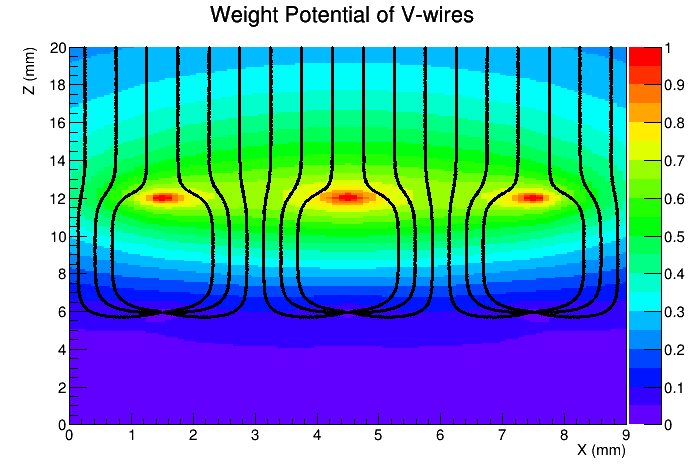
\includegraphics[keepaspectratio=true,width=\textwidth]{WeightPotContoursV_WithE.png}
\end{center}
\renewcommand{\baselinestretch}{1}
\small\normalsize
\begin{quote}
\caption{Weight potential of a v-wire channel consisting of three ganged wires.  Electric field lines are superimposed.~\cite{MCDocumentRun2a}}
\label{fig:VWireWeightPotential}
\end{quote}
\end{figure}
\renewcommand{\baselinestretch}{2}
\small\normalsize

We have discussed in section~\ref{sec:DetectorReadout} that charge is induced on the u-wires and v-wires; this means that we must record the amount of charge induced at each step along the drift path of the charge deposit.  This is done based on the Shockley-Ramo Theorem, which states that the change in induced charge $\delta q_i$ on an electrode $i$ is equal to:
\begin{equation}
\delta q_i = Q \delta W_i,
\end{equation}
where $Q$ is the total drifting charge and $W_i$ is the weighting potential of electrode $i$, defined as the potential which would be induced in our geometry if the potential on electrode $i$ were set to $1$ and the potential on all other boundaries were set to $0$.~\cite{ShockleyPaper}\cite{1686997}  Figures~\ref{fig:UWireWeightPotential} and~\ref{fig:VWireWeightPotential} illustrate the weighting potentials of a u-wire and v-wire channel, respectively.

Finally, the functions of integrated charge versus time must be converted to shaped digitized waveforms, and noise must be added.  The shaping and gain amplification is performed to match the electronics described in section~\ref{sec:DetectorReadout}.  To ensure accurate time shaping, the functions are all sampled at a bandwidth of $10$ MHz, and then downsampled after shaping to the nominal $1$ MHz.  Digitization is performed by converting voltages into units of ADC counts, then truncating to an integer value.  To model saturation effects, this number is pulled into the integer range $[0, 4096)$.

\begin{figure}
\begin{center}
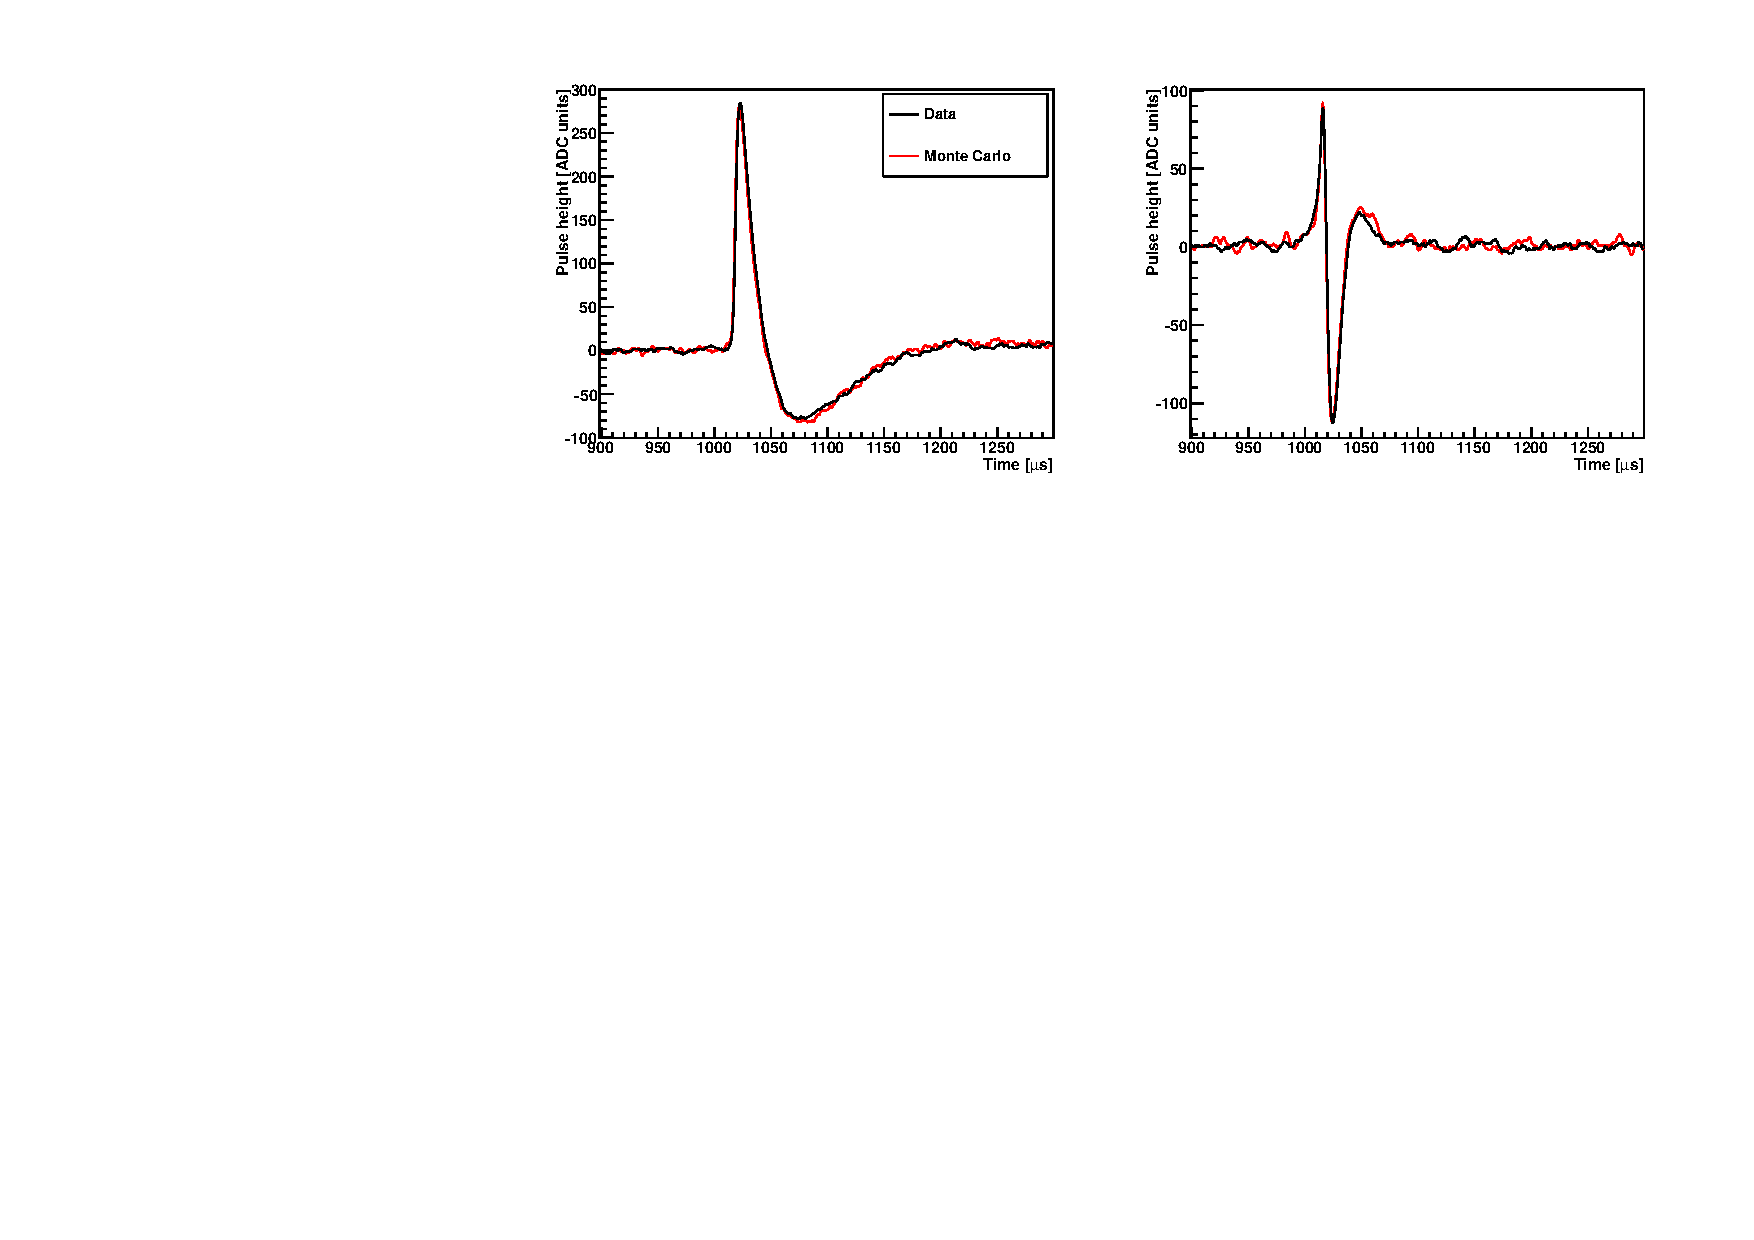
\includegraphics[keepaspectratio=true,width=\textwidth]{pulse_comp.pdf}
\end{center}
\renewcommand{\baselinestretch}{1}
\small\normalsize
\begin{quote}
\caption{Comparison between simulated and observed waveforms on a u-wire (left) and v-wire (right) from $^{228}$Th sources.  The events are chosen to have similar energies so that the magnitudes match.~\cite{MCDocumentRun2a}}
\label{fig:MCPulseComparison}
\end{quote}
\end{figure}
\renewcommand{\baselinestretch}{2}
\small\normalsize

Finally, we have found that the most effective way to add electronic noise to the signals is by extracting a set of representative noise waveforms from real data.  These are taken from a large number of solicited triggers which have been checked for the absence of a coincident event.  To increase the number of noise signals available, the noise waveforms sampled from the detector are spliced together, and simulated events may draw their noise from any subrange of the spliced-together noise waveform.  This method has been found to agree better with data than noise simulations using a random-number generator.  Figure~\ref{fig:MCPulseComparison} compares waveforms observed from a sample event in data and simulation.~\cite{MCDocumentRun2a}

\begin{figure}
\begin{center}
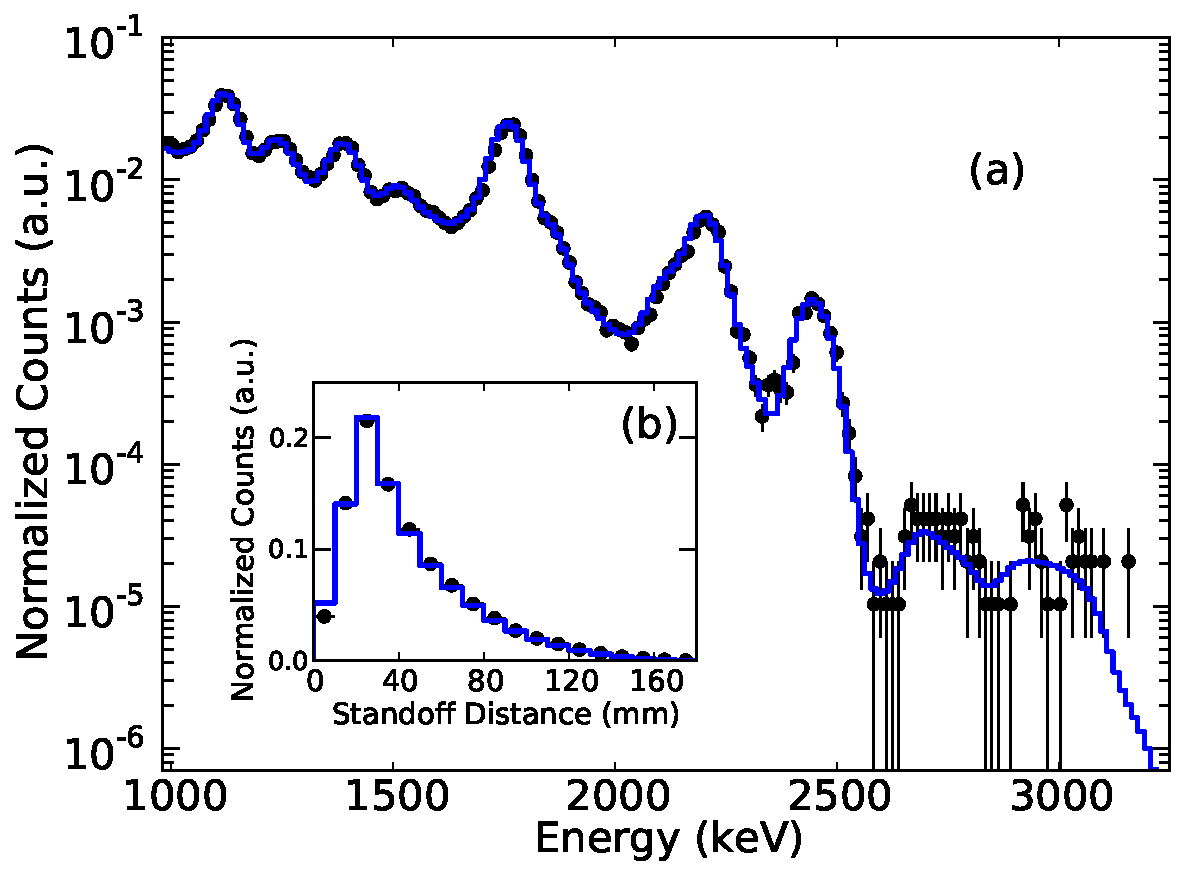
\includegraphics[keepaspectratio=true,width=\textwidth]{SS_Ra226_Campaign7.pdf}
\end{center}
\renewcommand{\baselinestretch}{1}
\small\normalsize
\begin{quote}
\caption{Comparison between simulated and observed energy spectra (a) and standoff distance (b) in single-site $^{226}$Ra events from a source located at position S5.~\cite{NewEXObb0nPaper_2014}}
\label{fig:RaSourceMCComparison}
\end{quote}
\end{figure}
\renewcommand{\baselinestretch}{2}
\small\normalsize

In this way, we are able to generate simulated data which in most respects resembles real data collected from the detector.  The EXO-200 simulation has shown remarkable agreement with the detector in the properties of energy and cluster location, as illustrated in figure~\ref{fig:RaSourceMCComparison}.  A significant effort has been made to achieve excellent agreement between simulation and data, and the result is that we can claim a strong understanding of the behavior of the EXO-200 detector.

\section{Cluster Reconstruction}\label{sec:ResultReconstruction}

The first stage of data processing involves locating candidate pulses in its waveforms, and fitting for the magnitude and time of any candidate pulses which are found.  The methods of accomplishing this will be described in sections~\ref{sec:ReconPulseFinding} and~\ref{sec:ReconPulseFitting}.  We will complete our description of cluster reconstruction with a brief explanation of the approach to the clustering of waveform pulses into three-dimensional clusters in section~\ref{sec:ReconClustering}.

\subsection{Pulse Finding}\label{sec:ReconPulseFinding}

Pulse-finding proceeds in two steps.  First, on all waveforms a matched filter is applied to do a preliminary search on all channels.  Then, a secondary search is performed on the u-wire signals to improve sensitivity to multiple signals near in time.

The matched filter algorithm was first described by D.O. North in 1943.~\cite{MatchedFilterPaper}  It attempts to decide between the null hypothesis that a waveform $X[\tau]$ consists of only noise and an alternative hypotheses that the waveform contains both signal and noise:
\begin{equation}\begin{cases}
H_0: & X[\tau] = n[\tau]\\
H_1: & X[\tau] = s[\tau] + n[\tau].
\end{cases}\end{equation}
We search for a linear functional $L_0$ which will act on $X[\tau]$ and maximize the expected signal-to-noise ratio,
\begin{equation}
SNR = \frac{\left(L_0\left\{s[\tau]\right\}\right)^2} {\left<\left(L_0\left\{n[\tau]\right\}\right)^2\right>}.
\end{equation}
In other words, if a waveform is composed of only noise, the functional should result in a small value; however, if the waveform contains signal then the functional should result in a large value.

The functional which maximizes the expected signal-to-noise ratio can be expressed as:
\begin{equation}
L_0\left\{X[\tau]\right\} = \mathcal{F}^{-1}\left\{ \frac{\mathcal{F}\left\{X\right\}[k] \mathcal{F}\left\{s\right\}^{*}[k]}{\left<\mathcal{F}\left\{N\right\}[k]\mathcal{F}\left\{N\right\}^{*}[k]\right>}\right\}[0],
\end{equation}
where $\mathcal{F}$ represents the Fourier transform.  This expression has an added benefit that if instead we'd like to test the hypothesis that the translated signal $s[\tau - \Delta]$ is contained in the waveform, we can do so with the test statistic:
\begin{equation}
L_\Delta\left\{X[\tau]\right\} = \mathcal{F}^{-1}\left\{ \frac{\mathcal{F}\left\{X\right\}[k] \mathcal{F}\left\{s\right\}^{*}[k]}{\left<\mathcal{F}\left\{N\right\}[k]\mathcal{F}\left\{N\right\}^{*}[k]\right>}\right\}[\Delta].
\end{equation}
Finally, we can define a test statistic $T$ for the waveform $X[\tau]$ to have a signal anywhere with:
\begin{equation}
T = \max_{\Delta} L_\Delta\left\{X[\tau]\right\}.
\end{equation}
This expression can be computed efficiently using the fast Fourier transform.  The time of the pulse is guessed as the value of $\Delta$ which led to the largest value of $L_\Delta\left\{X[\tau]\right\}$.

\begin{figure}
\begin{center}
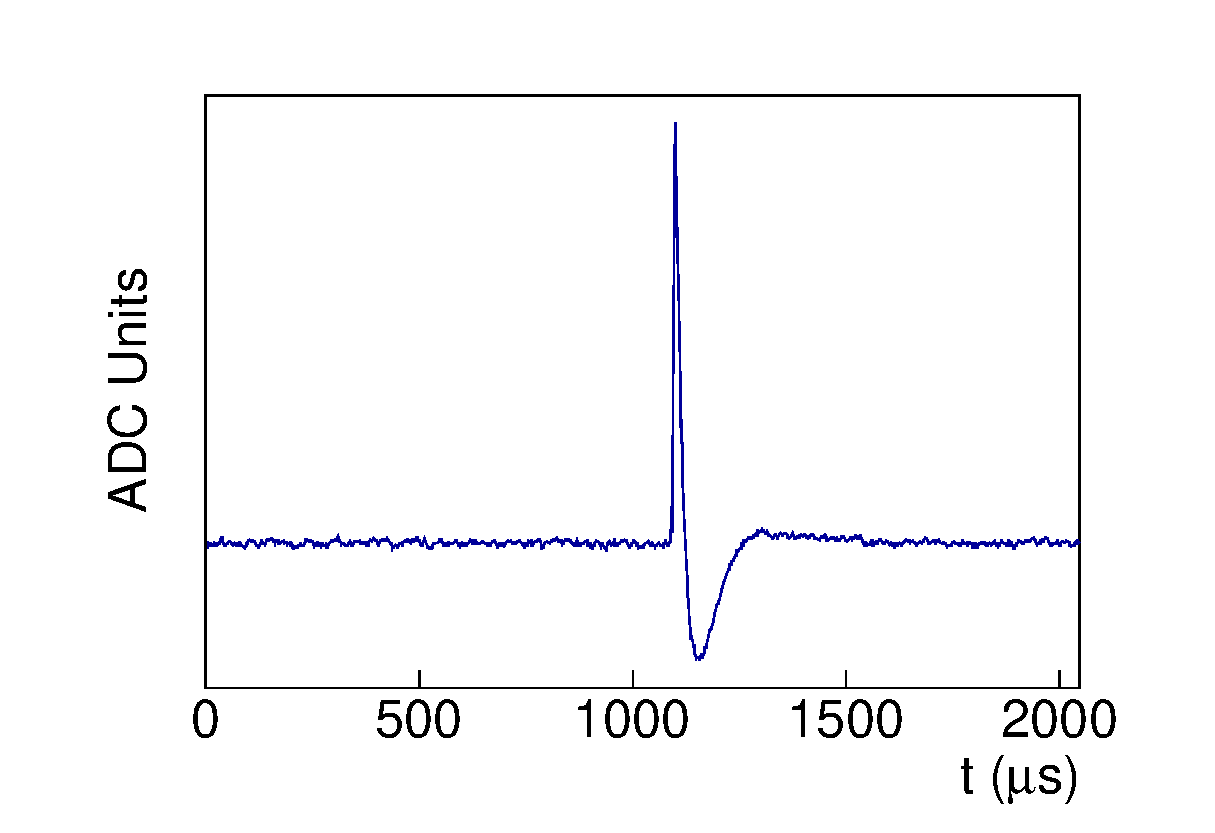
\includegraphics[keepaspectratio=true,width=.49\textwidth]{MFExamp_Raw.eps}
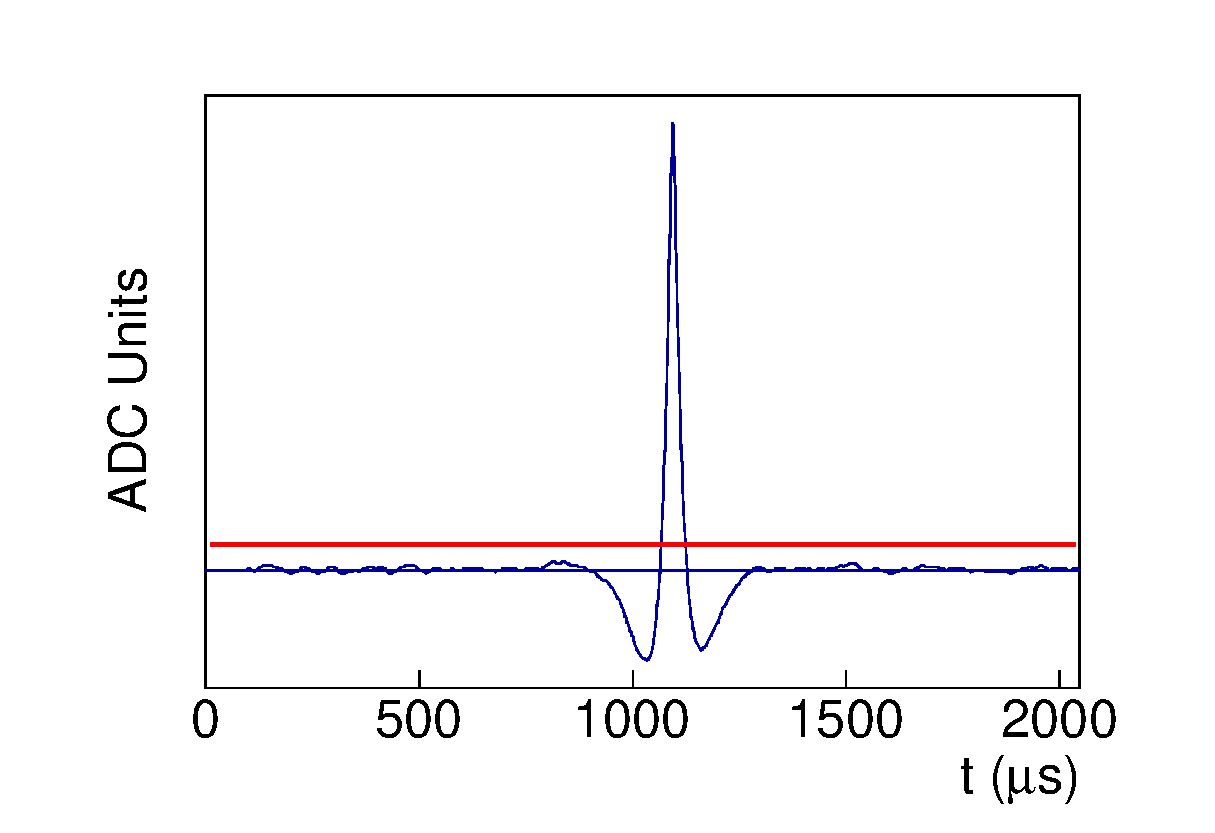
\includegraphics[keepaspectratio=true,width=.49\textwidth]{MFExamp_Applied.eps}
\end{center}
\renewcommand{\baselinestretch}{1}
\small\normalsize
\begin{quote}
\caption{A u-wire waveform (left) and the output from operation of the matched filter (right).  The red line on the right indicates our signal threshold; the matched filter output exceeds the threshold, so this waveform is determined to contain a signal.~\cite{ReconstructionDocument}}
\label{fig:MatchedFilterApplication}
\end{quote}
\end{figure}
\renewcommand{\baselinestretch}{2}
\small\normalsize

The first phase of pulse-finding performs a search using the matched filter on:
\begin{itemize}
\item All u-wire channels.
\item All v-wire channels.
\item The sum of all APD channels in the North plane.
\item The sum of all APD channels in the South plane.
\end{itemize}
An example application of the matched filter to a u-wire waveform is shown in figure~\ref{fig:MatchedFilterApplication}.

\begin{figure}
\begin{center}
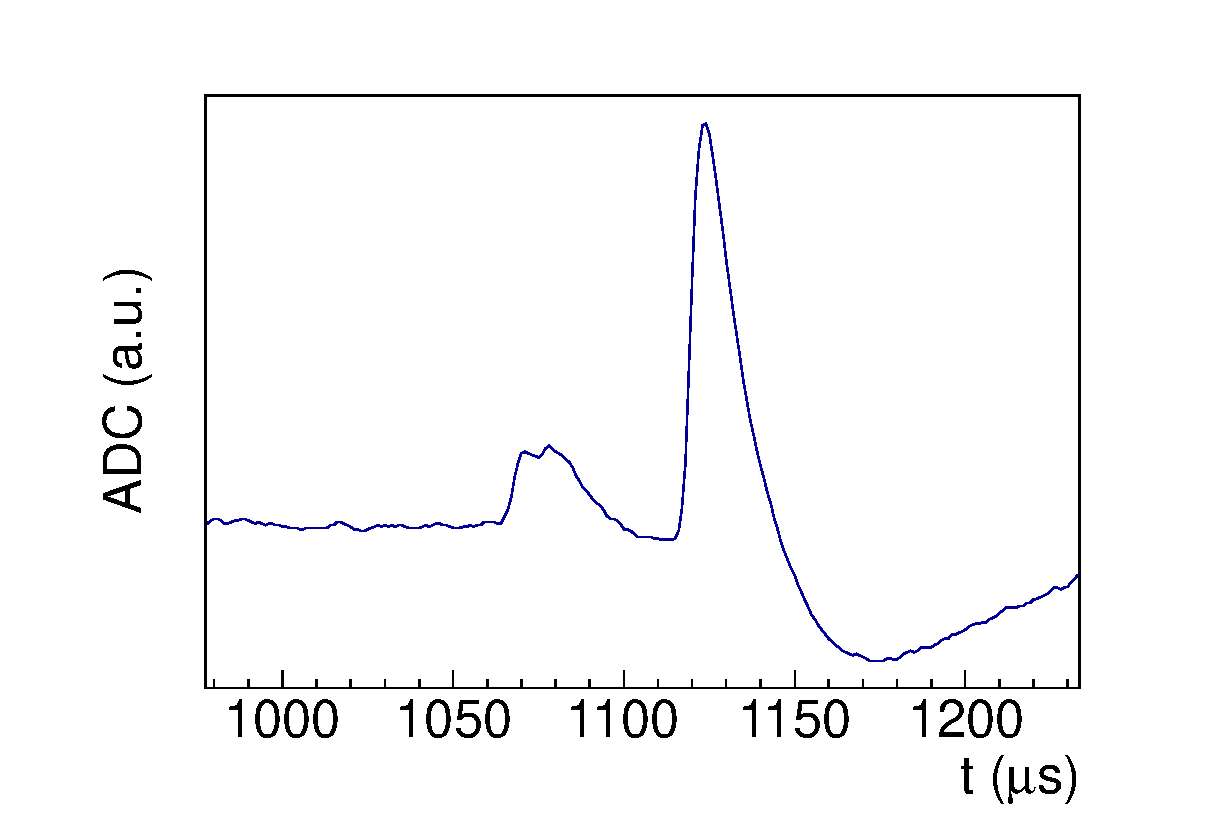
\includegraphics[keepaspectratio=true,width=.49\textwidth]{MSF_Raw.eps}
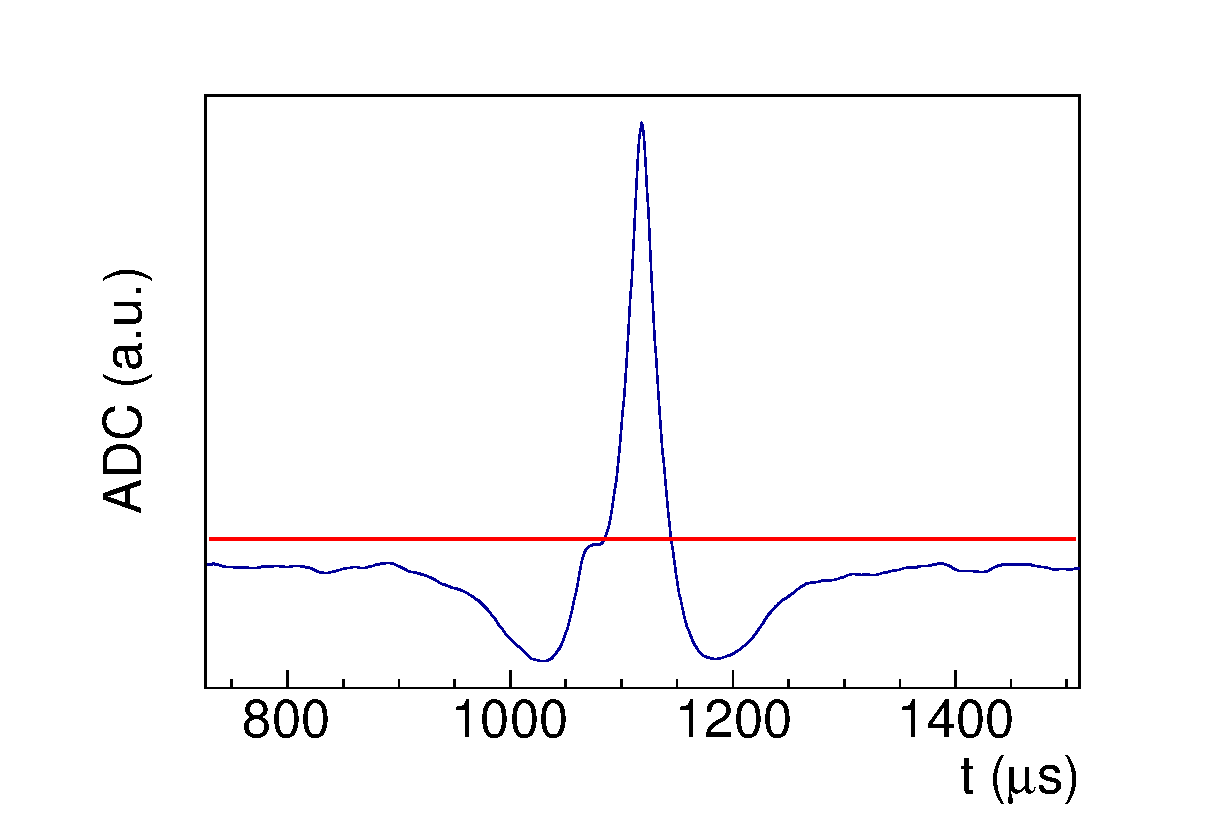
\includegraphics[keepaspectratio=true,width=.49\textwidth]{MSF_MatchedFilter.eps}
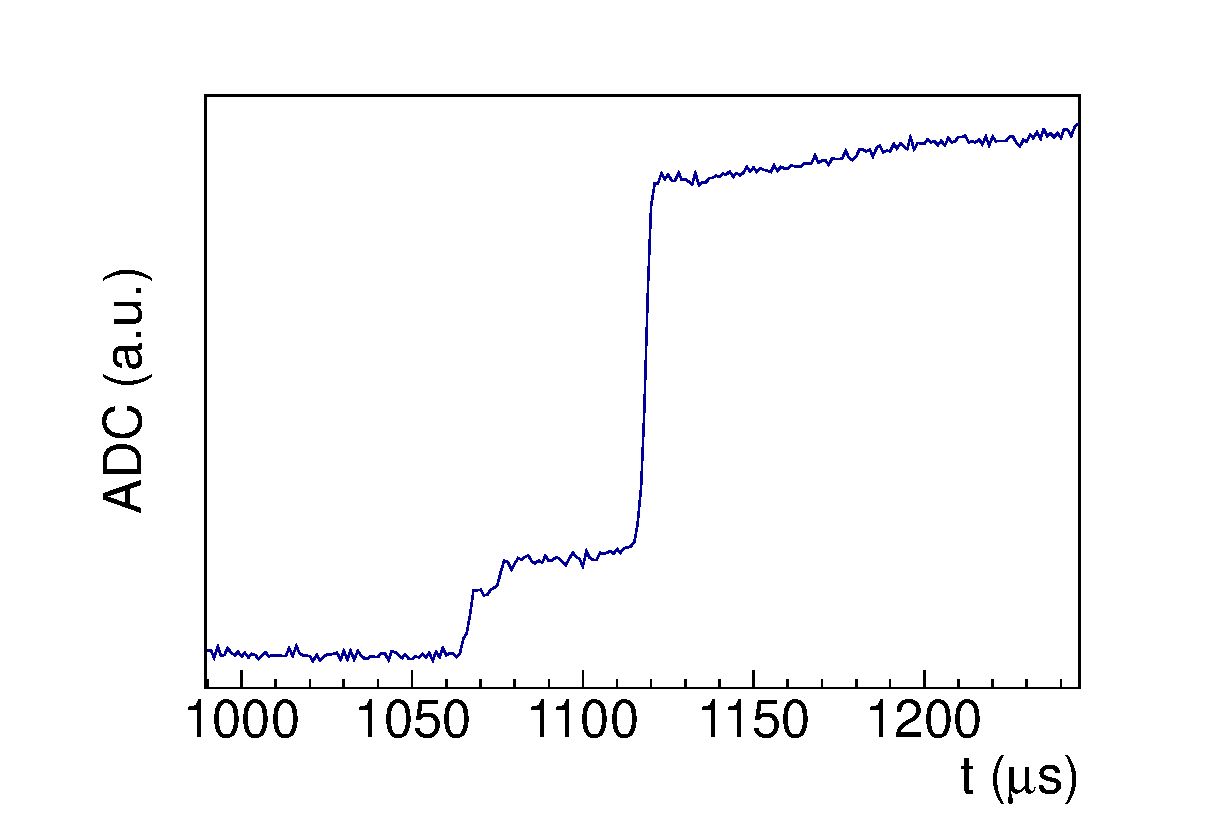
\includegraphics[keepaspectratio=true,width=.49\textwidth]{MSF_Unshaped.eps}
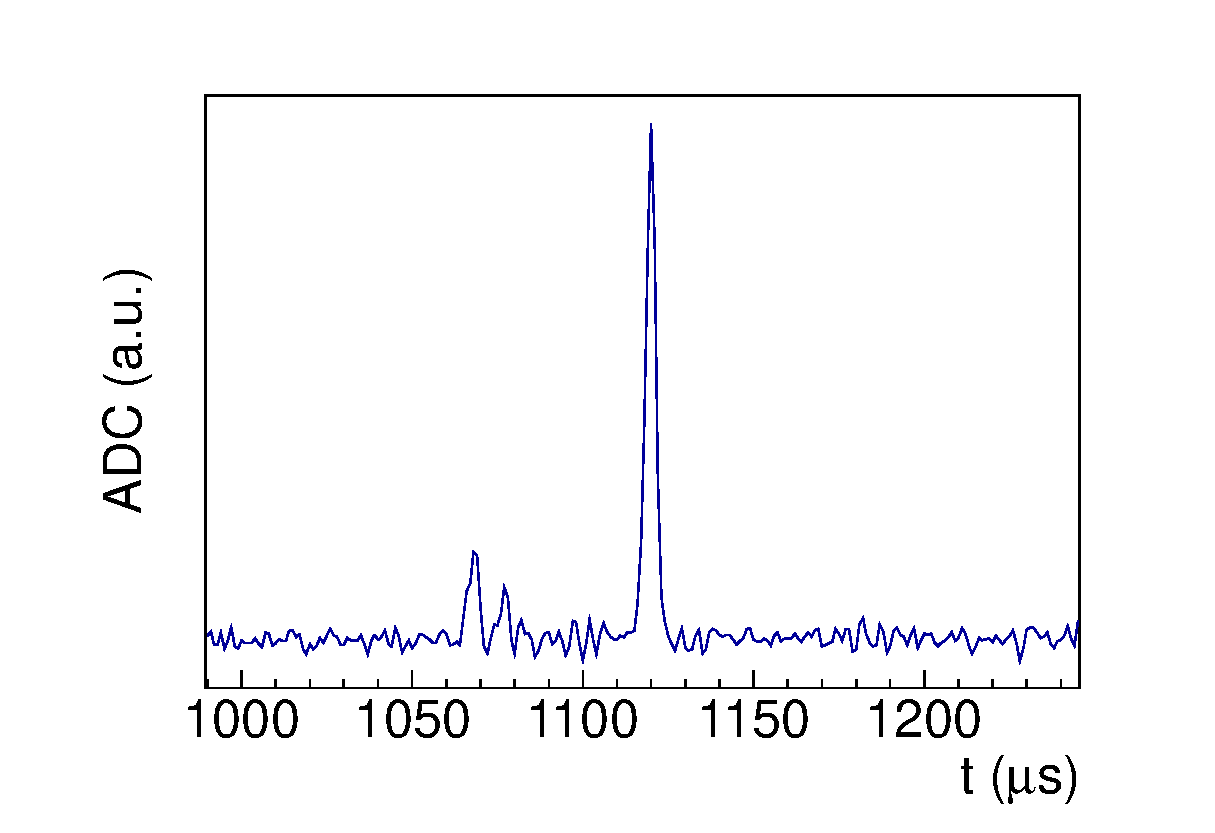
\includegraphics[keepaspectratio=true,width=.49\textwidth]{MSF_Reshaped.eps}
\end{center}
\renewcommand{\baselinestretch}{1}
\small\normalsize
\begin{quote}
\caption{A u-wire waveform composed of two signals near in time is shown (top left); the matched filter (top right) correctly detects the presence of signal, but does not detect the presence of two distinct signals.  At bottom left, the waveform is unshaped; at bottom right the waveform is reshaped with shorter differentiation times, leading to easier detection.~\cite{ReconstructionDocument}}
\label{fig:MultipleSignalFinderApplication}
\end{quote}
\end{figure}
\renewcommand{\baselinestretch}{2}
\small\normalsize

The matched filter has proven to be an excellent metric for deciding whether a waveform has a signal on it or not.  However, it is not as effective at distinguishing between the cases where one or multiple signals occur on a waveform.  We would particularly like to be able to classify u-wire waveforms by the number of distinct signals they contain because these generally provide the best sensitivity for single-site/multi-site discrimination.  The matched filter output function is designed to have a tall peak in the presence of a signal, but it may also be a broad peak which is difficult to resolve as the sum of two distinct signal contributions.

To improve sensitivity to multiple signals in u-wire waveforms, a second pass is performed on u-wire channels using a multiple-signal finder.  This scheme consists of first, unshaping the waveform offline to remove the effect of the shapers; and second, reshaping the waveform using shorter differentiation times than employed by hardware.  In a multiple-signal waveform, this has the effect of damping signals faster to reduce their overlap in time.  It is then possible to search for signals using a simple threshold which is not as sensitive to small signals as the matched filter, but is capable of detecting additional signals to complement the matched filter.  This process is illustrated in figure~\ref{fig:MultipleSignalFinderApplication}, and is the last procedure for finding signals.~\cite{ReconstructionDocument}

\subsection{Pulse Fitting}\label{sec:ReconPulseFitting}

After finding signals, it is necessary to perform a fit to the expected signal shape.  Fits are performed allowing both the signal magnitude and signal shape to float freely, where only the initial guesses for these parameters come from the finding step.  The metric for fits is a simple chi-square between waveform data and the expected signal shape, where error on each point is estimated by the root-mean-square noise of the channel.

\begin{figure}
\begin{center}
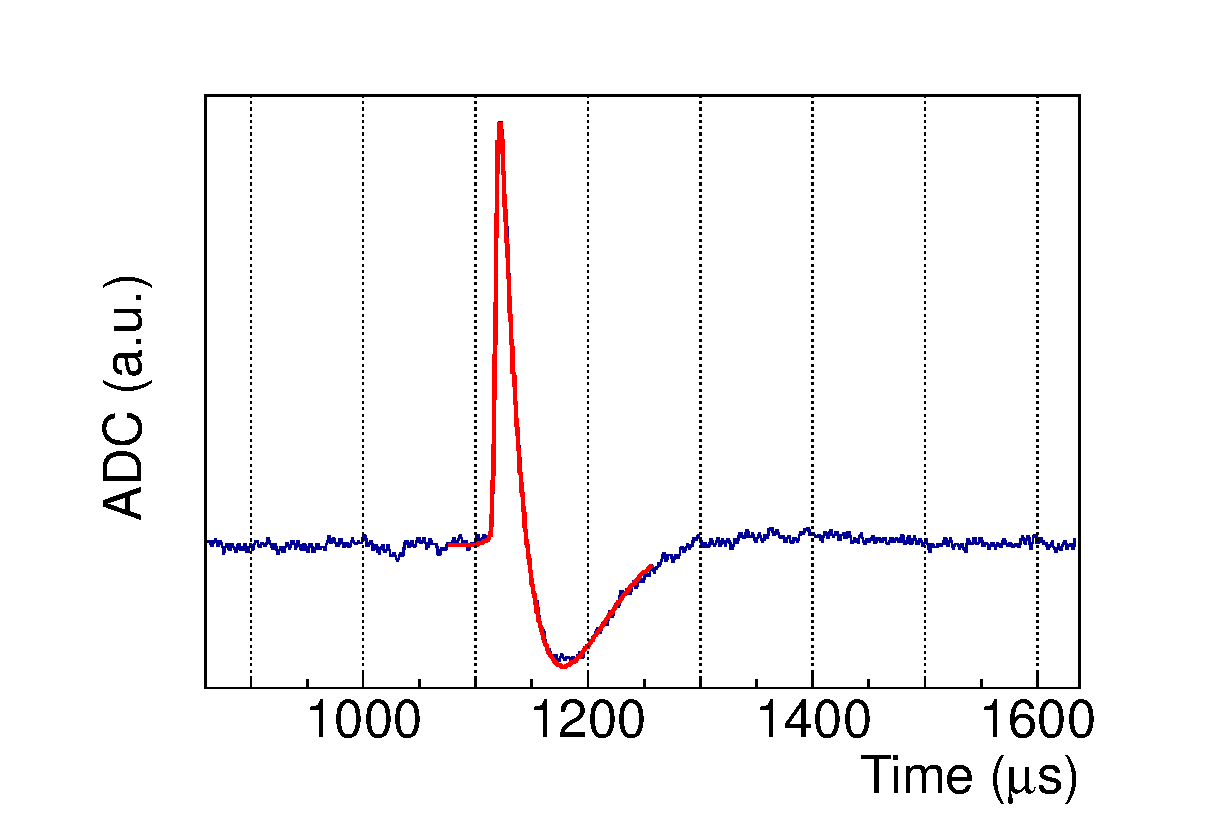
\includegraphics[keepaspectratio=true,width=.49\textwidth]{U_Wire_Fit.eps}
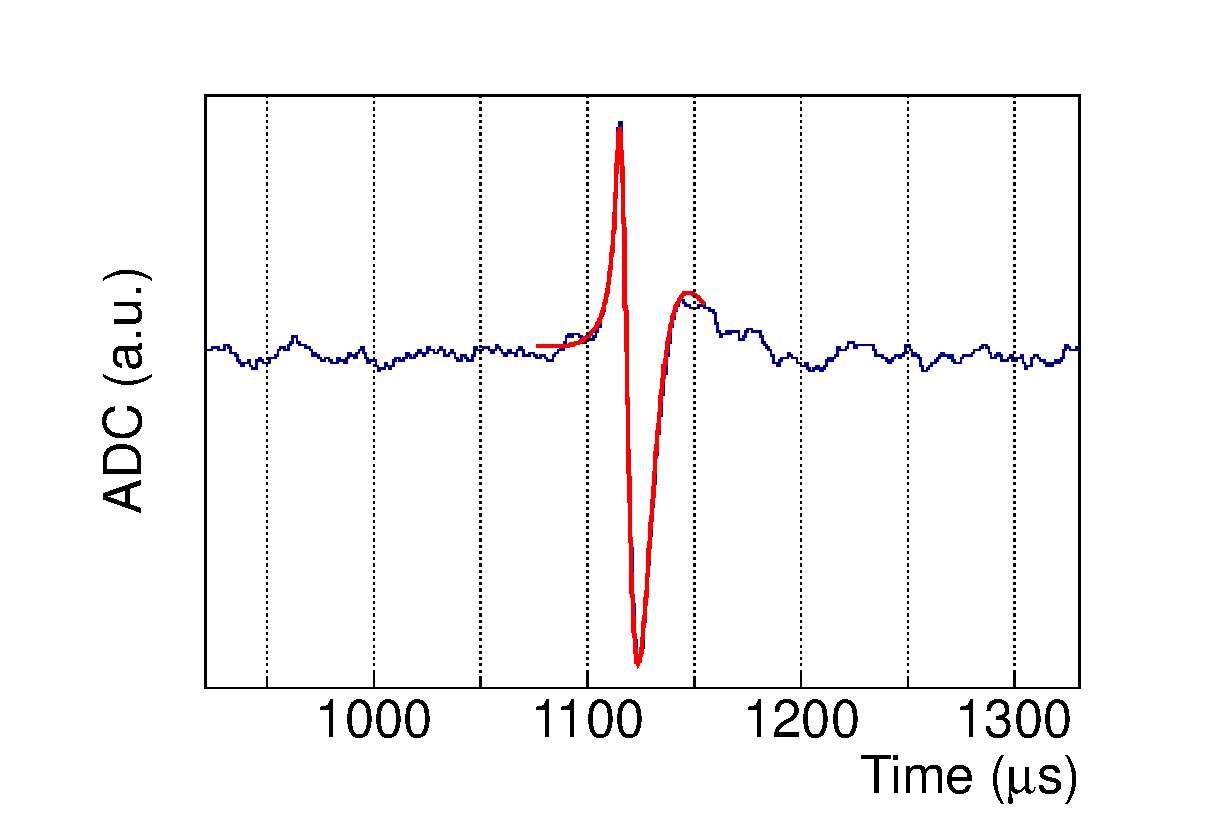
\includegraphics[keepaspectratio=true,width=.49\textwidth]{V_Wire_Fit.eps}
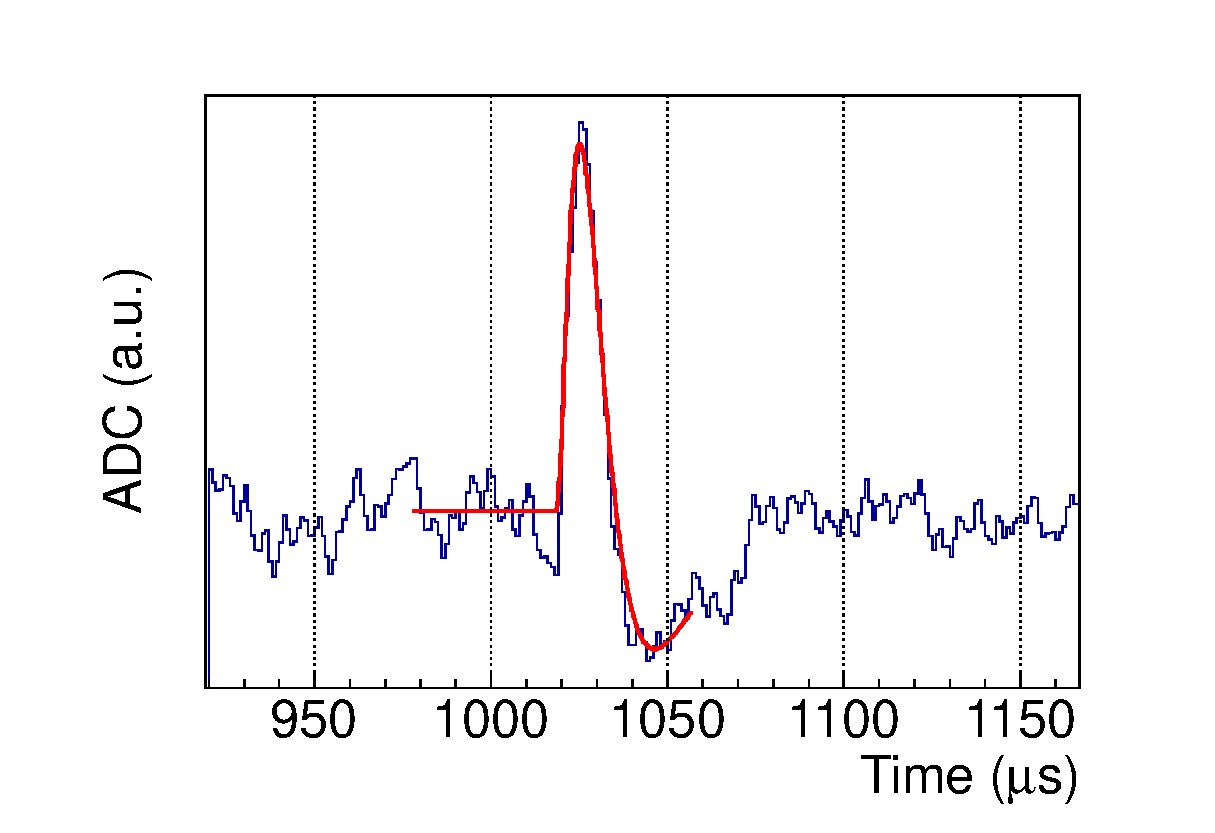
\includegraphics[keepaspectratio=true,width=.49\textwidth]{APD_Sum_Fit.eps}
\end{center}
\renewcommand{\baselinestretch}{1}
\small\normalsize
\begin{quote}
\caption{Fits to data for a u-wire (top left), v-wire (top right), and summed-APD waveform (bottom).  The red model line indicates the time extent of the fit window.~\cite{ReconstructionDocument}}
\label{fig:ReconExampleFits}
\end{quote}
\end{figure}
\renewcommand{\baselinestretch}{2}
\small\normalsize

To minimize the impact of signal templates which may be imperfect, and also to reduce the effect which waveform noise may have on our fit, we do not fit the entire waveform to our signal model.  Instead, we use only an $80 \mu$s fit window in the case of v-wires and APDs, and a $180 \mu$s fit window in the case of u-wires.  The fit windows are illustrated in example events in figure~\ref{fig:ReconExampleFits}.

As signal times and magnitudes are extracted, it may be discovered at this phase of processing that two signals which were reported by the finding phase are extremely close together in time.  In this case, we can generally conclude that the finding phase inadvertently reported the same signal multiple times; the multiple candidate signals should then be merged together, and the waveform refit.  The specific criteria for merging candidate signals includes a combination of signal timing and fit errors from a preliminary fit where all candidate signals are included; details can be found in~\cite{ReconstructionDocument}.

\subsection{Clustering Pulses into Deposit Sites}\label{sec:ReconClustering}


\section{Energy Corrections}\label{sec:ResultEnergy}

\subsection{Charge Corrections}\label{sec:ResultEnergyCharge}

\subsection{Light Corrections}\label{sec:ResultEnergyLight}

\section{Fitting}\label{sec:ResultFitting}

\section{Results and Physics Reach}\label{sec:ResultResults}

\section{Comparison to Results without Denoising}\label{sec:ResultComparison}

\section{Summary}\label{sec:ResultSummary}

\renewcommand{\thechapter}{8}
\chapter{Conclusions and Future Plans}
\label{ch:Conclusions}

This work has presented a wide-ranging upgrade to the scintillation waveform analysis of EXO-200.  The result has been a 21\% improvement in the single-site energy resolution at the $Q$-value, from 1.94\% to 1.53\% $\sigma/E$.  We strengthen the half-life limit of $\beta\beta 0\nu$ decay for this analysis by 11\%, corresponding to a 6\% stronger limit on the Majorana neutrino mass.  Separate background fits to the denoised and undenoised data indicate that the $2\sigma$ region of interest background is reduced 32\% by denoising, corresponding to a mean sensitivity which is strengthened by 17\% and a mean sensitivity for the Majorana mass which is 9\% lower than could be achieved without denoising.

\begin{figure}
\begin{center}
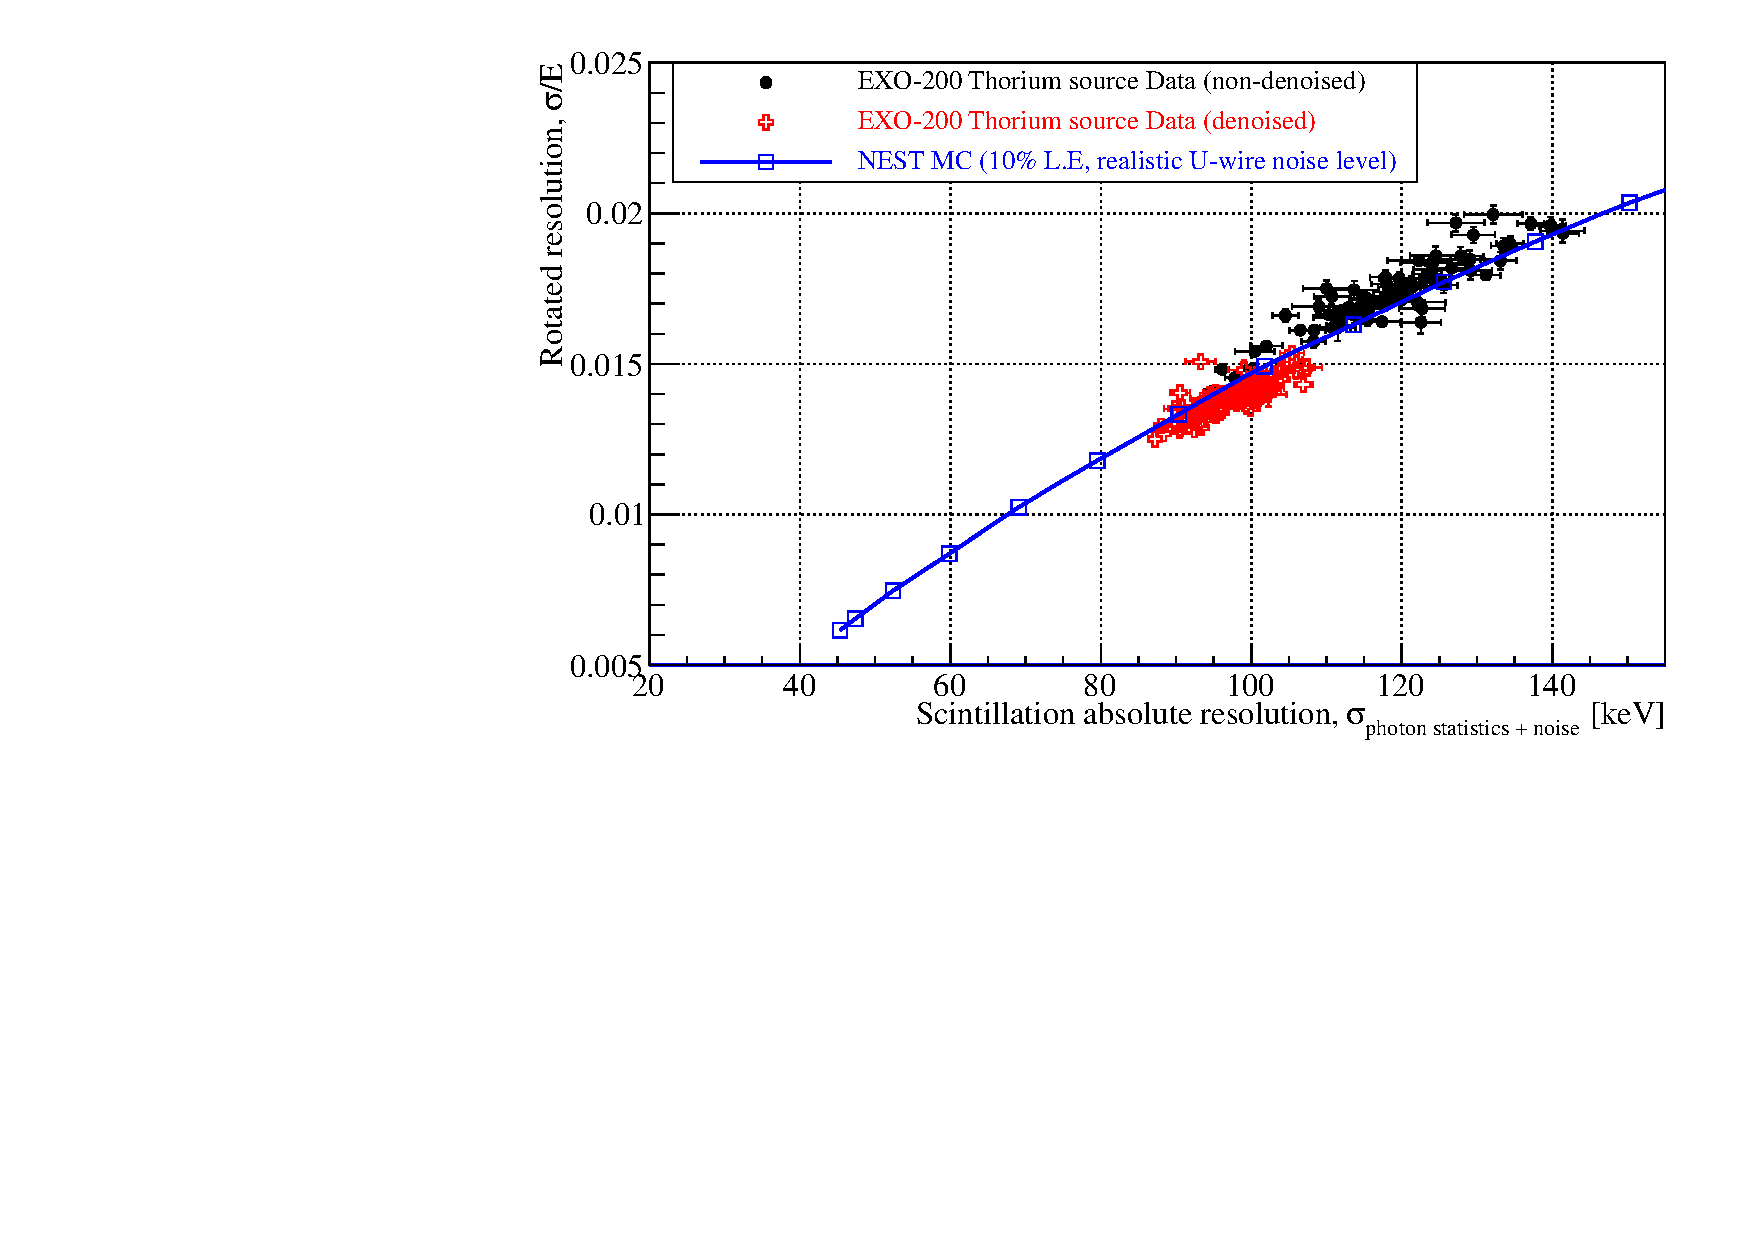
\includegraphics[keepaspectratio=true,width=\textwidth]{resoDataMC_800eRMSInIonization_Comp.pdf}
\end{center}
\renewcommand{\baselinestretch}{1}
\small\normalsize
\begin{quote}
\caption{NEST simulation software has been used to estimate how the rotated energy resolution at 2615 keV (vertical axis) depends on the scintillation-only resolution at 2615 keV (horizontal axis); this theoretical estimate is shown in blue, as applicable to the EXO-200 detector with fixed electric field.  Black points indicate measurements from thorium source runs without denoising; red points indicate measurements from thorium runs with denoising.  Figure provided by Liangjian Wen using NEST software~\cite{NESTpaper}.}
\label{fig:ScintillationVsOverallResolution_NEST}
\end{quote}
\end{figure}
\renewcommand{\baselinestretch}{2}
\small\normalsize

One question which must be asked is whether there is any room for further improvement in the energy resolution.  Figure~\ref{fig:ScintillationVsOverallResolution_NEST} shows simulations of the relationship between scintillation-only resolution and rotated energy resolution.  Points indicate the resolutions measured from denoised and non-denoised data; we can see that the model agrees well with both sets of data.  Based on these simulations, it is clear that further improvements to the scintillation resolution will indeed have a significant impact on the overall resolution of EXO-200; projections from figure~\ref{fig:BackgroundVsResolution} indicate that $^{232}$Th and $^{137}$Xe backgrounds can continue to be significantly reduced by resolution improvements, so these attempts are indeed worthwhile.

We have noted in section~\ref{sec:DenoisingInPractice} that the parameters used for this denoising are not optimal, and that preliminary studies indicate roughly 0.05 percentage points can be gained in overall energy resolution at 2615 keV with an up-to-date set of denoising parameters.  This issue is straightforward to address, and the next processing of our dataset will incorporate it.

Beyond this improvement, we have described in section~\ref{sec:ResultEnergyLight} that the denoised scintillation peak position displays a large position dependence which cannot be fully calibrated in downstream analysis.  The effect of this feature is to dilute our resolution improvements.  Although the cause of this position dependence is not fully understood, we believe that it originates in the lightmap because the lightmap is the input to denoising which encodes position-dependent yield information; one preliminary theory is that the discrepancy between 1-wire and 2-wire charge peak positions described in section~\ref{sec:ResultEnergyCharge} leads to a bias in event selection for the lightmap.  We believe that this issue can be addressed with further investigation and will lead to additional significant improvements in resolution.

The most exciting improvement in resolution may come not from offline analysis but from planned electronics upgrades.  There are indications that the source of electronic noise in the APDs is now understood and can be fixed in hardware in the near future, with an expectation of energy resolutions below 1\% after all upgrades~\cite{ElectronicsUpgradeReport_March2014}.  Energy resolution improvements on this scale would have a significant impact on backgrounds and the sensitivity of EXO-200 to $\beta\beta 0\nu$ decay.

One may wonder, after a hardware upgrade which reduces electronic noise on the APDs, whether denoising will still be a necessary component of the analysis.  It may indeed be the case that the full denoising scheme is not needed for lower-noise waveforms.  However, certain components of this analysis will still be critical to good resolution.  In particular, the techniques developed in this work to measure an APD-by-APD lightmap will still be needed to relate pulse magnitudes to deposit energies; we have seen hints in section~\ref{sec:ResultComparisonEnergy} that application of channel-dependent gain corrections reduces their impact on energy resolution by a factor of 9.7 in single-site data, and if true then this will be a critical component of any scintillation measurements regardless of changes in electronic noise.

Beyond energy resolution upgrades to EXO-200, the techniques described in this work have led to the most complete understanding to date of what limits the energy resolution of EXO-200.  This understanding is timely because the successor experiment to EXO-200, called nEXO, is currently in design stages of development.  Options for nEXO which are currently being considered include the types of light sensors to use and how much to gang sensors together; studies are currently underway to understand exactly how design decisions have impacted EXO-200 scintillation energy resolution, and the results will provide useful feedback to the nEXO design process.

Additionally, other aspects of the EXO-200 analysis besides energy resolution may benefit from the progress discussed here.  It may be possible that our improved understanding of scintillation enables us to enlarge the EXO-200 dataset.  Currently, data taken between May 2011 and October 2011 is not used in the $\beta\beta 0\nu$ search because it was prior to a u-wire electronics upgrade and an increase in the APD bias voltages.  Studies which used that data were primarily charge-driven and only used scintillation to measure Z-positions of deposits.  However, it is possible that denoising will permit us to make use of the weaker scintillation pulses from that dataset and achieve an acceptable energy resolution; the result could be months of added livetime for future studies.

Our deeper understanding of the scintillation pulses from an individual-APD lightmap also has the potential to improve our pulse-finding threshold.  The EXO-200 energy threshold of 980 keV is limited by scintillation-finding.  A lower energy threshold would not directly impact a $\beta\beta 0\nu$ search, but would allow backgrounds to be better-constrained by fits.  Furthermore, there are low-energy physics searches like $^{134}$Xe $\beta\beta 2\nu$ decay and $^{136}$Xe $\beta\beta 0\nu \chi$ Majoron decay searches which have not been described in this work but which would benefit strongly from a lower energy threshold~\cite{ThesisSteve}.  Currently all scintillation pulses are found on summed APD waveforms; our detailed APD lightmap should permit us to make use of individual-APD information, which may permit better noise rejection and lead to a lower pulse-finding threshold.

Another set of alternative physics searches which could be improved using techniques from this work are excited-state decay searches.  We expect $^{136}$Xe to have a $\beta\beta 2\nu$ decay mode to the second excited state of $^{136}$Ba, followed by the prompt emission of two de-excitation gammas.  Currently the EXO-200 analysis only produces scintillation measurements for all simultaneous charge deposits together, making it impossible to generate anticorrelated energy estimates for single energy deposits.  However, a natural extension of denoising would permit us to extract separately the scintillation energies of each deposit site, using knowledge of which channels collected photons to assign energy appropriately.  By enabling anticorrelated individual-site energy measurements, we could improve our ability to identify the clusters produced by each of the de-excitation gammas from an excited-state decay.

Finally, there is a possibility, remote but tantalizing, that a variation of these methods could lead to improved discriminating power between beta and gamma deposits.  The leading edge of u-wire pulses includes information about the size of the charge cloud: a diffuse charge cloud penetrates the v-wire shielding grid slowly, leading to a slowly-rising leading edge to the u-wire pulse, whereas a more pointlike charge cloud penetrates the v-wire shielding grid in a shorter span of time and leads to a sharply-rising leading edge to the u-wire pulse, so the risetime of a pulse may provide information about the size of its charge cloud.  The leading edge of the u-wire pulse is quite short, contained in only a few samples, and current studies have shown no significant improvement in discriminating power when it is used; however, simulations hint that it should be possible to use this information.  One plan for improving the quality of this discriminator is to denoise the u-wire waveforms so that the samples from the leading edge of the pulse are less noisy and provide a better measure of the risetime of the pulse.  Improved ability to discriminate betas from gammas would lead to fewer backgrounds for $\beta\beta 0\nu$ decay, improving our sensitivity further.

These are some of the many ways in which the denoising techniques of this work may be applied.  In all of these applications, the broader message we take away from denoising is that having a complete model of a detector's signals is a powerful thing.  We have constructed a full description of the APD noise correlation behavior and a complete characterization of how photons generate pulses on waveforms and with what fluctuations.  Neither tool was available previously, and using them we have been able to transform the challenge of improving energy resolution into a purely mathematical optimization.    We have confidence that these same tools will yield benefits in many EXO-200 analyses to come.




\renewcommand{\baselinestretch}{1}
\small\normalsize
\newpage
\phantomsection % Needed to make hyperlinks point to the right page.
\addcontentsline{toc}{chapter}{Bibliography}
\bibliographystyle{thesisbibstyle}
\bibliography{Bibliography}

\end{document}
